\documentclass[xcolor=dvipsnames,table]{beamer}
%%%%%%%%%%%%%%%%%%%%%%%%%%%%%
\usepackage{talk}
\usepackage{soul}
%%%%%%%%%%%%%%%%%%%%%%%%%%%
\usepackage{array}   % for \newcolumntype macro
\newcolumntype{L}{>{$}l<{$}} % math-mode version of "l" column type
\newcolumntype{R}{>{$}r<{$}} % math-mode version of "r" column type
\newcolumntype{C}{>{$}c<{$}} % math-mode version of "c" column type
\usepackage{booktabs}
%%%%%%%%%%%%%%%%%%%%%%
%\usepackage{mycolors}
\usepackage{fp}
\usepackage{multirow}
%\usepackage{coloremoji}
\newcommand{\arXiv}[1]{\href{https://arxiv.org/abs/#1}{arXiv:#1}}
\widescreen

\newenvironment<>{varblock}[2][.9\textwidth]{%
  \setlength{\textwidth}{#1}
  \begin{actionenv}#3%
    \def\insertblocktitle{#2}%
    \par%
    \usebeamertemplate{block begin}}
  {\par%
    \usebeamertemplate{block end}%
  \end{actionenv}}


% set block transparency: https://tex.stackexchange.com/a/44716/59580
\addtobeamertemplate{block begin}{\pgfsetfillopacity{0.8}}{\pgfsetfillopacity{1}}
\addtobeamertemplate{block alerted begin}{\pgfsetfillopacity{0.8}}{\pgfsetfillopacity{1}}
\addtobeamertemplate{block example begin}{\pgfsetfillopacity{0.8}}{\pgfsetfillopacity{1}}


\title{ Scotogenic seesaw and baryogenesis }
\subtitle{with gauged Baryon number}


%\subtitle
%{Reconstruction of the neutrino mass matrix} % (optional)

\author{Diego Restrepo
}
% - Use the \inst{?} command only if the authors have different
%   affiliation.
\institute{
  \begin{picture}(100,2)
    \put(230,-110){ %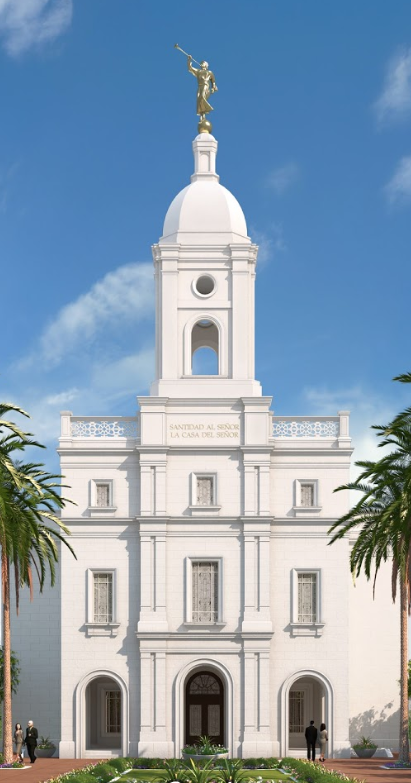
\includegraphics[scale=0.17]{temple}
    }
\end{picture}
  \affiliation{\tiny Instituto de Física\\
Universidad de Antioquia\\
Phenomenology Group %\\
%\& UNICAMP
}%
{http://gfif.udea.edu.co}%
{}%
{ufsm}% small image here, use pixel for nothing
{}
\arxiv{ arXiv:2205.05762
%  arXiv:1812.05523 [PRD], 1906.09685 [PRD], 1907.11938, 1909.09574
}
\collaborators{ Andrés Rivera (UdeA), Walter Tangarife (Loyola University Chicago)
%  Carlos Yaguna (UPTC), Julian Calle, Óscar Zapata, David Suárez
}
}

\date{\tiny %December 3, 2019 - COMHEP

  %[PDF: \url{http://bit.ly/comhep2019}]
} % (optional) \today
%{
\includegraphics[scale=0.3]{udea}}
\titlegraphic{\hfill
\includegraphics[height=1.5cm]{udea}}

%\subject{Talks}
% This is only inserted into the PDF information catalog. Can be left
% out. 


% If you have a file called "university-logo-filename.xxx", where xxx
% is a graphic format that can be processed by latex or pdflatex,
% resp., then you can add a logo as follows:

% \pgfdeclareimage[height=0.5cm]{university-logo}{university-logo-filename}
% \logo{\pgfuseimage{university-logo}}



% Delete this, if you do not want the table of contents to pop up at
% the beginning of each subsection:
%\AtBeginSubsection[]
%{
%  \begin{frame}<beamer>
%    \frametitle{Outline}
%    \tableofcontents[currentsection,currentsubsection]
%  \end{frame}
%}
\setbeamercolor{block title}{bg=black!90,fg=white}

\newcommand{\chml}[2]{$\underline{\text{#1\hspace{#2}}}$}
\begin{document}


%=============== 
\begin{comentar}
%===============  
%=============
\end{comentar}
%=============

\maketitle

\section{Model building}

\begin{frame}
  \frametitle{Lie groups}


  \begin{center} 
  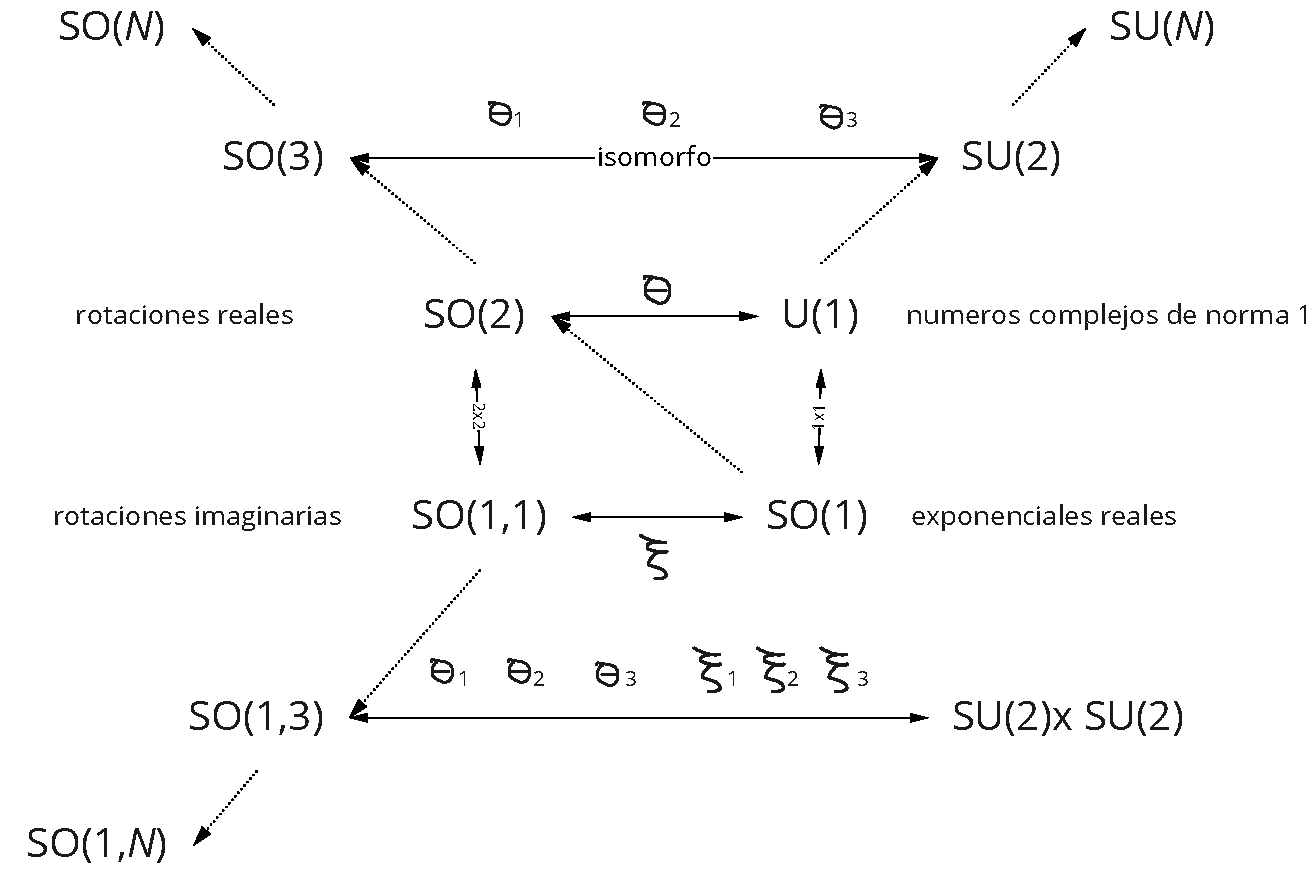
\includegraphics[scale=0.4]{sunson}
  \end{center}  

\vspace{-1cm}


\begin{align}
  U=\exp \left( i \sum_j T_j \theta^{j} \right),
\end{align}
where $\theta^j$ are the parameters of the transformation and  $T_j$ are the generators.
\end{frame}



\subsection{$\operatorname{SO}(1)$}
\begin{frame}[fragile,allowframebreaks]
Consider the $1\times1$
\begin{align}
  K=-i\,,
\end{align}
which generates an element of dilaton group , $\operatorname{SO}(1)$, $R(\xi)$
\begin{align}
  \lambda(\xi)=\operatorname{e^{\xi}}\,,
\end{align}
which are just the group of the real exponentials. Such a number can be transformed as
\begin{align}
  x\to x'=\operatorname{e^{\xi}}x\,,
\end{align}
that corresponds to a boost by $\operatorname{e^{\xi}}$.
We can defin the invariant scalar product just as the division of real numbers, such that
\begin{align}
  x\cdot y \to x'\cdot y'\equiv \frac{x'}{y'}= \frac{\operatorname{e}^{\xi}x}{\operatorname{e}^{\xi}y}=\frac{x}{y}=x\cdot y\,.
\end{align}
\end{frame}



\begin{frame}[fragile,allowframebreaks]

Under a general Lorentz transformation we have.
\begin{equation}
  \label{eq:xx5}
  A^\mu(x)\to A^{\prime \mu}(x)={\Lambda^\mu}_{\nu}A^\nu(\Lambda^{-1}x).
\end{equation}

A pure underscript 4-vector is
\begin{align}
   \partial_\mu=\frac{\partial}{\partial x^\mu}=&\left(
    \frac{\partial}{\partial t},\frac{\partial}{\partial x},\frac{\partial}{\partial y},\frac{\partial}{\partial z}
  \right)
  =(\partial_0,\boldsymbol{\nabla}).
\end{align}

From
\begin{align}
  \label{eq:183qft}
    \frac{1}{{x'}^\mu}= {\left(\Lambda^{-1}\right)^\nu}_\mu\frac{1}{x^\nu}\,,
\end{align}
the tranformation properties for a $\partial_\mu=\partial/\partial x^\mu$, are
\begin{align}
  \label{eq:dmulrtran}
   {\partial\,}'_\mu=& {\left(\Lambda^{-1}\right)^\nu}_\mu\partial_\nu\,.
\end{align}

In this way, the invariant scalar product between the 4-vector field and the four-gradient is just
\begin{align}
  \partial_\mu A^\mu\to   \partial'_\mu A^{\prime \mu}= \partial_\mu A^\mu\,.
\end{align}


\end{frame}


\begin{frame}[fragile,allowframebreaks]

\begin{table}
  \centering
   \begin{tabular}{lll}
    Name & Symbol & $\operatorname{SU(N)}$ \\\hline
    scalar $N$-plet  & $\Psi$ & $U \Psi$ \\
    scalar anti-$N$-plet  & $\Psi^\dagger $ & $\Psi^\dagger U^\dagger $ \\\hline
    \end{tabular}\hspace{3cm}
   \begin{tabular}{lll}
    Name & Symbol & Lorentz \\\hline
    Photon & $A^\mu$ & ${\Lambda^\mu}_\nu A^\nu$ \\
    4-gradient & $\partial_\mu$ & $\partial_\nu {\left(\Lambda^{-1}\right)^\nu}_\mu$ \\\hline
  \end{tabular}
  \caption{
       Scalar products: $\Psi^\dagger \Psi$,  \hspace{4cm}
       $\partial_\mu A^{\mu}\,,\quad A^\nu A_\nu \,,\quad \partial_\mu  \partial^\mu$
}
  \label{tab:fermionlr}
\end{table}


\begin{table}
  \centering
  \begin{tabular}{llll}
    Name & Symbol & Lorentz & $U(1)$\\\hline
    $e_L$: electron {\color{red}left} & $\xi_{\color{red}\alpha}$ & ${S_{\color{red}\alpha}}^{\color{red}\beta}\xi_{\color{red}\beta}$ & $e^{i\theta}\xi_{\color{red}\alpha}$\\
   $\left( e_L \right)^{\dagger}$: positron {\color{blue}right}   & $\left( \xi_{\color{red}\alpha} \right)^{\dagger}=\xi^{\dagger}_{\color{blue}\dot{\alpha}}$ & $\xi^{\dagger}_{\color{blue}\dot{\beta}}{\left[{S^{\dagger}}\right]^{\color{blue}\dot{\beta}}}_{\color{blue}\dot{\alpha}}$ & $\xi^{\dagger}_{\color{blue}\dot{\alpha}}e^{-i\theta}$\\
   $e_R$: electron {\color{blue}right}   & $\left( \eta^{\color{red}\alpha} \right)^{\dagger}=\eta^{\dagger\;\color{blue}\dot{\alpha}}$ & ${\left[ \left( S^{-1} \right)^\dagger \right]^{\color{blue}\dot{\alpha}}}_{\color{blue}\dot{\beta}}\eta^{\dagger\;\color{blue}\dot{\beta}}$& $e^{i\theta}\eta^{\dagger\;\color{blue}\dot{\alpha}}$\\
   $\left( e_R \right)^{\dagger}$: positron {\color{red}left}&$\eta^{\color{red}\alpha}$& $\eta^{\color{red}\beta}{\left[ S^{-1}  \right]_{\color{red}\beta}}^{\color{red}\alpha}$ & $e^{-i\theta}\eta^{\color{red}\alpha}$\\\hline
  \end{tabular}
  \caption{electron components}
  \label{tab:electron}
\end{table}



Scalar products
\begin{itemize}
\item Majorana scalars: $\xi^{\alpha}\xi_{\alpha}+\xi^{\dagger}_{ \dot{\alpha}}\xi^{\dagger \dot{\alpha}}$, $\eta^{\alpha}\eta_{\alpha}+\eta^{\dagger}_{ \dot{\alpha}}\eta^{\dagger \dot{\alpha}}$.
\item Dirac scalar: $\eta^{\alpha}\xi_{\alpha}+ \xi^{\dagger}_{\dot{\alpha}}\eta^{\dagger\;\dot{\alpha  }} $.


 \item Scalar under subgroup $\operatorname{SL}(2,C)$ but vector under $\operatorname{SO}(1,3)$: $ S^\dagger\overline{\sigma}^\mu S={\Lambda^\mu}_\nu\overline{\sigma}^\nu$
\end{itemize}


\end{frame}

\begin{frame}[fragile,allowframebreaks]
\begin{table}
  \centering
    \begin{tabular}{|l|c|c|c|l|}\hline
      Field               &Lorentz   & SU(3)$_{C}$            & SU(2)$_{L}$           & U(1)$_Y$          \\\hline
    $Q   $                 & $\xi_{\alpha}^1$ & $\mathbf{3}$           & $\mathbf{2}$          & $1/6$          \\      
    $L   $                 & $\xi_{\alpha}^2$ & $\mathbf{1}$           & $\mathbf{2}$          & $-1/2$          \\
    $\left(u_R^{-}\right)^{\dagger}$ & $\eta_1^\alpha$  & $\overline{\mathbf{3}}$ & $\mathbf{1}$           & $-2/3$              \\
    $\left(d_R^{-}\right)^{\dagger}$ & $\eta_2^\alpha$  & $\overline{\mathbf{3}}$ & $\mathbf{1}$           & $1/3$              \\            
    $\left(e_R^{-}\right)^{\dagger}$ & $\eta_3^\alpha$  & $\mathbf{1}$            & $\mathbf{1}$            & $1$              \\
     $H$                   & -       &  $\color{red}\mathbf{1}$ & $\color{red}\mathbf{2}$ &$\color{red}1/2$\\\hline
  \end{tabular}\hspace{1cm} 
  \caption{Standard Model fundamental fields}
  \label{tab:smflds}
\end{table}

like for example,
\begin{align}
   \eta_1^\alpha \xi^1_\alpha\cdot H= \left( u_R \right)^{\dagger} Q\cdot H\,,
\end{align}
which can be represented by the ``Kircchoff Law'':


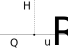
\includegraphics[scale=0.5]{QHuR} \hspace{2cm}%
$Y_Q+Y_H=Y_u\to\displaystyle{\frac{1}{6}+\frac{1}{2}=\frac{2}{3}}$



\end{frame}




\section{Dark sectors}
%A model of electroweak baryogenesis requiring no fine
%tuning and consistent to scales far above 1 TeV is
%demonstrated, in which dark matter plays the leading
%role in creating a CP asymmetry that is the source of
%the baryon asymmetry.

\begin{frame}
\begin{picture}(320,250)
\only<1->{\put(-24,-22){\begin{overpic}[scale=0.352]{z2_bkg}\end{overpic}}}%
\only<1>{\put(194,92){\begin{overpic}[scale=0.2]{infinity}\end{overpic}}}%
\only<1->{\put(30,160.5){ $\mathbf{SM}$  }}%
\only<1->{\put(18,115){\begin{overpic}[scale=0.118]{smfp}\end{overpic}}}%
\only<2>{\put(204,158){ \begin{overpic}[scale=0.27]{dfdz}\end{overpic}}}%
% \only<2>{\put(224,195){ {\huge \only<2>{
%         \hspace{0.4cm}\begin{minipage}{3cm}
%                     Hidden \\
%           QED
%         \end{minipage}
%       }}  }}%
\only<3->{\put(260,200){\Large $\color{red}\mathcal{L}=-\frac{1}{4}V_{\mu\nu}V^{\mu\nu}+\color{blue}i \sum_i{\chi_i}^\dagger\cancel{\mathcal{D}} \chi_i$   }}%
\only<3->{\put(280,180){\Large $\color{blue} - \only<3-5>{h}\only<6->{y} \left(\chi_1\chi_2 \only<3-5>{\Phi}\only<6>{S} + \text{h.c} \right) $   }}%
\only<3->{\put(280,218.5){ \Huge {{\color{red}Local}} $\color{red}U(1)_{\mathcal{X}}$  }}%
\only<3->{\put(240,125){
    \begin{minipage}{0.4\linewidth}
      Anomalons: SM-singlet Dirac fermion\\
      \only<3-5>{dark matter $\color{red}m_{\Psi}=h\langle \Phi \rangle$}\only<6>{$CP$ violation Yukawa $\color{blue}y$}
      
          {\color{red}LHC production: }
          \begin{align*}
            \text{Gauged Symmetry: $\color{red}\mathcal{X}\to B$: }&\color{red} q\overline{q}\to Z'\to \text{jets} \\
            \text{Gauged Symmetry: $\color{blue}\mathcal{X}\to L$: }&
          \end{align*}
    \end{minipage}
  }}%
\only<3->{\put(160,120){\Large $F_{\mu\nu}{\color{red}\ V^{\mu\nu}} $   }}%
\only<3->{\put(120,-10){$\color{red}\overline{\Psi}\Psi=\color{blue}\chi_1\chi_2+\chi_1^\dagger\chi_2^\dagger\to \chi_\alpha\chi_\beta \Phi^{(*)}\,,\qquad \alpha=1,\ldots N'\to N'>4 $}}
\only<3->{\put(204,0){ \begin{overpic}[scale=0.2]{tcdm1}\end{overpic}}}%

\only<4->{\put(280,0){ \begin{overpic}[scale=0.27]{alert}\end{overpic}}}%
\only<4->{\put(296,40){ {\huge 
        \hspace{0.4cm}\begin{minipage}{3cm}
          \small multi-component\\

          \vspace{-0.4cm}
          dark matter
        \end{minipage}
      }  }}%
\end{picture}
\end{frame}

\begin{frame}
  \frametitle{Standard model extended with $\operatorname{U}(1)_{\mathcal{X}={\color{cyan}L}\text{~or~}\color{red}B}$ gauge symmetry}
  \small
  \begin{table}
    \centering
        \rowcolors{1}{RoyalBlue!20}{}
  \begin{tabular}{c|c|c|c}
    \hline  
    Fields     & $\operatorname{SU}(2)_L$ & $\operatorname{U}(1)_Y $ & $\operatorname{U}(1)_{\mathcal{X}={\color{red}B}\text{ or } {\color{blue}L}}$\\ \hline
$Q^\dagger_i $    & $\boldsymbol{2}$& $-1/6$  &  $\color{red}Q$   \\
$d_{Ri} $  & $\boldsymbol{1}$& $-1/2$  &  $\color{red}d$ \\
 $u_{Ri} $  & $\boldsymbol{1}$& $+2/3$  &  $\color{red}u$\\
$L^\dagger_i $    & $\boldsymbol{2}$& $+1/2$  &  $\color{blue}L$ \\    
$e_{Ri} $  & $\boldsymbol{1}$& $-1$    &  $\color{blue} e$   \\
$H $    & $\boldsymbol{2}$& $1/2$  &  $h=0$   \\\hline
$\chi_\alpha $ & $\boldsymbol{1}$& $0$     &  $z_\alpha$   \\\hline
 $\left(L'_L\right)^\dagger$      & $\mathbf{2}$ & $1/2$   & $-x'$   \\ 
$L''_R$      & $\mathbf{2}$ & $-1/2$   & $x''$   \\ 
$e'_R$      & $\mathbf{1}$ & $-1$   & $x'$   \\ 
$\left(e''_L\right)^\dagger$      & $\mathbf{1}$ & $1$   & $-x''$   \\\hline
$\Phi$      & $\mathbf{1}$ & $0$   & $\phi$\\
$S$      & $\mathbf{1}$ & $0$   & $s$\\
  \end{tabular}
  \caption{ A minimal set of
new fermion content: $\color{blue}L=e=0$ for $\mathcal{X}=\color{red}B$. Or $\color{red}Q=u=d=0$ for $\mathcal{X}=\color{blue}L$. $i=1,2,3$, $\alpha=1,2,\ldots,N'$  }
    \label{tab:partcont2}
\end{table}
\end{frame}

\begin{frame}
  \frametitle{Effective Dirac neutrino mass operator}
\begin{align}
    \chi_1\to \nu_{R1},\cdots, \chi_{N_\nu}\to \nu_{R\, N_\nu},\qquad 2\le N_\nu\le 3\,,
\end{align}

  \begin{align*} 
    \mathcal{L}_{\text{eff}} = h_{\nu}^{\alpha i} \, \left( \nu_{R\alpha}\right)^{\dagger} \, \epsilon_{ab} \, {\color{blue} L_i^a }\, H^b \left(\frac{\Phi^*}{\Lambda}\right)^\delta + \text{H.c.},\qquad \text{with $i=1,2,3$}\,,
\end{align*}
$S$ is the complex singlet scalar responsible for the SSB of the anomaly-free gauge symmetry with $D$ or $X$-charge 
\begin{align}
     \label{eq:effcon}
    \phi=-(\nu+{\color{blue}L})/\delta\,,
\end{align}

\end{frame}



\begin{frame}
  \frametitle{Anomaly cancellation I}
The anomaly-cancellation conditions on $\left[\operatorname{SU}(3)_c\right]^{2}  \operatorname{U}(1)_{X}$, $\left[\operatorname{SU}(2)_{L}\right]^{2} \operatorname{U}(1)_{X}$, $\left[\operatorname{U}(1)_{Y}\right]^{2} \operatorname{U}(1)_{X}$,  allow us to express three of the $X$-charges in terms of the others
\begin{align}\label{eq:sol0}
  \color{red}u=&-{\color{blue}e}-\frac23 {\color{blue}L}-\frac19\left(x'-x''\right)\,,& 
\color{red}  d=& {\color{blue}e}+\frac43 {\color{blue}L}-\frac19\left(x'-x''\right)\,,& 
\color{red}  Q=& -\frac13 {\color{blue}L}+\frac19\left(x'-x''\right)\,,
\end{align}
 while the $\left[\operatorname{U}(1)_{X}\right]^{2} \operatorname{U}(1)_{Y}$ anomaly condition reduces to
 \begin{align}
     {\color{blue}(e+L)}(x'-x'')=0\,.
 \end{align}
 \vspace{-1cm}
 \begin{itemize}
 \item Previously: $x'=x''$
 \item We choose instead ($h=0$):
\begin{align}
\label{eq:emL}
    \color{blue}e=-L\,,
\end{align}
 \end{itemize}

so that ($\color{blue}L$ is still a {\color{blue}free parameter}) 
\begin{align}
\label{eq:Q}
    {\color{red}Q=-u=-d}=-\frac13 {\color{blue}L}+\frac19\left(x'-x''\right).
\end{align}
If $\color{red}B=0$ $\to \operatorname{U}(1)_{\color{blue}L}$
\end{frame}



%%%%%%%%%%%%%%%
\begin{frame}
  \frametitle{Anomaly cancellation II}
The gravitational anomaly, $\left[\operatorname{SO}(1,3)\right]^2\operatorname{U}(1)_Y$, and the cubic anomaly, $\left[\operatorname{U}(1)_X\right]^3$,
can be written as the following system of Diophantine equations, respectively,
\begin{align}
    \label{eq:Dcoond}
    \sum_{\alpha=1}^N z_\alpha=&0\,,&
    \sum_{\alpha=1}^N z_\alpha^3=&0\,,
\end{align}
%
where $N=N'+5$ and
\begin{align}
\label{eq:Nalpha}
    z_{N'+1}=&-x'\,, &&& z_{N'+2}=&x''\,,\nonumber\\
   & &\color{blue}z_{N'+2+i}&\color{blue}=L\,,\quad i=1,2,3&&
\end{align}
$\to$
\begin{align}
\label{eq:Qzero}
    9Q=-\sum_{\alpha=N'+1}^{N'+5}z_\alpha=-x'+x''\color{blue}+L+L+L\,,
\end{align}
$\color{red}Q=0$ $\cancel{\to}$ $\operatorname{U(1)}_{\color{blue}L}$
\end{frame}

%%%%%%%%%%%%%%%

%%%%%%%%%%%%%%%%%%%%%%



% \begin{frame}%[fragile,allowframebreaks]
% \frametitle{Explain also small neutrino masses }
%   In the following discussion we use the following doublets 
% \begin{align}
%   H=&
%   \begin{pmatrix}
%     H^+\\
%     H^0
%   \end{pmatrix},&
%   L_i=&
%   \begin{pmatrix}
%     \nu_{Li}\\
%     e_{Li}^{-}
%   \end{pmatrix}.
% \end{align}
% corresponding to the Higgs doublet and the lepton doublets (in Weyl Notation) respectively, such that
% \begin{align*}
%   L_i\cdot H=&\epsilon_{ab}L_i^a H^b\,,& a,b=&1,2
% \end{align*}

% \end{frame}

{
\usebackgroundtemplate{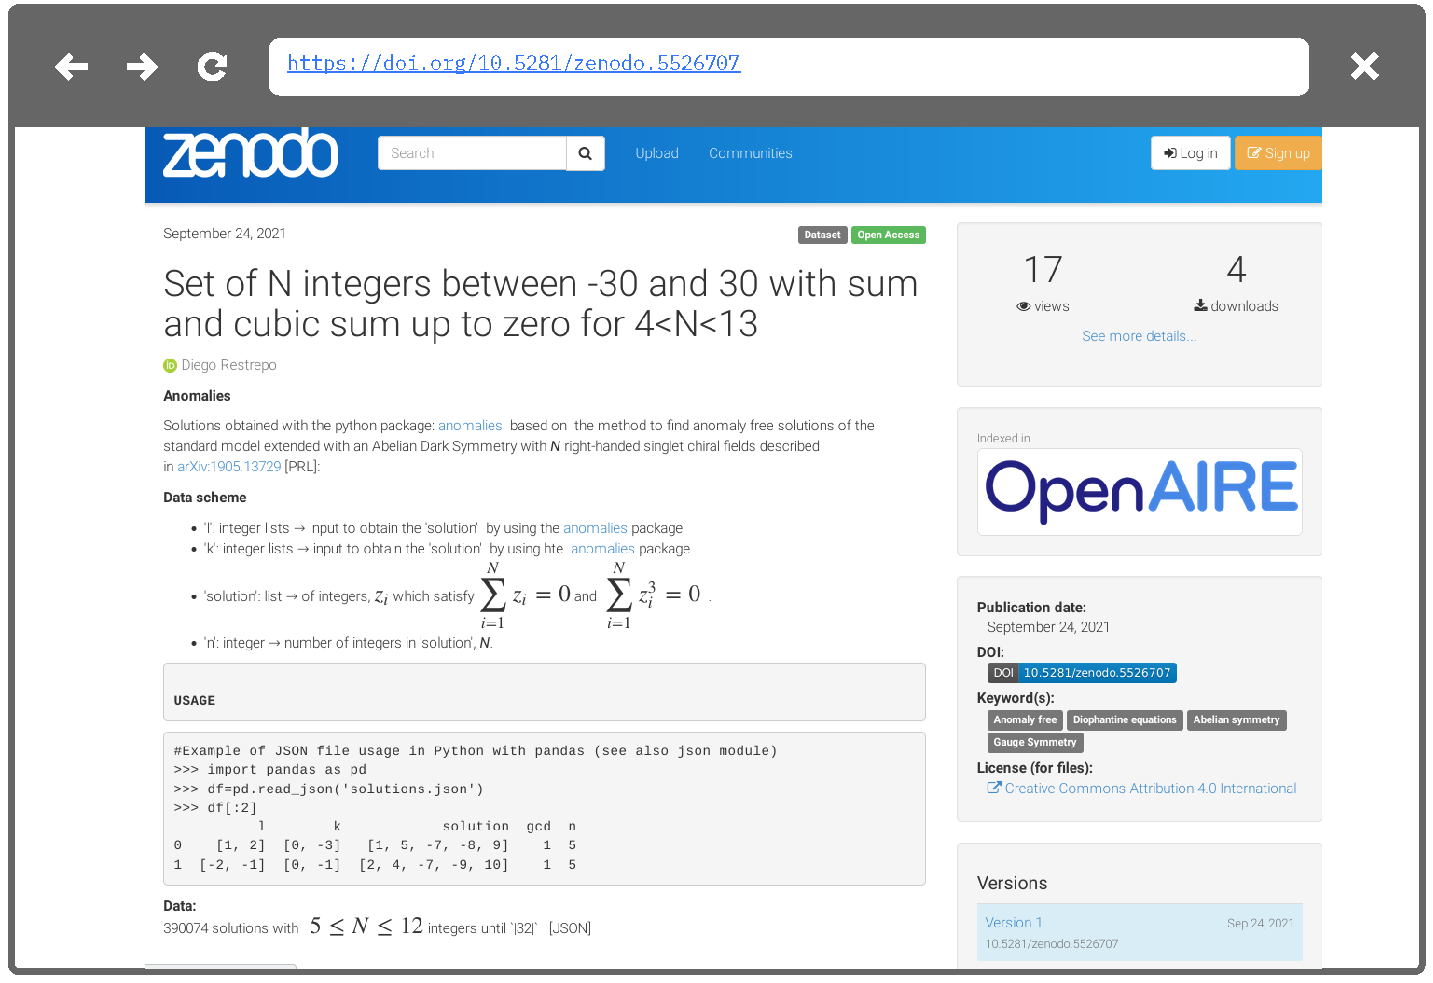
\includegraphics[width=0.8\paperwidth]{ano4}}
\setbeamertemplate{blocks}[rounded][shadow=false]
\setbeamercovered{invisible}
\begin{frame}[plain]
\begin{picture}(320,250)  
  \put(0,-7){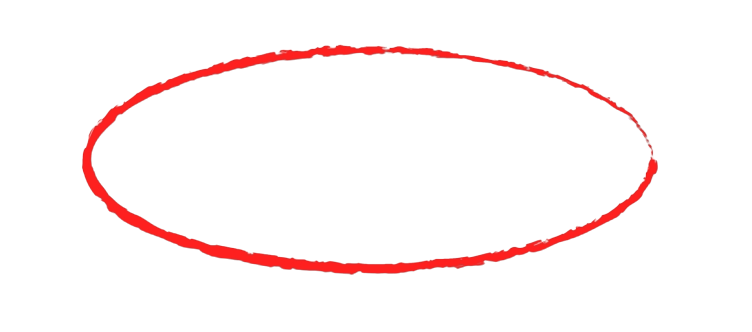
\includegraphics[scale=0.1]{encircle}}
\end{picture}
\end{frame}
%%%%%%%%%%%%%%%%%%
}


\begin{frame}
    \frametitle{$\operatorname{U}(1)_{\color{red}B}$ selection}

      \begin{columns}
    \begin{column}{0.7\textwidth}
      \begin{itemize}
      \item<1-> $\color{blue}L=0$
      \item<2-> Effective neutrino mass: $\only<2>{\color{red}}\phi=-\nu=-5$
      \item<3-> Electroweak-scale vector-like fermions: $\only<3>{\color{red}}\left(L_L'\right)^\dagger L_R''\Phi^*\to x'=-1,\ x''=6$
      \item<4-> Dirac-fermionic DM: $\only<4>{\color{red}}\left(\chi_L\right)^\dagger \chi_R''\Phi^*\to z_3=-3,\ z_4=-2$
      \end{itemize}
    \end{column}
    \begin{column}{0.3\textwidth}
      \vspace{1cm}
      
      \Large $({\only<1->{\color{black}}\only<2>{\color{red}}5, 5},
      {\only<1->{\color{black}}\only<4>{\color{red}}-3, -2},
      {\only<1->{\color{black}}\only<3>{\color{red}}1, -6})$


    %\hfill  \tiny{\url{Dreamstime.com}}  
    \end{column}

  \end{columns}

  \invisible<1-4>{\only<5>{{\color{red}959} solutions from $\sim 400,000$}}

  \invisible<1-4>{
    \begin{minipage}[t]{3.0\linewidth}
      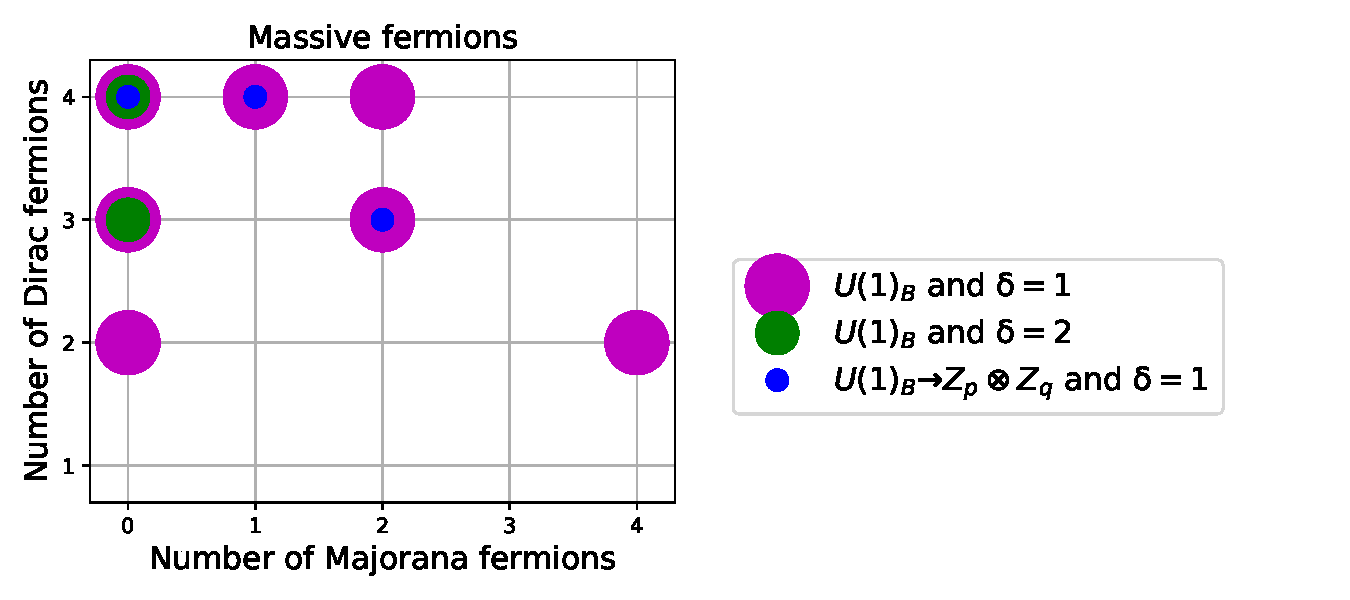
\includegraphics[scale=0.45]{number}\hspace{0.5cm}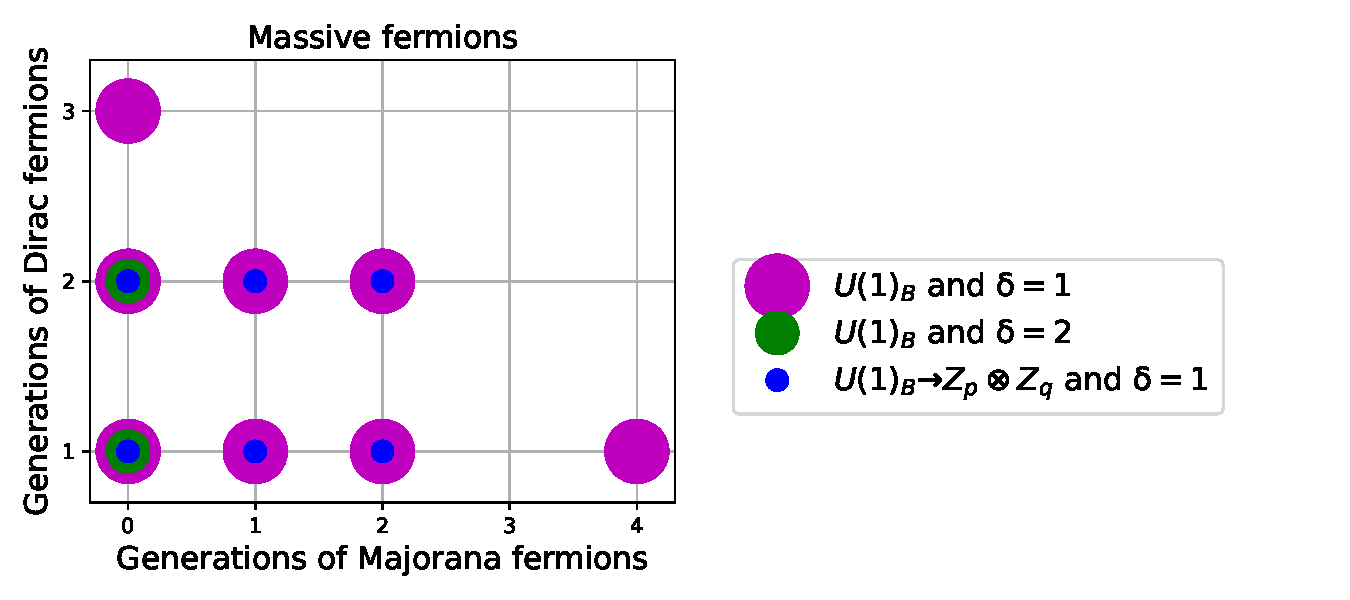
\includegraphics[scale=0.45]{generation}
    \end{minipage}
  }

  \end{frame}


\begin{frame}
  \frametitle{Scotogenic realization}
  Any realization which does not affect anomaly cancellation is allowed

  \begin{columns}
    \begin{column}{0.6\textwidth}
\only<1>{  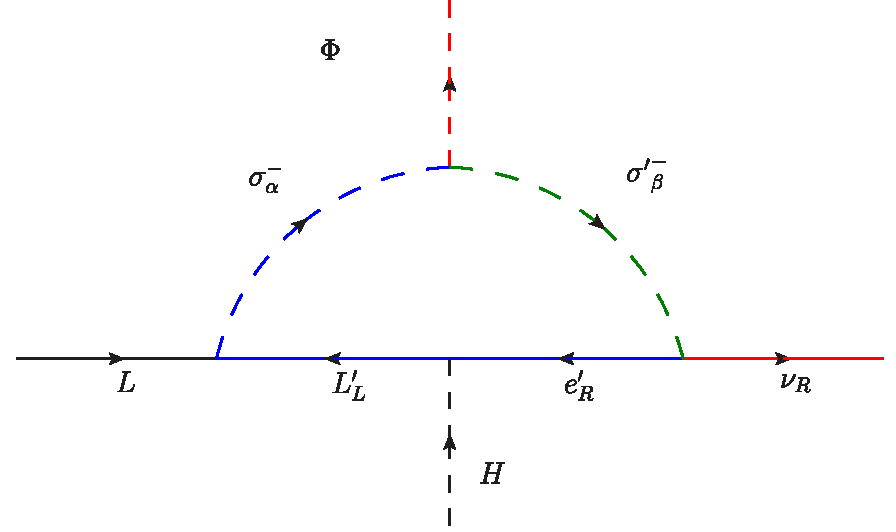
\includegraphics[scale=0.6]{zee1}      }%
\only<2-3>{  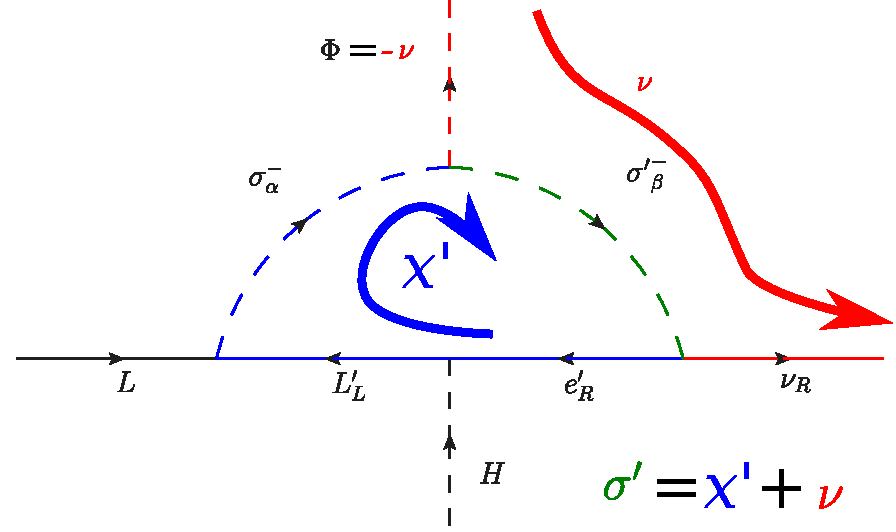
\includegraphics[scale=0.6]{zee2}      }%
\end{column}
    \begin{column}{0.4\textwidth}
      % \hfill  \tiny{\url{Dreamstime.com}}
      \invisible<1-2>{
        \centering
        \scriptsize
        \rowcolors{1}{RoyalBlue!20}{}
  \begin{tabular}{l|c|c|c}\hline
    Field&$SU(2)_L$ & $U(1)_Y$&$\operatorname{U}(1)_B$\\\hline
     $u_{Ri}$      & $\mathbf{1}$ & $2/3$   & $u=1/3$   \\ 
     $d_{Ri}$      & $\mathbf{1}$ & $-1/3$   & $d=1/3$   \\ 
     $\left(Q_i\right)^\dagger$      & $\mathbf{2}$ & $-1/6$   & $Q=-1/3$   \\ 
     $\left(L_i\right)^\dagger$      & $\mathbf{2}$ & $1/2$   & $L=0$   \\ 
     $e_R$      & $\mathbf{1}$ & $-1$   & $e=0$   \\ 
     $\color{blue}\left(L'_L\right)^\dagger$      & $\color{blue}\mathbf{2}$ & $\color{blue}1/2$   & $\color{blue}-x'=-3/5$   \\ 
     $\color{blue}e'_R$      & $\color{blue}\mathbf{1}$ & $\color{blue}-1$   & $\color{blue}x'=3/5$   \\ 
     $L''_R$      & $\mathbf{2}$ & $-1/2$   & $x''=18/5$   \\ 
     $\left(e''_L\right)^\dagger$      & $\mathbf{1}$ & $1$   & $-x''=-18/5$   \\ 
     $\color{red}\nu_{R,1}$   & $\color{red}\mathbf{1}$ & $\color{red}0$   & $\color{red}-3$   \\
     $\color{red}\nu_{R,2}$   & $\color{red}\mathbf{1}$ & $\color{red}0$   & $\color{red}-3$   \\
     $\chi_{R}$      & $\mathbf{1}$ & $0$   & $6/5$   \\
     $\left(\chi_{L}\right)^\dagger$      & $\mathbf{1}$ & $0$   & $9/5$   \\ \hline
     $H$      & $\mathbf{2}$ & $1/2$   & $0$   \\
     $S$      & $\mathbf{1}$ & $0$   & $3$   \\
     $\color{red}\Phi$      & $\color{red}\mathbf{1}$ & $\color{red}0$   & $\color{red}3$   \\
     $\color{blue}{\sigma}^-_\alpha$      & $\color{blue}\mathbf{1}$ & $\color{blue}1$   & $\color{blue}3/5$   \\
     $\color{Green}{\sigma'}^-_\alpha$      & $\color{Green}\mathbf{1}$ & $\color{Green}-1$   & $\color{Green}-12/5$   \\
     \hline
  \end{tabular}
        }
    \end{column}
  \end{columns}

  

\end{frame}


% \section{Baryogenesis}
\section{Electroweak baryogenesis}
\begin{frame}
  \frametitle{Problems}
  \begin{itemize}
%check: coloremoji/emoji_images/hires/
\item Standard model (SM)  $m_h\sim 40\text{~GeV}$. 
\includegraphics{1F61E}
\item Beyond the SM: Source of CP contains fields charged under SM\\ $\to$ too large electric dipole moments 
\includegraphics{1F629}
\end{itemize}
\end{frame}


\begin{frame}
  \frametitle{Dark sectors}
\begin{itemize}
\item Inert SM-singlet complex scalar field which acquires vev with temperature to have strong electroweak phase transition 
\includegraphics{1F60A}
\item CP violation (CPV) triggered in dark sectors through SM gauge singlets\\
  $\to$ CPV Yukawa between SM-singlet complex scalar and SM-singlet quiral fermions 
\includegraphics{1F600}
\end{itemize}
  
\end{frame}

\begin{frame}
  \only<1>{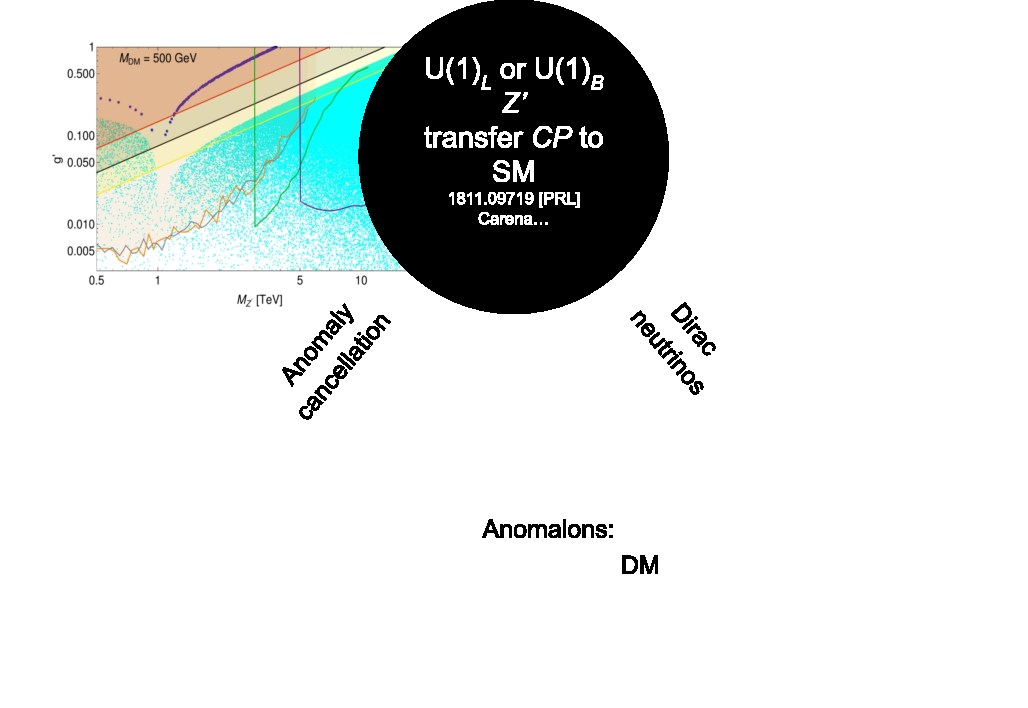
\includegraphics[scale=0.8]{triangle1}}
  \only<2>{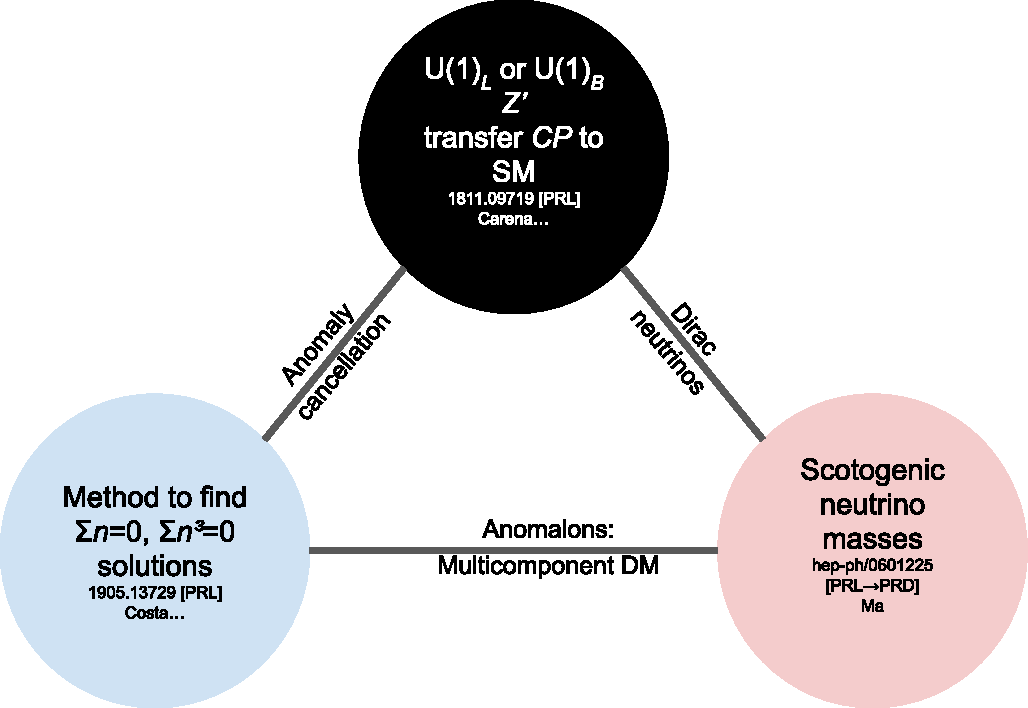
\includegraphics[scale=0.8]{triangle2}}
\end{frame}
  

%%missing here




\begin{frame}
  \frametitle{Dark sector baryogenesis}
  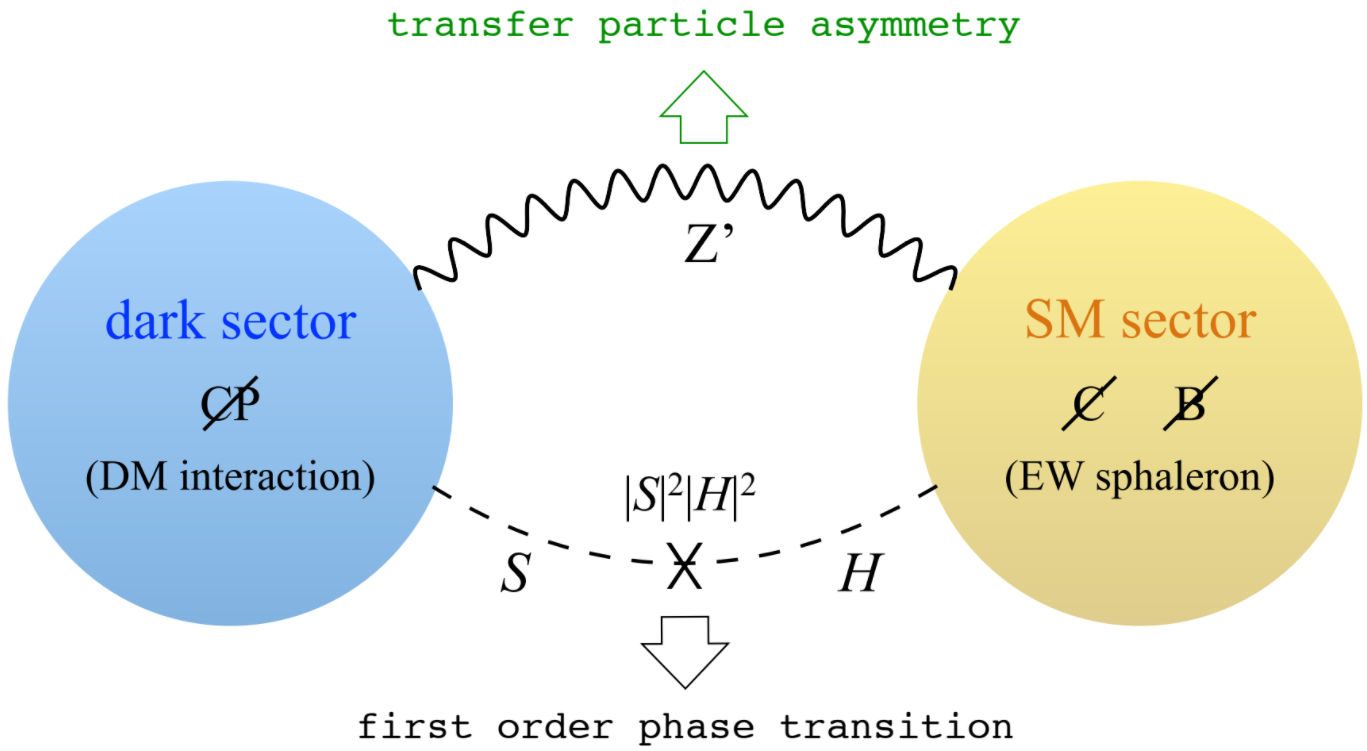
\includegraphics[scale=0.55]{new-baryogenesis}

  \begin{flushright}
      \tiny{from: [1] Carena, \emph{et al}, arXiv:1908.04818 [PRD] (see also: arXiv:1811.09719 [PRL]) }
  \end{flushright}
\end{frame}

\begin{frame}
  \frametitle{Baryogenesis}
  CP violation occurs in the dark sector and is transmited to SM sector by the new $Z'$ gauge boson.

  \begin{itemize}
  \item   High scale fields:
  $
  \Phi\,,\qquad  \left( \langle\Phi\rangle \to L'_L, L''_R,e'_L,e''_R\text{:~ EW-scale vector-like anomalons}\right) 
  $
  
  
\item Electroweak scale (EW) fields:
  \fcolorbox{red}{yellow}{ $ Z'_\mu, S, \chi_L,\chi_R $}
\item $CP$-violation 
    \begin{align*}
      \mathcal{L}_{\text{Dirac DM}}=&h \left(\chi_L\right)^\dagger \chi_R \Phi^* + {\color{red} y \left(\chi_L\right)^\dagger \chi_R S^*}+\text{h.c}\,,& {\color{red}y}\in&\mathbb{C}\\
      \supset& \left( m_{\chi} + {\color{red}|y| \operatorname{e}^{i\theta}|S|} \right)\left(\chi_L\right)^\dagger \chi_R+\text{h.c}\,.&&
  \end{align*}
  \item $CP$-violation Portal
    \begin{align*}
\mathcal{L}_{\text{anomalous}} \supset g^{\prime} Z_{\mu}^{\prime}\left[3 \bar{\chi}_{L} \gamma^{\mu} \chi_{L}-2\bar{\chi}_{R} \gamma^{\mu} \chi_{R}+\bar{Q}_{i} \gamma^{\mu} Q_{i}+\bar{q}_{Ri} \gamma^{\mu} q_{Ri}\right]
    \end{align*}
  \item Strong electroweak phase transition (EWPT) portal
    \begin{align*}
      \mathcal{L}_{\text{first order EWPT}}\supset -\lambda_{S H} H^{\dagger}H\, S^{*}S\,.
    \end{align*}
  \end{itemize}

\end{frame}

\begin{frame}
  \frametitle{First-order phase transition: Effective potential ($T\ne 0$)}
\fcolorbox{red}{yellow}{  $h=H/\sqrt{2}$, $s=|S|$ } with vevs: $v(T)$ and $w(T)$ such that $v(T_c)=w(T_c)$
\begin{align}
   V_T(h,s)\,=\,& \frac{\lambda_H v_c^4}{4}\left(\frac{h^2}{v_c^2} +\frac{s^2}{w_c^2} -1\right)^2 + \frac{\lambda_H v_c^2}{m_{s,c}^2 w_{0,c}^4}h^2 s^2 
     + (T^2-T_c^2)(c_h h^2 +c_s s^2)\,, %+ {\color{red} \frac{1}{12}T^2 \lambda\, m_\chi\, } S,
\end{align}
where
\begin{align}
    c_h\,=\,&\frac{1}{48} \left(9g_2^2+ 3g_1^2 +12 y_t^2 +24 \lambda_H +\lambda_{HS}\right)\, ,\quad
    c_s\,=\,  \frac{1}{12} \left (3 \lambda_S + 2 \lambda_{HS} \right)\,. 
\end{align} 
\vspace{-0.4cm}
\begin{columns}
  \begin{column}{0.5\textwidth}
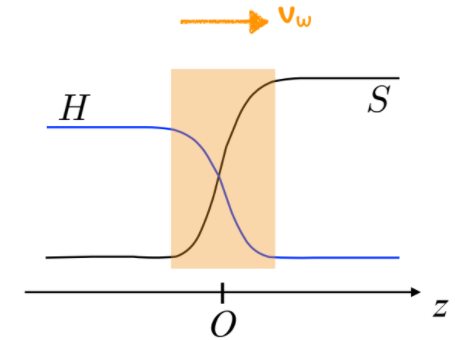
\includegraphics[scale=0.6]{bubble}    
  \end{column}
  \begin{column}{0.5\textwidth}
\invisible<1>{\tiny arXiv: Sec.~4.1 arXiv:1107.5451 }
\invisible<1>{\only<2>{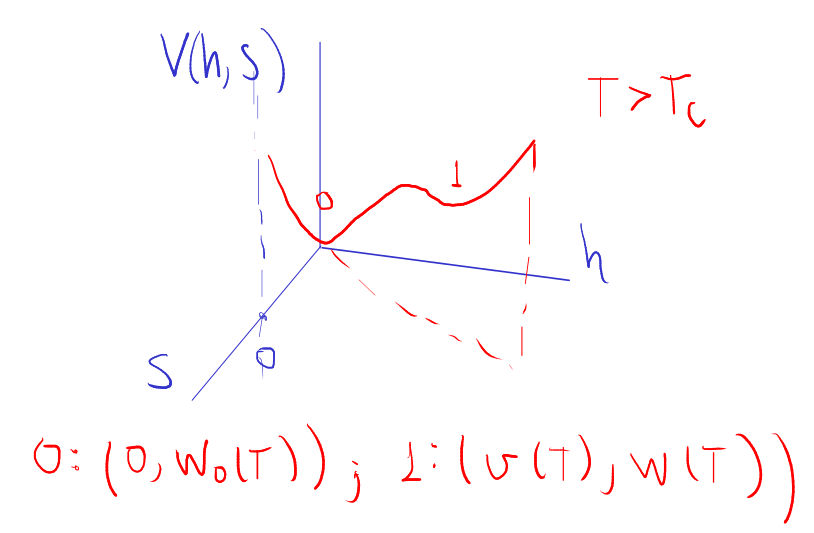
\includegraphics[scale=0.5]{v1}}%
\only<3>{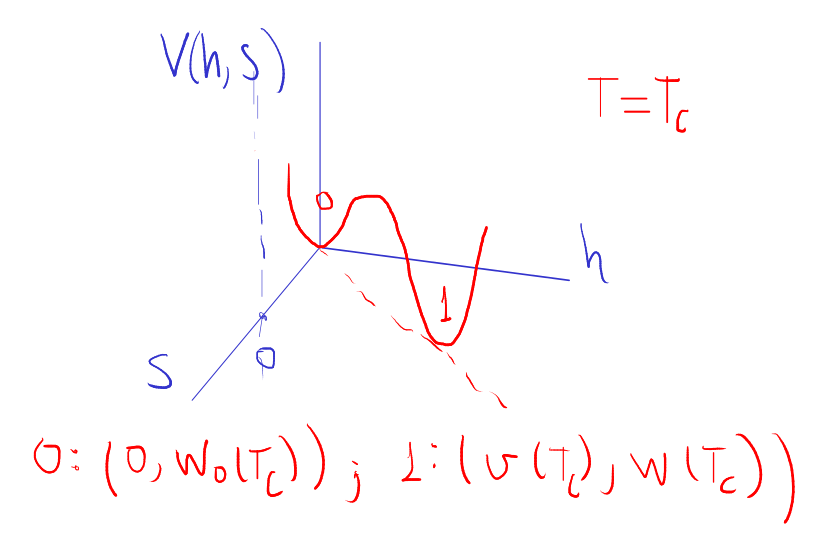
\includegraphics[scale=0.5]{v2}}%
\only<4>{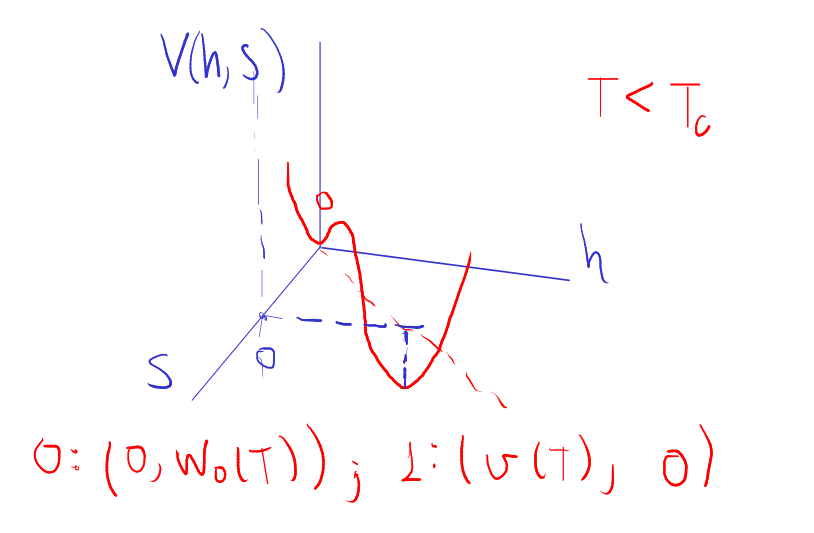
\includegraphics[scale=0.5]{v3}}%
      }
  \end{column}
\end{columns}


\end{frame}
\begin{frame}[fragile,allowframebreaks]
\frametitle{$CP$ assymetry generation}


 Using the thin wall approximantion for the nucleation bubbles,
  we use the ansatz in which the space dependence of the fields is given by 
\begin{equation*}
    h(z) \,=\, \frac{1}{2}v(T_n) \left(1- \tanh \left(z/L_w \right) \right)\,,\qquad
    s(z) \,=\, \frac{1}{2}w_0(T_n) \left(1+ \tanh \left(z/L_w \right) \right)\,, 
\end{equation*}  
where $z$ is the direction normal to the wall and $L_w$ is the wall width.

%\newpage{}
The nucleation temperature, $T_n$, is defined by the condition
\begin{equation*}
    \exp \left (-S_3 /T_n \right) \,=\, \frac{3}{4\pi}\left(\frac{H(T_n)}{T_n} \right)^4 \left(\frac{2\pi\,T_n}{S_3}\right)^{\frac{3}{2}} \,,
\end{equation*}
 where $S_3$ is the Euclidean action of the bubble and $H(T)$ is the Hubble rate.



\end{frame}

\begin{frame}[fragile,allowframebreaks]
\frametitle{Boltzmann equation}
 $\xi_i(z)\,\equiv\,{\mu_i(z)}/{T} \,=\,{6}\left(n_i - \overline{n}_{i} \right)/{T^3}$,
\begin{equation*}
- D_L \xi''_{\chi_L} -v_w\xi'_{\chi_L} +\Gamma_L(\xi_{\chi_L}-\xi_{\chi_R})\,=\,S_{\cancel{CP}}\,,
\end{equation*}
where $D_L$ is the diffusion constant for $\chi_L$, which is related to the scattering rate $\Gamma_L$ by
\begin{align}
  D_L= \frac{3x+2}{x^2 +3x+2}\frac{1}{3\Gamma_L}, \qquad\qquad x\equiv m_\chi /T\,
\end{align}
 and
\begin{align}
  S_{\cancel{CP}}\,=\,-\frac{\lambda}{2}\frac{v_w D_L}{\frac{3x+2}{x^2 +3x+2} T} \frac{(1-x)e^{-x} + x^2 E_1(x) }{4m_\chi^2 K_2(x)}
  \frac{m_\chi w_0(T_n) \lambda \left(-2+\cosh \left(\frac{2z}{L_w} \right) \right)\sin \theta}{L_w^3 \cosh^4 \left(\frac{z}{L_w} \right)}\,,
\end{align}
where $v_w$ is the wall's velocity 
$E_1(x)$ is the error function and $K_2(x)$ is the modified Bessel function of the second kind. ${\color{red}y}=\lambda\operatorname{e}^{i\theta -i\pi/2}$

\end{frame}


\begin{frame}
\frametitle{Transfer DM assymetry to SM quarks}
The chiral particle give rise to a non-zero $\operatorname{U}(1)_B$ charge density in the proximity of the wall. This results in a $Z'$ background that couples to the SM fields with $\operatorname{U}(1)_B$ charge,
\begin{equation*}
    \langle Z'_0(z) \rangle \,=\, \frac{ g_B\,(q_{\chi_L}-q_{\chi_R})T_n^3}{6 M_{Z'}} \int_{-\infty}^\infty \operatorname{d}z_1\, \xi_{\chi_L}(z_1)\, e^{-M_{Z'}|z-z_1|}\, , 
\end{equation*} which generates a chemical potential for the SM quarks, 
\begin{equation*}
\mu_{Q}(z)\,=\, \mu_{d_R,u_R}(z)\,=\, 3 \times \frac{5}{9} \times g_B \langle Z'_0 (z) \rangle. 
\end{equation*} 
This chemical potential sources a thermal-equilibrium asymmetry in the quarks, $ \Delta n_{Q}^{\rm EQ} (z) \,\sim \, T_n^2 \, \mu_{Q}(z)$. 

From [1]
\begin{quote}
\fcolorbox{red}{yellow}{If the $Z'$ is sufficiently
light, it mediates a long range force that extends into the region }
\fcolorbox{red}{yellow}{ outside the bubble wall with
unbroken electroweak symmetry. }

\end{quote}

\end{frame}
\begin{frame}
  \frametitle{Finally, the baryon-number asymmetry is then given by}

\begin{equation*}
  n_B\,=\,  \frac{\Gamma_{\rm sph}}{v_w} \int_0^{\infty}\operatorname{d}z\, n_{Q}^{\rm EQ} (z)\, \exp\left(-\frac{\Gamma_{\rm sph}}{v_w}\,z\right)\,,
\end{equation*} 
where $\Gamma_{\rm sph}$ is the sphaleron rate. The baryon-to-photon-number ratio is then obtained by
\begin{equation*}
 \eta_B \,=\, \frac{n_B}{s(T_n)},\quad s (T) \,\equiv\,\frac{2\pi^2}{45} g_{*S}(T)\, T^3\,, 
\end{equation*} where $g_{*S}(T)$ is the effective number of relativistic degrees of freedom.

Our goal is to find what regions of the parameter space yield
%
\begin{align}
\label{eq:eta-value}
0.82\times 10^{-10} < \eta_B < 0.92\times 10^{-10}\,.
\end{align}


\end{frame}

\begin{frame}
  \frametitle{https://github.com/anferivera/DarkBariogenesis}

  \begin{itemize}
  \item   SARAH$\to$SPheno$\to$MicroMegas
    
  \item  $\eta_B$ calculation code
  \item Python notebook with the scan 
  \end{itemize}

  \begin{block}{arXiv:1810.08055}
\textbf{Ten Simple Rules for Reproducible Research in Jupyter Notebook}
Fernando Pérez,\emph{et al} 

[...] In this paper, we address several questions about reproducibility
[...]
Combined with software repositories and open source licensing, notebooks are powerful tools for transparent, collaborative, reproducible, and reusable data analyses.
  \end{block}


  
\end{frame}




\begin{frame}
  \frametitle{Results}
  We vary the typical Dirac-fermion DM parameter space and for each point that satisfy neutrino oscillation data, relic density and DM direct detection constraints. For each point  we ... 
  
  \begin{table}[t]
\centering
\begin{tabular}{c|c} 
\hline
Parameter & Range\\
\hline
$\theta$ & $(-\pi/2 \,, \pi/2)$  \\
$w_0(T_n)/{\rm GeV} $ &  $100-500$\\
$T_n/{\rm GeV}$ &  $100-200$\\
$L_w /{\rm GeV^{-1}}$ &  $1/T_n - 10/T_n$\\
$v_w$ &  $0.05 - 0.5$\\
\hline
\end{tabular}
\caption{Scan ranges for the free parameters that are involved in the baryogenesis mechanism.}
\label{tab:scan-baryogenesis}
\end{table}
\end{frame}

\begin{frame}
  \frametitle{Black points: Dirac neutrinos with proper DM and baryon assymetry}
  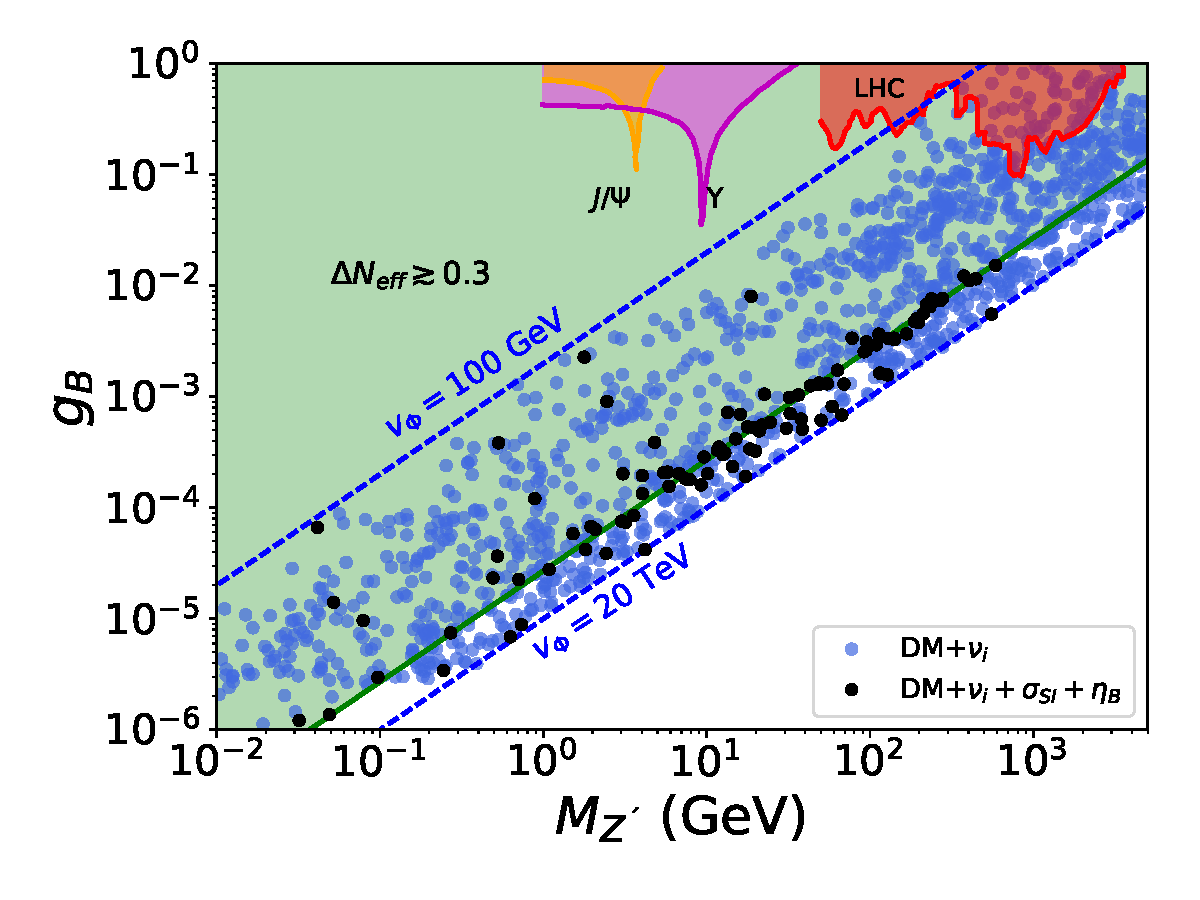
\includegraphics[scale=0.55]{g1_MZp}
\end{frame}
 
\begin{frame}
  \frametitle{Conclusions}
  A $\operatorname{U}(1)_B$ is presented as an example of models where all new fermions required to cancel out the anomalies are used to solve phenomenological problems of the standard model (SM):
  \begin{itemize}
  \item   EW-scale fermion vector-like doublets and iso-singlet charged singlets, in conjunction with right-handed neutrinos with repeated Abelian charges, participate in the generation of small neutrino masses through the Dirac-dark Zee mechanism
  \item The other SM-singlets are used to explain the dark matter in the universe, while their coupling to an inert singlet scalar is the source of the $CP$ violation.
  \end{itemize}
In the presence of a strong first-order electroweak phase transition, this ``dark'' $CP$ violation allows for successful electroweak baryogenesis by using long range force mediated by a sufficiently light $Z'$ which transfers the assymmetry from the Dark sector into the SM.
\end{frame}

\end{document}  
\begin{frame}
  \frametitle{$\operatorname{U}(1)_{\color{red}B}$ selection}

  Starting from the extended dataset with the solutions with $N$ integers to the Diophantine equations~\eqref{eq:NN3} we apply the following steps
\begin{itemize}
    \item Check that the solution has two (three) repeated integers to be identified as $\nu$ and fix $N_\nu=2$  ($N_\nu=3$).
    \item For $\delta=1,2,\ldots$ and all the possible combinations for $m$ and $\nu$ in the solution, including $m=0$, find the $s$ value compatible with the effective Dirac neutrino mass operator of D-$(4+\delta)$ according to eq.~\eqref{eq:effcon}.
    \item Interpret the integers in the solution that are different from $m$ and $\nu$ as the $D$-charges for $m=0$ or the $X$-charges for $m\ne 0$, of a set of singlet chiral fermions: $\psi_i$, $i=1,\ldots, N_{\text{chiral}}-N_{\nu}$.  Then select the solutions for which the condition 
    \begin{align}
        |n_i+n_j|=|s|,
    \end{align}
    which guarantees that all the singlet chiral fermions, $\psi_i$, acquire masses after the spontaneous symmetry breaking of the gauge Abelian symmetry through $\langle S\rangle$.
\end{itemize}
  
\end{frame}



\begin{frame}
  \begin{figure}
    \centering
    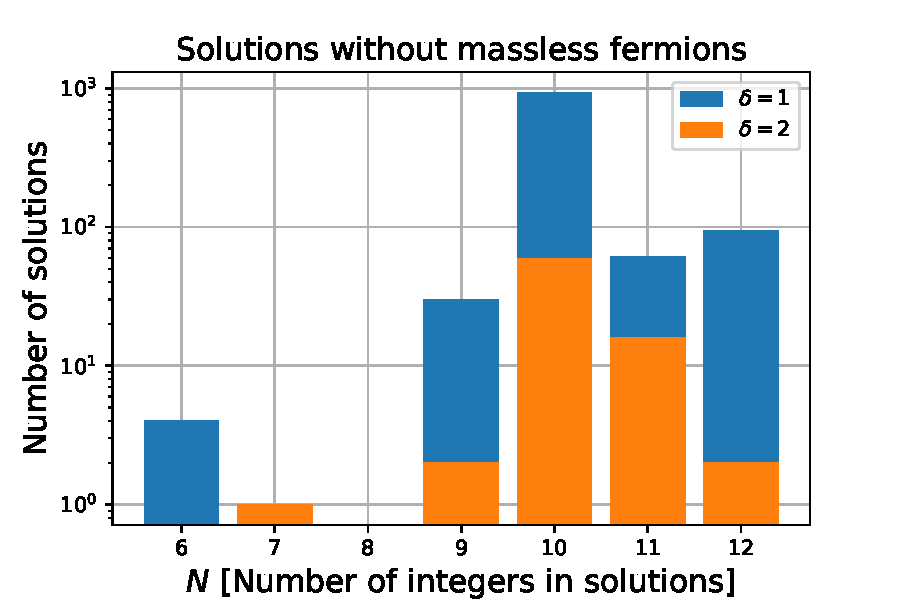
\includegraphics[scale=0.7]{solutions}
     \caption{Distribution of solutions with $N$ integers to the Diophantine equations~\eqref{eq:NN3} which allow the effective Dirac neutrino operator at D-$4+\delta$ for at least two right-handed neutrinos and have non-vanishing Dirac o Majorana masses for the other singlet chiral fermions in the solution.}
    \label{fig:solutions}
\end{figure}
\end{frame}

\begin{frame}
  \frametitle{48 type of representative solutions}
%  \begin{table}
%    \centering
{
  \begin{tiny}
  \begin{tabular}{L|RC|RRR|R|RRRR}
\toprule
                                           \text{Solution} & N &N_{\text{chiral}} &   m & \nu & \delta &                s  & N_D & N_M & G_D & G_M \\
\midrule
                              (1, -2, -3, 5, 5, -6) &  6 &  6 &   0 &   5 &      1 &               -5 &   2 &   0 &   1 &   0 \\
                           (3, 3, 3, -5, -5, -7, 8) &  7 &  4 &   3 &  -5 &      2 &                1 &   1 &   0 &   1 &   0 \\
                    (1, -2, 3, 4, 6, -7, -7, -7, 9) &  9 &  9 &   0 &  -7 &      1 &                7 &   3 &   0 &   1 &   0 \\
                  (1, 1, -4, -5, 9, 9, 9, -10, -10) &  9 &  9 &   0 &   9 &      1 &               -9 &   3 &   0 &   2 &   0 \\
                   (1, 2, -6, -6, -6, 8, 9, 9, -11) &  9 &  6 &  -6 &   9 &      1 &               -3 &   2 &   0 &   1 &   0 \\
                (1, -3, 8, 8, 8, -12, -12, -17, 19) &  9 &  6 &   8 & -12 &      2 &                2 &   2 &   1 &   1 &   1 \\
              (8, 8, 8, -12, -12, 15, -17, -23, 25) &  9 &  6 &   8 & -12 &      2 &                2 &   2 &   0 &   1 &   0 \\
                (1, -2, -2, 3, 3, -4, -4, 6, 6, -7) & 10 & 10 &   0 &   6 &      1 &               -6 &   3 &   2 &   2 &   2 \\
                (1, -2, -2, 3, 4, -5, -5, 7, 7, -8) & 10 & 10 &   0 &  -5 &      1 &   \boldsymbol{5} &   4 &   0 &   2 &   0 \\
                (1, -2, -2, 3, 5, -6, -6, 8, 8, -9) & 10 & 10 &   0 &  -6 &      1 &                6 &   4 &   0 &   2 &   0 \\
                 (2, 2, 3, 4, 4, -5, -6, -6, -7, 9) & 10 & 10 &   0 &   2 &      1 &  \boldsymbol{-2} &   4 &   2 &   2 &   2 \\
                (1, 1, 5, 5, 5, -6, -6, -6, -9, 10) & 10 & 10 &   0 &   1 &      1 &               -1 &   4 &   0 &   3 &   0 \\
               (2, 2, 4, 4, -7, -7, -9, -9, 10, 10) & 10 & 10 &   0 &  10 &      2 &               -5 &   3 &   0 &   2 &   0 \\
                (1, 2, 2, -3, 6, 6, -8, -8, -9, 11) & 10 & 10 &   0 &  -8 &      1 &                8 &   4 &   1 &   2 &   1 \\
             (1, -2, -3, 5, 6, -8, -9, 11, 11, -12) & 10 & 10 &   0 &  11 &      1 &              -11 &   4 &   0 &   1 &   0 \\
              (1, 1, -3, 4, 4, -7, 8, -10, -10, 12) & 10 & 10 &   0 & -10 &      2 &                5 &   4 &   0 &   2 &   0 \\
            (1, 1, -2, -2, -4, 6, -10, 11, 12, -13) & 10 & 10 &   0 &  -2 &      1 &                2 &   3 &   2 &   1 &   2 \\
               (3, 4, 4, 4, 4, -5, -8, -8, -11, 13) & 10 & 10 &   0 &  -8 &      1 &                8 &   2 &   4 &   1 &   4 \\
             (4, 4, 5, 6, 6, -9, -10, -10, -11, 15) & 10 & 10 &   0 &   6 &      1 &               -6 &   4 &   0 &   2 &   0 \\
           (1, -2, -4, 7, 7, -10, -12, 14, 14, -15) & 10 & 10 &   0 &  14 &      1 & \boldsymbol{-14} &   3 &   2 &   1 &   2 \\
             (1, 2, 2, -3, 4, -6, 12, -13, -14, 15) & 10 & 10 &   0 &   2 &      1 &  \boldsymbol{-2} &   4 &   1 &   1 &   1 \\
              (1, 4, 4, -7, 8, 8, -9, -12, -12, 15) & 10 & 10 &   0 &   8 &      1 &               -8 &   4 &   2 &   2 &   2 \\
            (1, 2, 2, -9, -9, 16, 16, 17, -18, -18) & 10 & 10 &   0 & -18 &      1 &               18 &   3 &   2 &   2 &   2 \\
          (1, -3, -6, 7, -10, 11, -16, 18, 18, -20) & 10 & 10 &   0 &  18 &      2 &               -9 &   4 &   0 &   1 &   0 \\
\bottomrule  
\end{tabular}
\end{tiny}
}
% \caption{
% %   Set of charges satisfying the Diophantine equations together with the conditions enumerated in the text, for solutions with $N_{\textbf{chiral}}$ massive fermions, including 
% % the Dirac neutrinos masses allowed by the effective operator of power $\delta$,
% %  the solution with unconditional stability through $\mathbb{Z}_{|s|}$ is highlighted with a bold font for the charge of $|s|=\boldsymbol{6},\boldsymbol{14}$. $N_D$ and $N_M$ are the number of massive Dirac and Majorana singlet fermions in each solution, while $G_D$ and $G_M$ are the corresponding number of maximum generations in the set.
% }
% \label{tab:sltns}
% \end{table}
\end{frame}

\begin{frame}
  \frametitle{48 type of representative solutions}
%  \begin{table}
%    \centering
{
  \begin{tiny}
  \begin{tabular}{L|RC|RRR|R|RRRR}
\toprule
                                           \text{Solution} & N &N_{\text{chiral}} &   m & \nu & \delta &                s  & N_D & N_M & G_D & G_M \\
\midrule
           (1, -4, 5, -6, -6, 10, -14, 15, 20, -21) & 10 & 10 &   0 &  -6 &      1 &                6 &   4 &   0 &   1 &   0 \\
          (2, -3, -6, 7, 12, -14, -14, 17, 20, -21) & 10 & 10 &   0 & -14 &      1 &  \boldsymbol{14} &   4 &   1 &   1 &   1 \\
             (3, 6, 6, -7, 8, 8, -14, -14, -17, 21) & 10 & 10 &   0 & -14 &      1 &  \boldsymbol{14} &   4 &   1 &   2 &   1 \\
          (8, 8, 9, 10, 10, -13, -18, -18, -27, 31) & 10 & 10 &   0 & -18 &      1 &  \boldsymbol{18} &   4 &   1 &   2 &   1 \\
             (1, 1, 1, -2, -2, -5, -5, 6, 6, 7, -8) & 11 &  8 &   1 &  -2 &      1 &                1 &   3 &   0 &   2 &   0 \\
            (1, -2, -2, -2, -3, 4, 4, -5, 6, 7, -8) & 11 &  8 &  -2 &   4 &      1 &               -2 &   3 &   1 &   1 &   1 \\
             (1, 1, 2, 2, 2, -4, -4, 7, -8, -9, 10) & 11 &  8 &   2 &  -4 &      1 &                2 &   2 &   2 &   1 &   2 \\
           (2, 2, 2, -4, -4, -5, 7, -8, 9, 10, -11) & 11 &  8 &   2 &  -4 &      1 &                2 &   3 &   0 &   1 &   0 \\
          (1, -2, -3, -3, -3, 5, 5, -7, 8, 10, -11) & 11 &  8 &  -3 &   5 &      2 &               -1 &   3 &   0 &   1 &   0 \\
            (3, 3, 3, -4, -4, 7, 7, -8, -9, -9, 11) & 11 &  8 &   3 &  -9 &      2 &                3 &   3 &   0 &   2 &   0 \\
          (1, 3, 5, -6, -6, -6, 8, -9, 12, 12, -14) & 11 &  8 &  -6 &  12 &      1 &               -6 &   3 &   1 &   1 &   1 \\
          (1, -2, 6, 6, 6, -7, 8, -9, -12, -12, 15) & 11 &  8 &   6 & -12 &      1 &   \boldsymbol{6} &   3 &   0 &   1 &   0 \\
          (1, 3, 3, 6, 6, 6, -7, -10, -12, -12, 16) & 11 &  8 &   6 & -12 &      1 &   \boldsymbol{6} &   2 &   2 &   1 &   2 \\
         (1, -2, -2, -2, 3, 3, 4, 4, -5, -5, -5, 6) & 12 &  9 &  -5 &  -2 &      1 &   \boldsymbol{7} &   3 &   0 &   2 &   0 \\
         (1, 1, -3, 4, 5, 5, 5, -6, -7, -7, -8, 10) & 12 &  9 &   5 &  -7 &      1 &                2 &   3 &   2 &   1 &   2 \\
         (1, 1, 1, -2, 4, -7, -7, -7, 8, 9, 9, -10) & 12 &  9 &  -7 &   9 &      1 &               -2 &   2 &   3 &   1 &   3 \\
        (1, 1, -3, -3, -5, -5, -5, 7, 7, 7, 9, -11) & 12 &  9 &  -5 &   7 &      1 &               -2 &   3 &   2 &   2 &   2 \\
     (1, -3, -3, -3, 4, 6, 7, 9, -10, -10, -10, 12) & 12 &  9 &  -3 & -10 &      1 &               13 &   3 &   0 &   1 &   0 \\
       (1, 1, 1, 3, 3, -5, 7, 7, -11, -11, -11, 15) & 12 &  9 &   1 & -11 &      1 &               10 &   3 &   1 &   2 &   1 \\
         (1, 1, 1, 3, 5, 5, -5, 5, -9, -9, -13, 15) & 12 &  9 &   5 &  -9 &      2 &                2 &   2 &   3 &   1 &   3 \\
  (1, -2, -2, 3, 6, -10, -10, -10, 13, 14, 14, -17) & 12 &  9 & -10 &  14 &      1 &               -4 &   4 &   2 &   2 &   2 \\
(1, -3, 9, -11, -13, -13, -13, 15, 15, 15, 21, -23) & 12 &  9 & -13 &  15 &      1 &               -2 &   3 &   1 &   1 &   1 \\
\bottomrule  
\end{tabular}
\end{tiny}
}
% \caption{
% %   Set of charges satisfying the Diophantine equations together with the conditions enumerated in the text, for solutions with $N_{\textbf{chiral}}$ massive fermions, including 
% % the Dirac neutrinos masses allowed by the effective operator of power $\delta$,
% %  the solution with unconditional stability through $\mathbb{Z}_{|s|}$ is highlighted with a bold font for the charge of $|s|=\boldsymbol{6},\boldsymbol{14}$. $N_D$ and $N_M$ are the number of massive Dirac and Majorana singlet fermions in each solution, while $G_D$ and $G_M$ are the corresponding number of maximum generations in the set.
% }
% \label{tab:sltns}
% \end{table}
\end{frame}


\begin{frame}
  \frametitle{Multi-component dark matter I}
  \begin{figure}
    \centering
    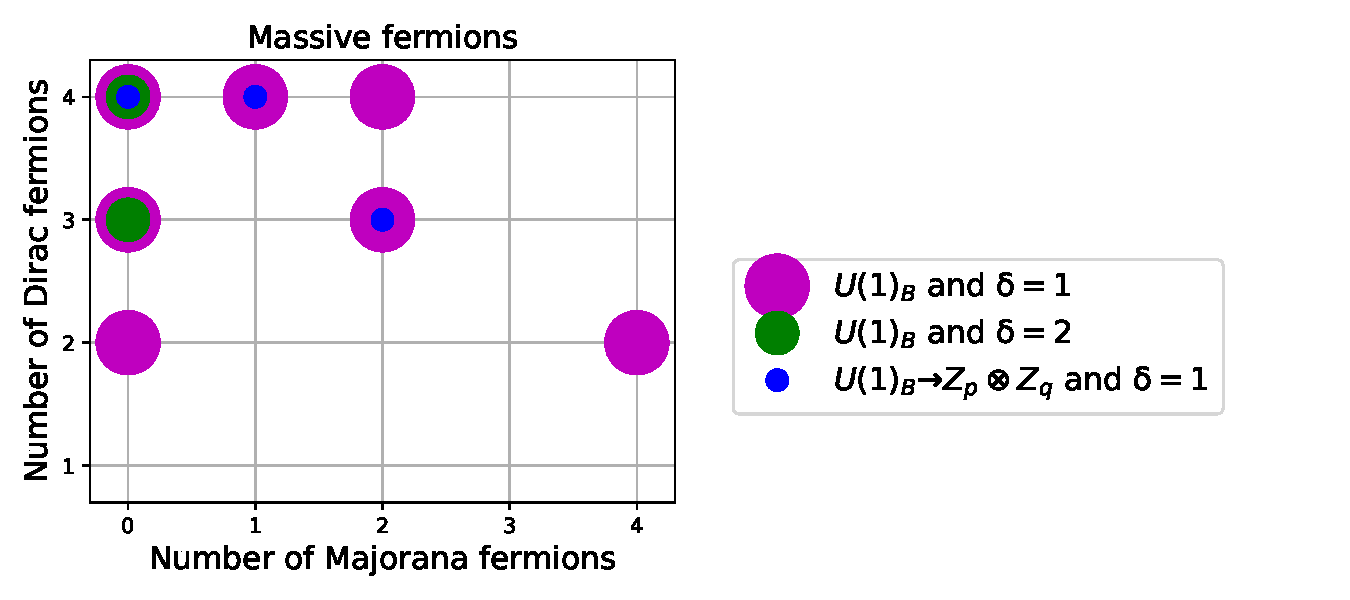
\includegraphics[scale=0.7]{number}
     \caption{Number of massive Dirac and Majorana fermions in each type of the 48 types of solutions of the full set of solutions in Fig.~\ref{fig:solutions}. The discs magenta and cyan (yellow and green) are for dark (active) symmetries which allows the effective Dirac neutrino mass operator for at leas two right-handed neutrinos for D-$4+\delta$, with $\delta=1,2$ respectively. Similarly, the blue and red  points are the type of solutions which satisfy the unconditional stability conditions for at least two DM candidates. }
    \label{fig:number}
\end{figure}
\end{frame}

\begin{frame}
  \frametitle{Multi-component dark matter II}
\begin{figure}
    \centering
    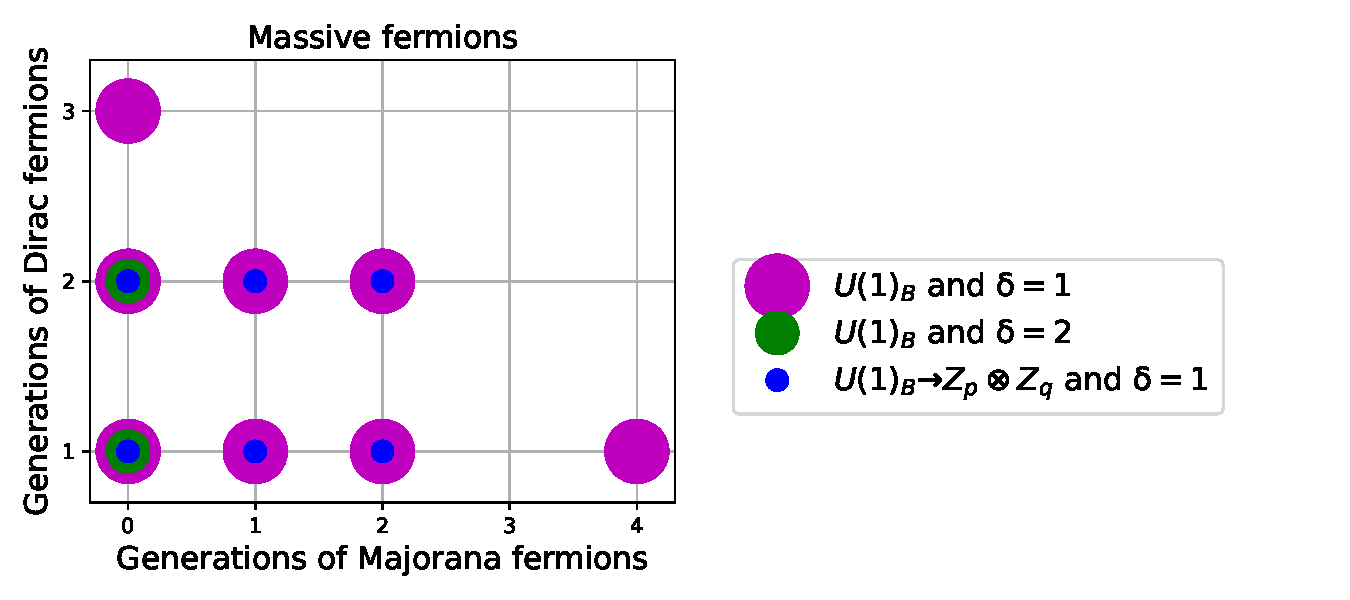
\includegraphics[scale=0.7]{generation}
    \caption{Same as Fig.~\ref{fig:number} 
    but for number generations of massive Dirac and Majorana fermions in each type of the 48 types of solutions of the full set of solutions in Fig.~\ref{fig:solutions}. 
    }
    \label{fig:generation}
\end{figure}  
\end{frame}





\begin{frame}
  \frametitle{Solution: $(3, 3, 3, -5, -5, -7, 8)$}
\begin{table}
  \centering
  \begin{tabular}{l|c|c|c|c                                  }\hline
    Field            &$SU(2)_L$     & $\operatorname{U}(1)_Y$ &$\operatorname{U}(1)_X$ &$ \operatorname{U}(1)_{B-L}$ \\ \hline
    $Q_i$            & $\mathbf{2}$ & $1/6$   & $L/3$ & $1/3$     \\
    $u_{Ri}$         & $\mathbf{1}$ & $2/3$   & $4L/3-3$ & $1/3$     \\
$d_{Ri}$         & $\mathbf{1}$ & $-1/3$   & $3-2L/3$ & $1/3$     \\    
    $L_i$            & $\mathbf{2}$ & $-1/2$   & $-L$ & $-1$     \\ %-3/3
    $e_{Ri}$         & $\mathbf{1}$ & $-1$   & $3-2L$ & $-1$     \\ %-3/3
    $\nu_{R \alpha}$ & $\mathbf{1}$ & $0$      & $-5$ & $-5/3$     \\ %-5/3
    $\psi_1$         & $\mathbf{1}$ & $0$      & $-7 $ & $-7/3 $  \\ 
    $\psi_2$         & $\mathbf{1}$ & $0$      & $8$ & $8/3$    \\
    $H$              & $\mathbf{2}$ & $1/2$    &  $L-3 $ &$0$  \\        
    $S$              & $\mathbf{1}$ & $0$      &  $1$ & $1/3$   \\\hline 
    $\sigma_1^-$     & $\mathbf{1}$ & $-1$    &  $2L $ & $2$  \\ %6/3       
    $\sigma_2^-$     & $\mathbf{1}$ & $-1$    &  $(-2-2L) $ & $-8/3$  \\\hline   %2L+2-2L=2     
  \end{tabular}
  \caption{$X$ and proper $B-L$ normalized charges for the first solution in Table~\ref{tab:sltns}, $(3\c 3\c 3\c -5\c -5\c -7\c 8)$, for which $m=3$, $\nu=-5$, $\delta=2$ and therefore from eq. \eqref{eq:effcon}, $s=1$. For the column $\operatorname{U}(1)_{B-L}$ we fix $L=3$ and change $X\to X/3$. Moreover, $i=1,2,3$ and $\alpha=1,2$. The electroweak quantum numbers are also shown for each one of SM fields, the extra singlet chiral fermions, and the scalars in the last four rows.}
  \label{tab:pickedsltn}
\end{table}




\end{frame}

\begin{frame}
  \frametitle{Neutrino phenomenology}
  with J. Calle and O. Zapata: arXiv:2103.15328  [PRD]

  \begin{figure}
    \centering
    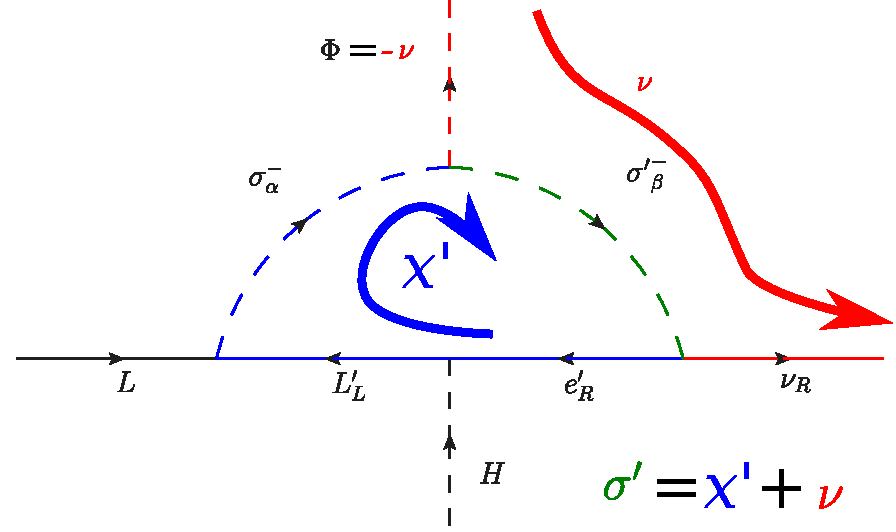
\includegraphics[scale=0.5]{zee2}
    \caption{}
    \label{fig:zee}
\end{figure}
Large GNI, CLFV and LHC dileptons signals
\end{frame}

\begin{frame}
  \frametitle{Dark matter phenomenology}
Michael Duerr, Pavel Fileviez Perez,...  arXiv:1506.05107, arXiv:1409.8165
  
with J. Calle and O. Zapata: arXiv:1909.09574  [PRD]

\begin{figure}
    \centering
    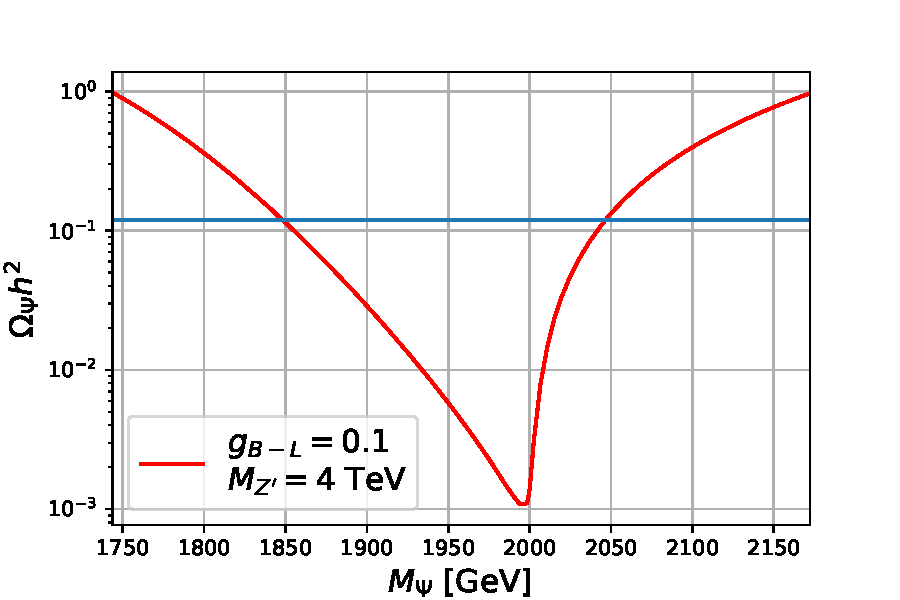
\includegraphics[scale=0.6]{dmz}
    \caption{}
    \label{fig:dm}
\end{figure}

\end{frame}

\begin{frame}
  \frametitle{$\Delta N_{\text{eff}}$}
  \only<1>{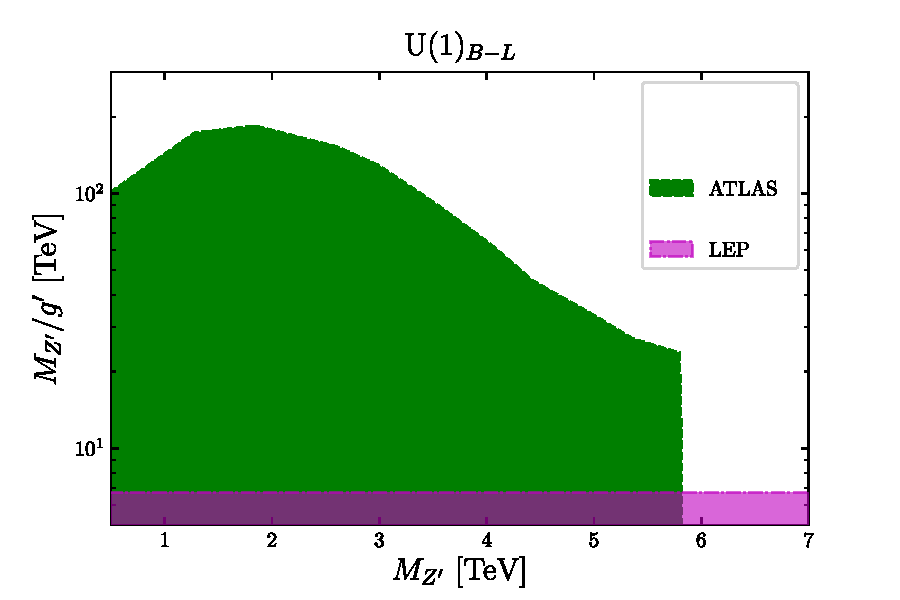
\includegraphics[height=8cm]{u1blc1}}%
  \only<2>{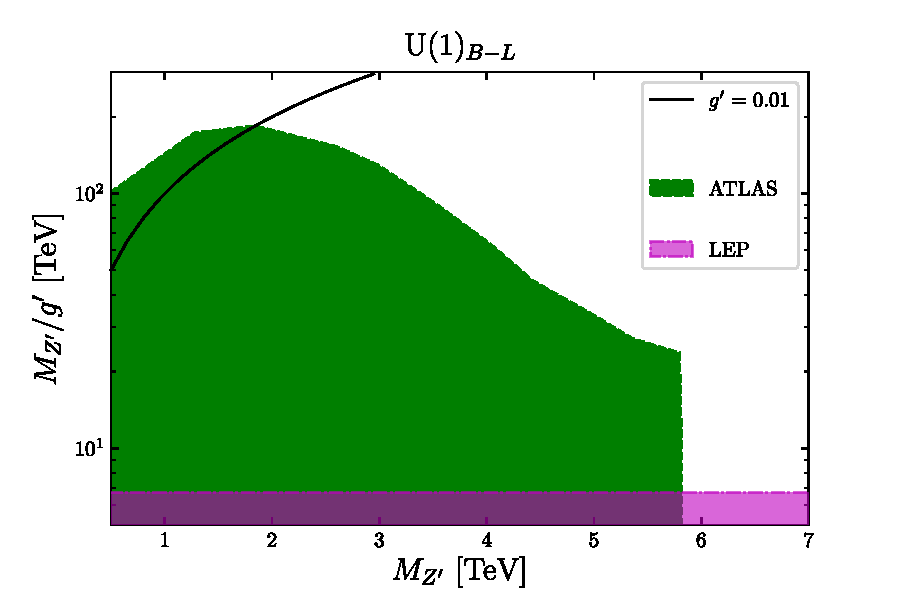
\includegraphics[height=8cm]{u1blc2}}%
  \only<3>{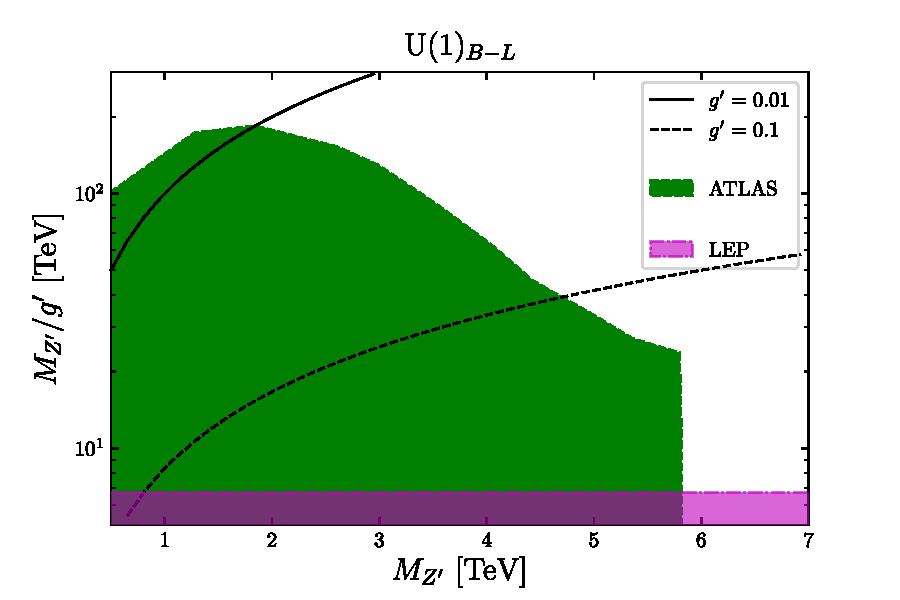
\includegraphics[height=8cm]{u1blc3}}%
  \only<4>{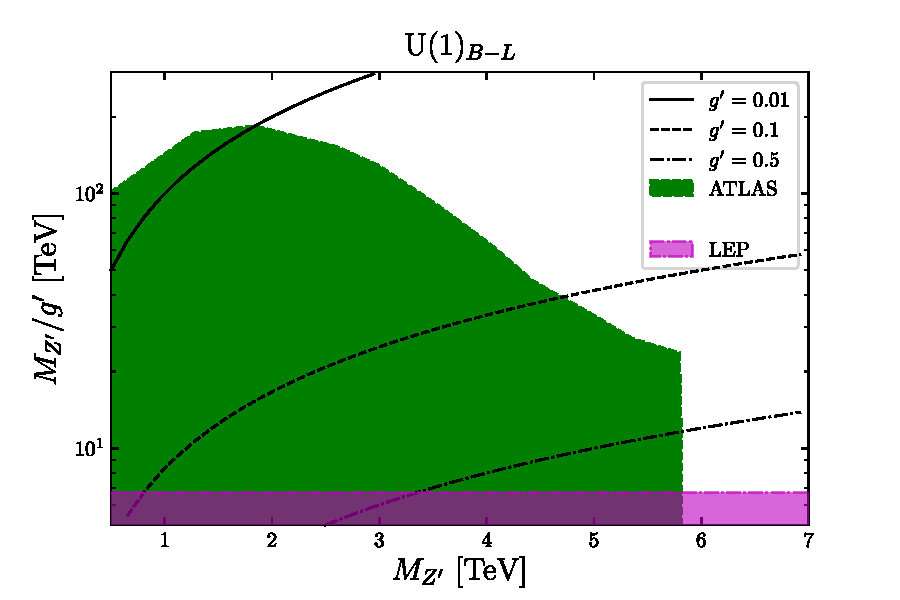
\includegraphics[height=8cm]{u1blc4}}%
  \only<5->{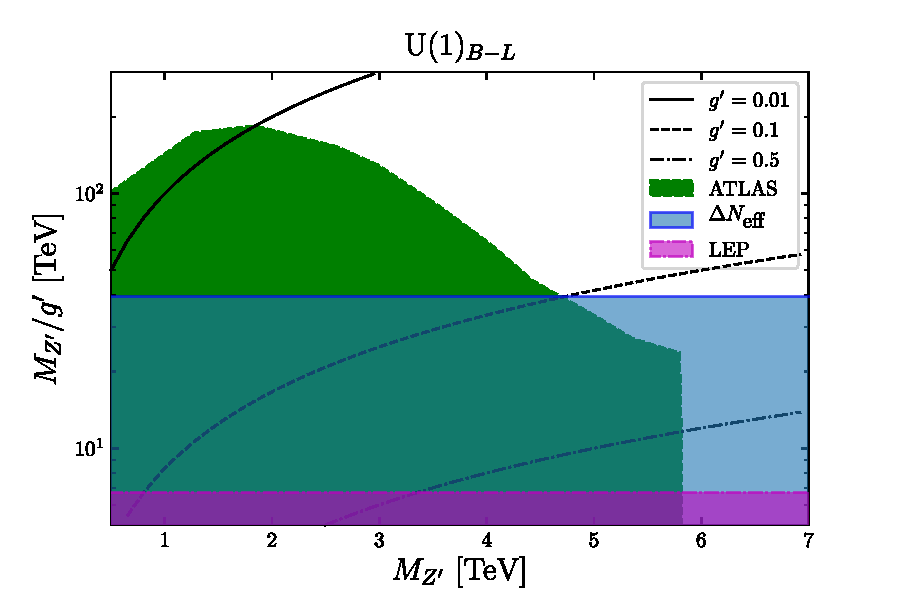
\includegraphics[height=8cm]{u1blc5}}%  
\end{frame}


\begin{frame}
  \frametitle{Dark matter phenomenology}
\begin{figure}
    \centering
    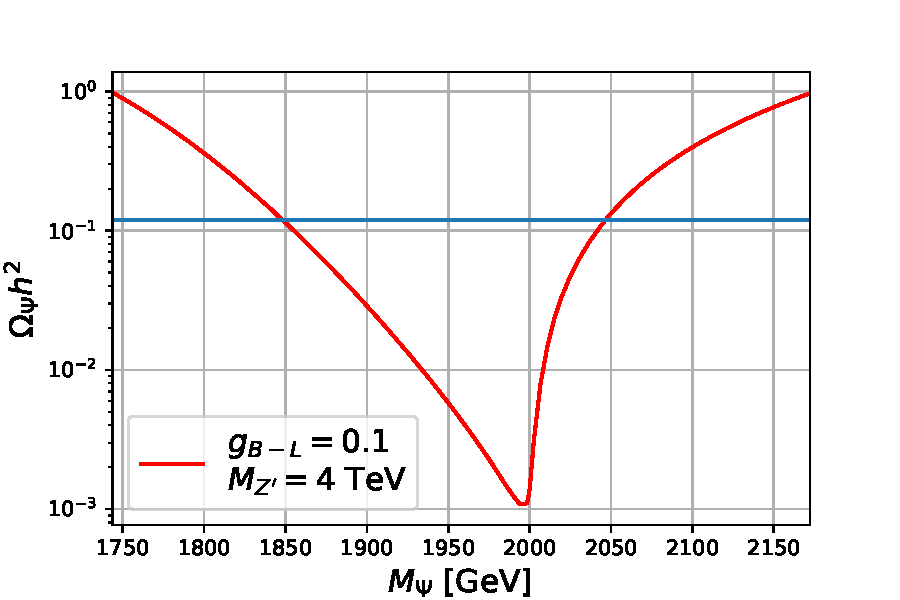
\includegraphics[scale=0.6]{dmz}
    \caption{}
    \label{fig:dm}
\end{figure}

\end{frame}


\begin{frame}
  \frametitle{Conclusions}
  \begin{itemize}
  \item One thousand solutions
  \item 48 types of solutions: $N$, $N_{\text{chiral}}$, $\delta$, $N_D$, $N_M$, $G_D$, $G_M$
  \item The scalar realizations of the effective Dirac neutrino mass operator feature a set of parameters which explain independently the neutrino oscillations and the phenomenology of a multi-component and multi-generational dark matter sector. Large GNI, CLFV, LHC dileptons
  \end{itemize}
  
  In general, we can see that multi-component and multi-generation DM candidates are the trend for gauge Abelian extensions of the SM with massive singlet chiral fermions compatible with the effective Dirac neutrino mass operator of dimension
\end{frame}



\begin{frame}
  \frametitle{One parameter $\operatorname{U}(1)_X$ SM extension }
        \rowcolors{1}{RoyalBlue!20}{}
  \begin{tabular}{c|c|c|c|c|c|c|c||c}
    \hline  
    Fields     & $\operatorname{SU}(2)_L$ & $\operatorname{U}(1)_Y $ & $\operatorname{U}(1)_{X}$& $\color{red}\operatorname{U}(1)_{B-L}$& $\operatorname{U}(1)_R$& $\operatorname{U}(1)_D$& $\operatorname{U}(1)_G$ & $\operatorname{U}(1)_{\mathcal{D}}^{{\color{Yellow}*}}$\\ \hline
$L $  & $\boldsymbol{2}$& $-1/2$  &  ${\color{blue}l}      $&  $\color{red}-1$&    $0$ &  $-3/2$     &  $-1/2$&$0$ \\    
$Q $  & $\boldsymbol{2}$& $-1/6$  &  $-{\color{blue}l}/3   $& $\color{red}1/3$&    $0$&  $1/2$    &  $1/6 $&$0$ \\
$d_R $& $\boldsymbol{1}$& $-1/2$  &  $1+2{\color{blue}l}/3 $&  $\color{red}1/3$&    $1$&  $0$ &  $2/3 $&$0$ \\
$u_R $& $\boldsymbol{1}$& $+2/3$  &  $-1-4{\color{blue}l}/3$&  $\color{red}1/3$&   $-1$&  $1$&  $-1/3$&$0$ \\
$e_R $& $\boldsymbol{1}$& $-1$    &  $1+2{\color{blue}l}   $&  $\color{red}-1$&    $1$ &  $-2$    &  $0   $&$0$ \\
$H $  & $\boldsymbol{2}$& $1/2$  &   $-1-{\color{blue}l}   $&  $\color{red}0$&    $-1$ &  $1/2$   &  $-1/2$&$0$ \\\hline
%$S$ & $\boldsymbol{1}$ & $0$  & $ 2 \psi_N$& $\color{red}2 \psi_N$&  $2 \psi_N$ & $2 \psi_N$& $2 \psi_N$ &$0$ \\
 $\sum_\alpha n_{\alpha}$ & $\boldsymbol{1}$ & $0$ & $-3$& $\color{red}-3$&  $-3$ & $-3$& $-3$&$0$\\
 $\sum_\alpha n_{\alpha}^{3}$ & $\boldsymbol{1}$ & $0$ & $-3$& $\color{red}-3$&  $-3$ & $-3$& $-3$&$0$\\ \hline
  \end{tabular}

  % {\color{Yellow}*} Use vector like fermions $\mathcal{D}(\psi_L)=\mathcal{D}(\psi_R)\to n-n=0$
  
  % Solutions in terms of a parameter: arXiv:1811.11927, N. Okada, \emph{et al} [PRD];

  % and some specific examples from: arXiv:1705.05388,  Farinaldo Queiroz,  \emph{et al} [JHEP]

  % \alert{All known $\operatorname{U}(1)_{B-L}$ (radiative) neutrino solutions apply for $\operatorname{U}(1)_X$}:
\end{frame}


\begin{frame}
  \frametitle{\invisible<1>{Or$\cdots$ combine known} solutions \only<1>{with $\sum n_{\alpha}=-3$ and $\sum n_{\alpha}^3=-3$}\only<2>{with $\sum n_{\alpha}=0$ and $\sum n_{\alpha}^3=0$}}
  \vspace{-0.7cm}
\begin{columns}
  \begin{column}{0.72\textwidth}
    \begin{table}
  \centering
  \renewcommand{\arraystretch}{1.4}
      \rowcolors{1}{RoyalBlue!20}{}
  \begin{tabular}{c|l}\hline
$\left(\nu_{R1},\nu_{R2},\psi_{N-2},\cdots\right)$     & Ref \\ \hline
    $\left(-1,-1,-1\right)$&\tiny hep-ph/0611205, S. Khalil  [JPG] \\
    $\color{red}\left(-4,-4,+5\right)$&
\includegraphics[scale=0.03]{brazil}\tiny arXiv:0706.0473, Montero, V. Pleitez [PLB]\\
    $\left(-\dfrac{2}{3},-\dfrac{2}{3},-\dfrac{4}{3},-\dfrac{1}{3}\right)$&
\includegraphics[scale=0.03]{colombia}\tiny  arXiv:1607.04029, S. Patra , W. Rodejohann, C. Yaguna [JHEP] \\
    $\color{red}\left(-\dfrac{8}{5},-\dfrac{8}{5},-\dfrac{2}{5},-\dfrac{7}{5},+2\right)$&
\includegraphics[scale=0.03]{colombia}\tiny arXiv:1812.05523, with J. Calle, C. Yaguna, Ó. Zapata [PRD]\\
    %$\left(-\dfrac{7}{3},-\dfrac{7}{3},+\dfrac{1}{3},-\dfrac{5}{3},+3\right)$&\cite{}\\
    %$\left(-\dfrac{7}{10},-\dfrac{7}{10},-\dfrac{13}{10},-\dfrac{1}{2},+\dfrac{1}{5}\right)$&\cite{}\\
    $\left( -1,-1,-\dfrac{10}{7},-\dfrac{4}{7},-\dfrac{2}{7},\dfrac{9}{7} \right)$ &
\includegraphics[scale=0.03]{colombia} \tiny 1808.03352, with N. Bernal, C. Yaguna, Ó. Zapata [PRD]\\
    $\left( -\dfrac{5}{3},-\dfrac{5}{3},-\dfrac{7}{3},\dfrac{8}{3} \right)$ &
\includegraphics[scale=0.03]{brazil}
\includegraphics[scale=0.03]{colombia}\small In progress...  
\includegraphics[scale=0.08]{new} method$ {}^{\color{blue}\dagger}$ \\
    \hline
   \end{tabular}
   \caption{\scriptsize Possible solutions with at least two repeated charges and until six chiral fermions.

   ${}^{\color{blue}\dagger}$ General $\sum n_\alpha=0$ solutions: see {\tiny D.B Costa, \emph{et al}, \arXiv{1905.13729} [PRL]}}
      \label{tab:sltn5}
\end{table}


\end{column}
\begin{column}{0.28\textwidth}
    \begin{picture}(100,200)
  \only<2>{\put(-85,100){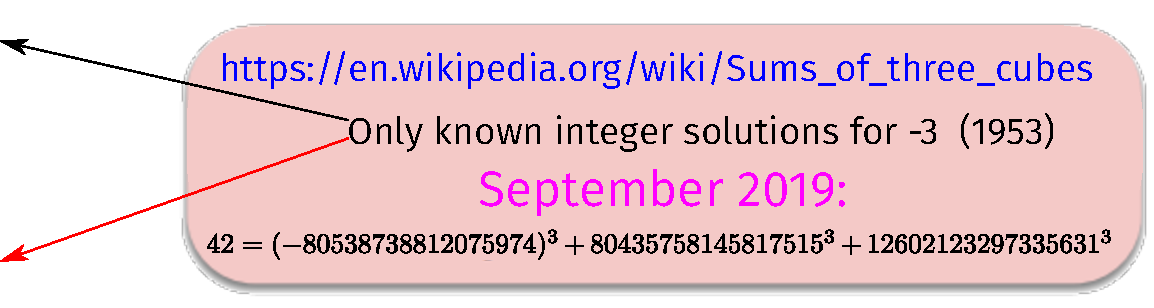
\includegraphics[scale=0.41]{nomajo1}}}%
  \only<3>{\put(-85,100){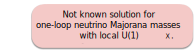
\includegraphics[scale=0.41]{nomajo} }}%
    \end{picture}

    \vspace{-2cm}

        \invisible<1-2>{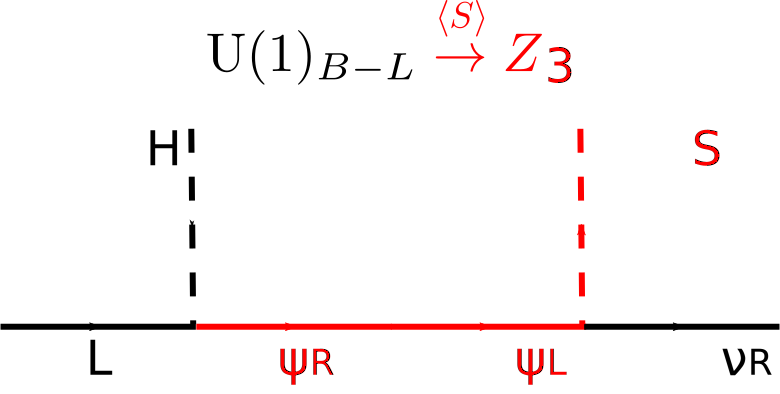
\includegraphics[scale=0.14]{tree-level-dirac-seesaw}

      {\scriptsize
          \rowcolors{1}{RoyalBlue!20}{}
  \begin{tabular}{cccccc}\hline
   $ \nu_{R3} $
  &$\nu_{R2} $&$\nu_{R1}$&$\psi_L$&$ \psi_R  $&$S$\\ \hline
  $\color{red}-4$&$\color{red}-4$&$\color{red}+5$& $\color{black}-1$ & $\color{black}-1$ & $+3$\\\hline
  \end{tabular}

  {\tiny E. Ma, R. Srivastava: arXiv:1411.5042 [PLB]}
}}
\end{column}
\end{columns}

\end{frame}


\begin{frame}
\begin{picture}(320,250)
\only<1->{\put(-24,-22){\begin{overpic}[scale=0.352]{z2_bkg}\end{overpic}}}%
%\only<1>{\put(194,92){\begin{overpic}[scale=0.2]{infinity}\end{overpic}}}%
\only<1->{\put(30,160.5){ $\invisible<1-3>{\langle}\mathbf{SM}\invisible<1-3>{\rangle}$  }}%
\only<1->{\put(18,115){\begin{overpic}[scale=0.1]{smfp}\end{overpic}}}%
\only<1->{\put(38,105){ {\large +}  }}%
\only<1->{\put(0,100){\Large  $m^{\nu}_{\text{Majorana}}=\dfrac{h_{\nu}}{\Lambda} L \cdot H L \cdot H\invisible<1-3>{\dfrac{\color{red}S}{\Lambda}}$ \invisible<1,3->{\color{red}(three-level)}   }}%
\only<2->{\put(-32,80){ {\scriptsize Type-I arXiv:1808.03352\only<2>{, II arXiv:1607.04029, III arXiv:1908.04308}\only<3>{, with N. Bernal, C. Yaguna, and Ó. Zapata [PRD]}\only<4->{
        \begin{minipage}[t]{2.7cm}
          \color{red}: Also new terms arise from spontaneous breakdown of a new gauge symmetry
        \end{minipage}
} } }}%
\only<2-3>{\put(204,158){ \begin{overpic}[scale=0.27]{alert}\end{overpic}}}%
\only<2-3>{\put(224,195){ {\huge \only<1-2>{\textbf{3 models}}\only<3->{
        \hspace{0.4cm}\begin{minipage}{3cm}
          Type-I\\
          seesaw
        \end{minipage}
      }}  }}%
\only<3->{\put(-10,200){\Large $\mathcal{L}=y\left( N_R \right)^{\dagger}L \cdot \invisible<1-3>{\langle}H\invisible<1-3>{\rangle}+  \only<3>{M_N}\only<4->{y'{\color{red} \langle S\rangle}}  N_R N_R+\text{h.c} $   }}%
\only<4->{\put(124,218.5){ \Huge \invisible<4>{{\color{red}Lo}{\color{Yellow}cal}} $U(1)_{B-L} \color{red} \to  Z_7 $  }}%
\only<4->{ \put(153,155){
    %\scriptsize
          \rowcolors{1}{RoyalBlue!20}{}
    \begin{tabular}{cccccccc}\hline
   $ \nu_{R3} $
      &$\nu_{R2} $&\invisible<1-4>{$\color{red}\overline{\psi_{L1}}$}&\invisible<1-4>{$\color{red}\psi_{R1}$}&\invisible<1-4>{$\color{Yellow} \psi_{R2}  $}&\invisible<1-4>{$\color{Yellow}\overline{\psi_{L2}}}$ &{ $S$} & \invisible<1-4>{$\color{Yellow}S'$}\\ \hline
  $-1$&$-1$&\invisible<1-4>{$\color{red}-\dfrac{10}{7}$}&\invisible<1-4>{ $\color{red}-\dfrac{4}{7}$} & $\invisible<1-4>{\color{Yellow}-\dfrac{2}{7}$} &\invisible<1-4>{ $\color{Yellow}\dfrac{9}{7}$}&$2$&\invisible<1-4>{$\color{Yellow}1$}\\\hline
  \end{tabular}
}   }
\only<5>{\put(204,-20){ \begin{overpic}[scale=0.2]{tcdm}\end{overpic}}}%
\end{picture}
\end{frame}



\begin{frame}
  \frametitle{\only<1>{One loop topologies $\operatorname{U}(1)_{B-L}\oplus Z_2 \oplus Z_2 $}\only<2-4>{One loop topologies $\operatorname{U}(1)_{B-L}$ only!
   \invisible<2>{\scriptsize with J. Calle, C. Yaguna, and O. Zapata, arXiv:1812.05523 [PRD]  } }\only<5-6>{
    SD${}^{3}$M+SSDM: $\sigma_a$ ($a=1,2$)     \invisible<6>{\scriptsize with J. Calle, C. Yaguna, and O. Zapata, arXiv:1812.05523 [PRD]  }  }}
\begin{picture}(320,250)
  \only<1>{\put(40,20){\begin{overpic}[scale=0.6]{radiativedirac1}\end{overpic}}}%
  \only<1>{\put(280,130){\tiny Chang-Yuan Yao and Gui-Jun Ding, arXiv:1802.05231 [PRD]  }}%
  \only<2>{\put(40,20){\begin{overpic}[scale=0.6]{radiativedirac2}\end{overpic}}}%
  \only<2>{\put(280,130){\tiny with J. Calle, C. Yaguna, and O. Zapata, arXiv:1812.05523 [PRD]  }}%
    \only<2-5>{\put(-20,130){\tiny
        \begin{minipage}{0.3\linewidth}
          \begin{align*}
            \psi_{L,R}\to&\text{Singlet fermions \only<3>{(vector-like)}\only<4-5>{(quiral)}  }\\
            \invisible<3>{\Psi_{L,R}\to&\text{Vector-like doublet fermions}\invisible<2-4>{:\qquad {\color{red}10/5}}   }\\
            \sigma\to&\text{Singlet scalar}\invisible<2-4>{:\qquad 15/5}   \\
            \invisible<5>{\eta\to&\text{Doublet scalar}   }
          \end{align*}
        \end{minipage}
}}%
\only<3>{\put(40,20){\begin{overpic}[scale=0.6]{radiativedirac3}\end{overpic}}}%
% 
\only<3>{\put(160,230){\tiny $\longmapsto$ ${\color{Green}\sigma_1}={\color{red}-2}$\,,\qquad
                             ${\color{red}\sigma_2}={\color{Yellow}-5}$\,,\qquad }}%
\only<3>{\put(160,220){\tiny $\longmapsto$ generalization to two and three loops: S. Saad arXiv:1902.07259 [NPB]  }}%
\only<3>{\put(160,210){\tiny $\longmapsto$ generalization to $\operatorname{U(1)_R}$: \emph{et al}, S. Saad arXiv:1904.07407  }}%
\only<3>{\put(180,180){\Huge $\uparrow$   }}%
\only<3-5>{\put(240,135){\tiny
    \begin{minipage}{0.3\linewidth}
      \rowcolors{1}{RoyalBlue!20}{}
  \begin{tabular}{c|cccccc}\hline
 Fields: $f_i$  &  $\left( \nu_{R3} \right)^{\dagger}$
  &$\left( \nu_{R2} \right)^{\dagger}$&$\left( \nu_{R1} \right)^{\dagger}$&$\psi_L$&$\left( \psi_R \right)^{\dagger}$&$S$\\ \hline
  (A)&$\color{Yellow}+4$&$\color{Yellow}+4$&$-5$& $\color{red}-r$ & $\color{red}r$ & $+3$\\
    \invisible<3>{(B) &$\displaystyle{+\frac{8}{5}}$&$\displaystyle{+\frac{8}{5}}$&$\displaystyle{+\frac{2}{5}}$&$\displaystyle{\frac{7}{5}}$&$\color{red}\displaystyle{-\frac{10}{5}}$&$\color{blue}\displaystyle{+\frac{3}{5}}$}\\
  \end{tabular}
         \end{minipage}
       }}%
\only<3-5>{\put(300,55){\tiny
    \begin{minipage}{0.3\linewidth}
       \begin{center}
         \textbf{Anomaly cancellation conditions}
         \begin{align*}
           \sum_i f_i=& 3 \\
           \sum_i f_i^3=& 3 \\
         \end{align*}
  \end{center}
      
         \end{minipage}
       }}%
%  effective number of relativistic degrees of reedom Neff for neutrinos
 \only<4>{\put(40,20){\begin{overpic}[scale=0.6]{radiativedirac4}\end{overpic}}}%
 \only<5-6>{\put(40,20){\begin{overpic}[scale=0.6]{radiativedirac5}\end{overpic}}}%
 \only<6>{\put(20,200){
     \begin{minipage}{0.3\linewidth}
       $M_\psi=h_1 \left\langle S \right\rangle$, $\color{red}y_2=0$:
          \begin{align*}
            \mathcal{L}={\color{red}\mathcal{L}_{\text{SD${}^3$M}}}
            +{\color{Green} h_3^{ia} \widetilde{\left( \Psi_R \right)}\cdot L_i\, \sigma_a}+
      {\color{blue}      h_2^{\beta a} \left( \nu_{R\beta} \right)^{\dagger} \psi_L\, \sigma^{*}_a}
            -V(\sigma_a,S,H)\,.
          \end{align*}
        \end{minipage}
}}%
\only<6>{\put(0,130){\small with A.F Rivera, W. Tangarife,  arXiv:1906.09685 [PRD]   }}%
\only<6>{\put(220,60){\begin{overpic}[scale=0.6]{sarah}\end{overpic}}}%
\end{picture}
\end{frame}





\begin{frame}
  \frametitle{\invisible<1>{Dirac }Radiative Type-I seesaw \only<1>{$\to$Local: only $\operatorname{U}(1)_{B-L}$! {\tiny arXiv:1812.05523, with J. Calle, C. Yaguna, Ó. Zapata [PRD]}} \only<2->{{with Majorana mediators }{\tiny with J. Calle and Ó. Zapata, arXiv:1909.09574}}}
  \begin{columns}
    \begin{column}{0.65\textwidth}
      \def\rssc{0.26}%
      \only<1>{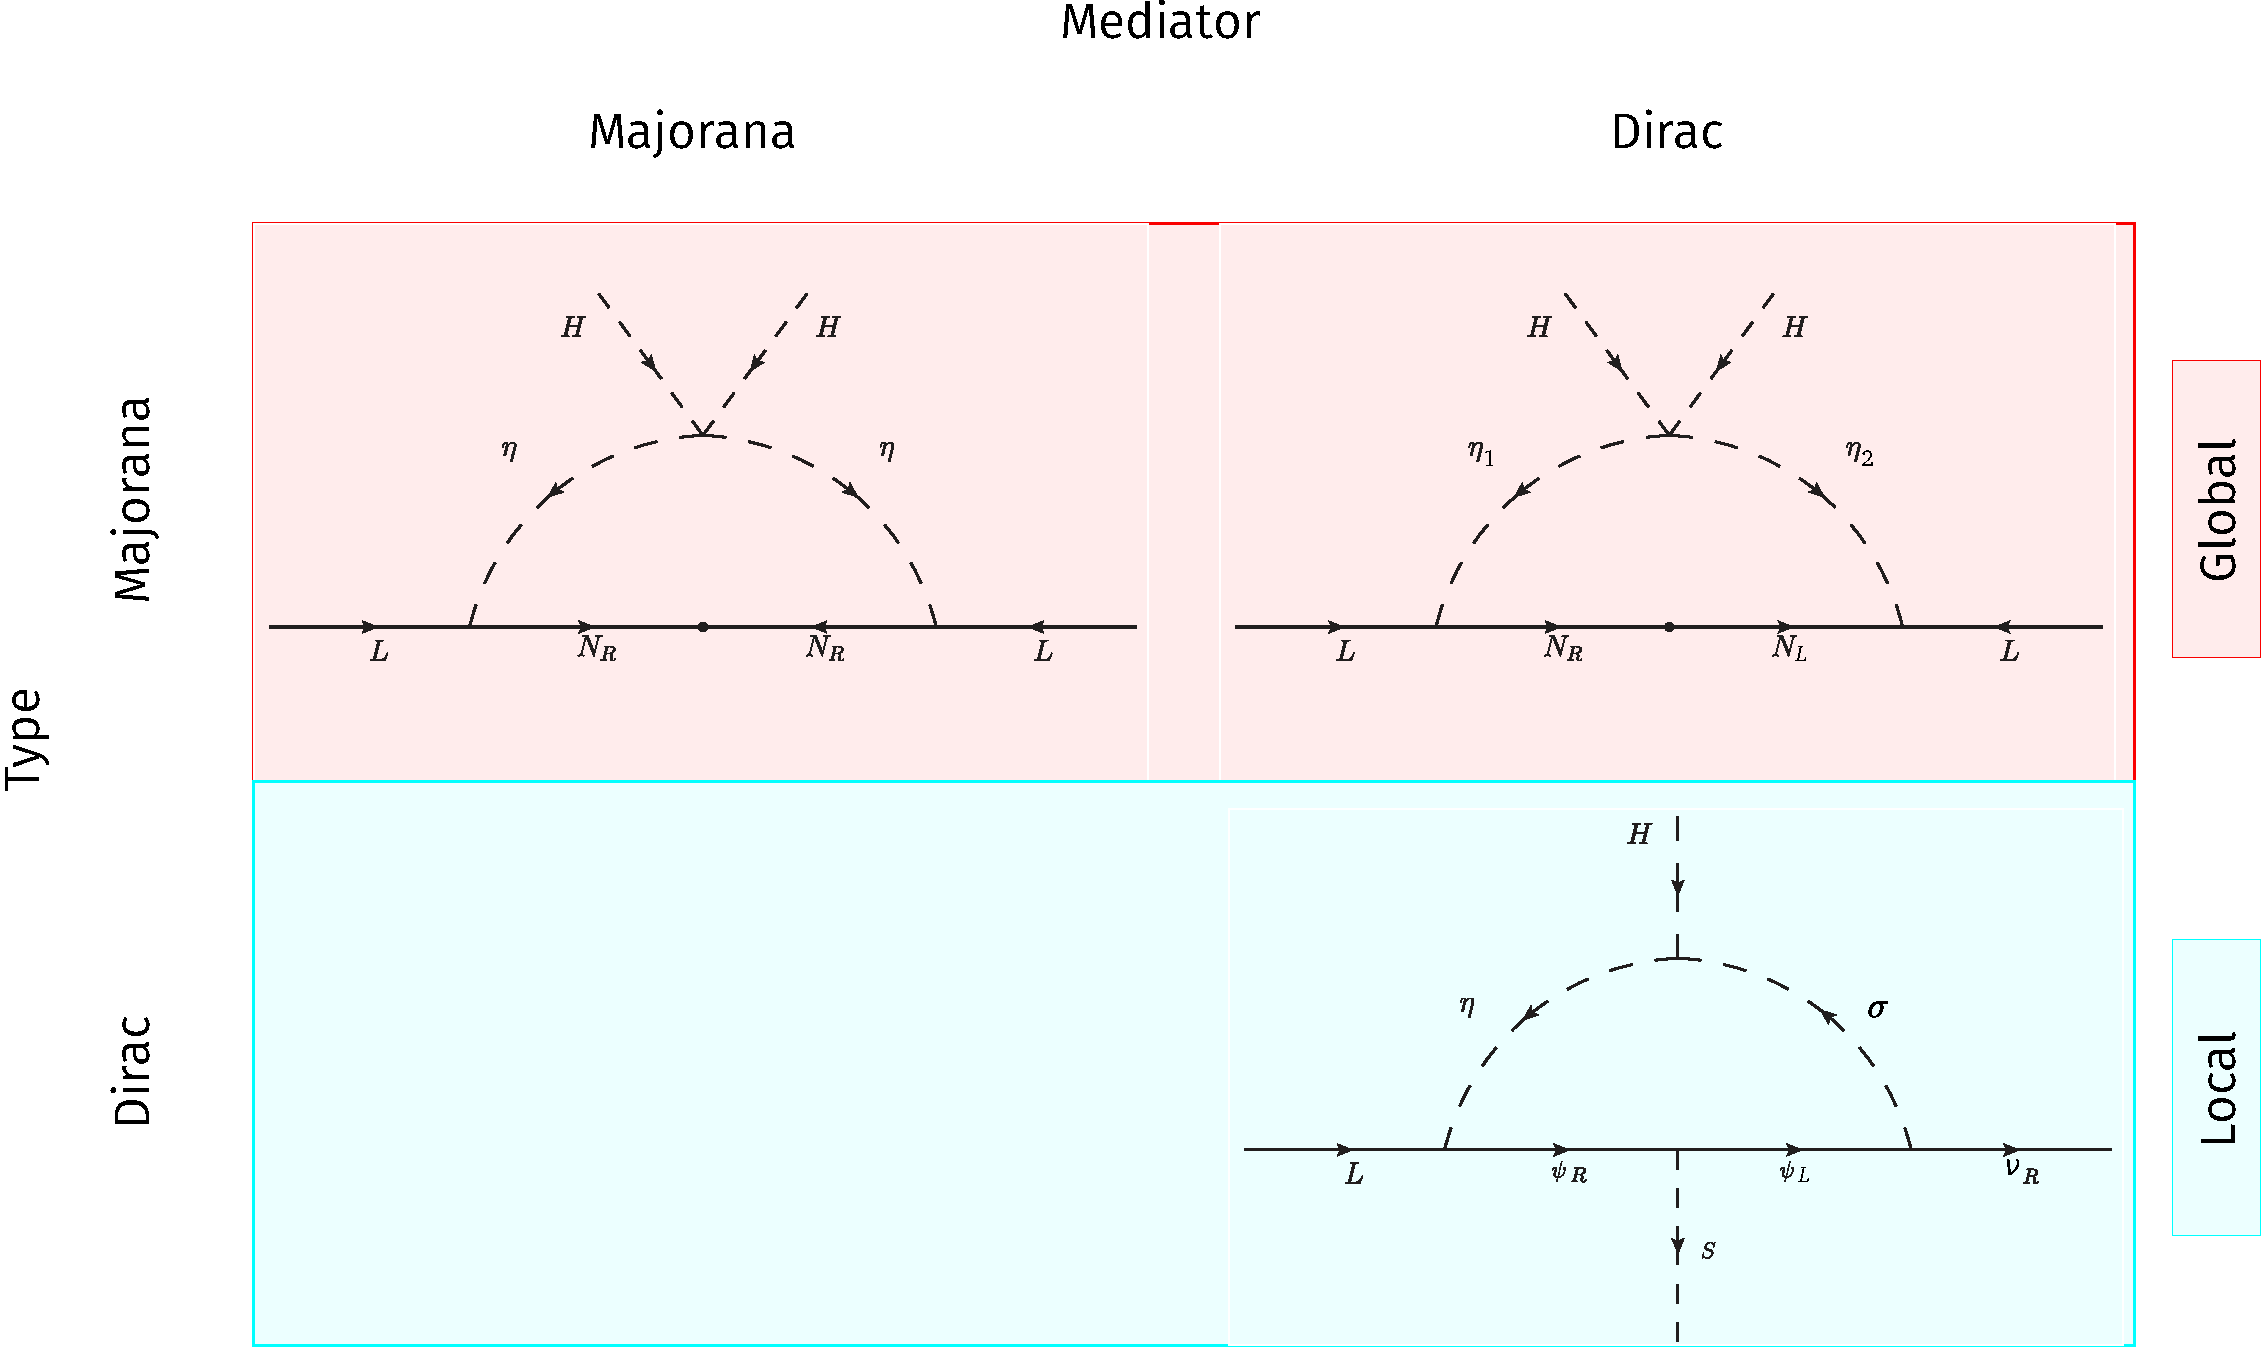
\includegraphics[scale=\rssc]{radiativeseesaw1}}%
      \only<2>{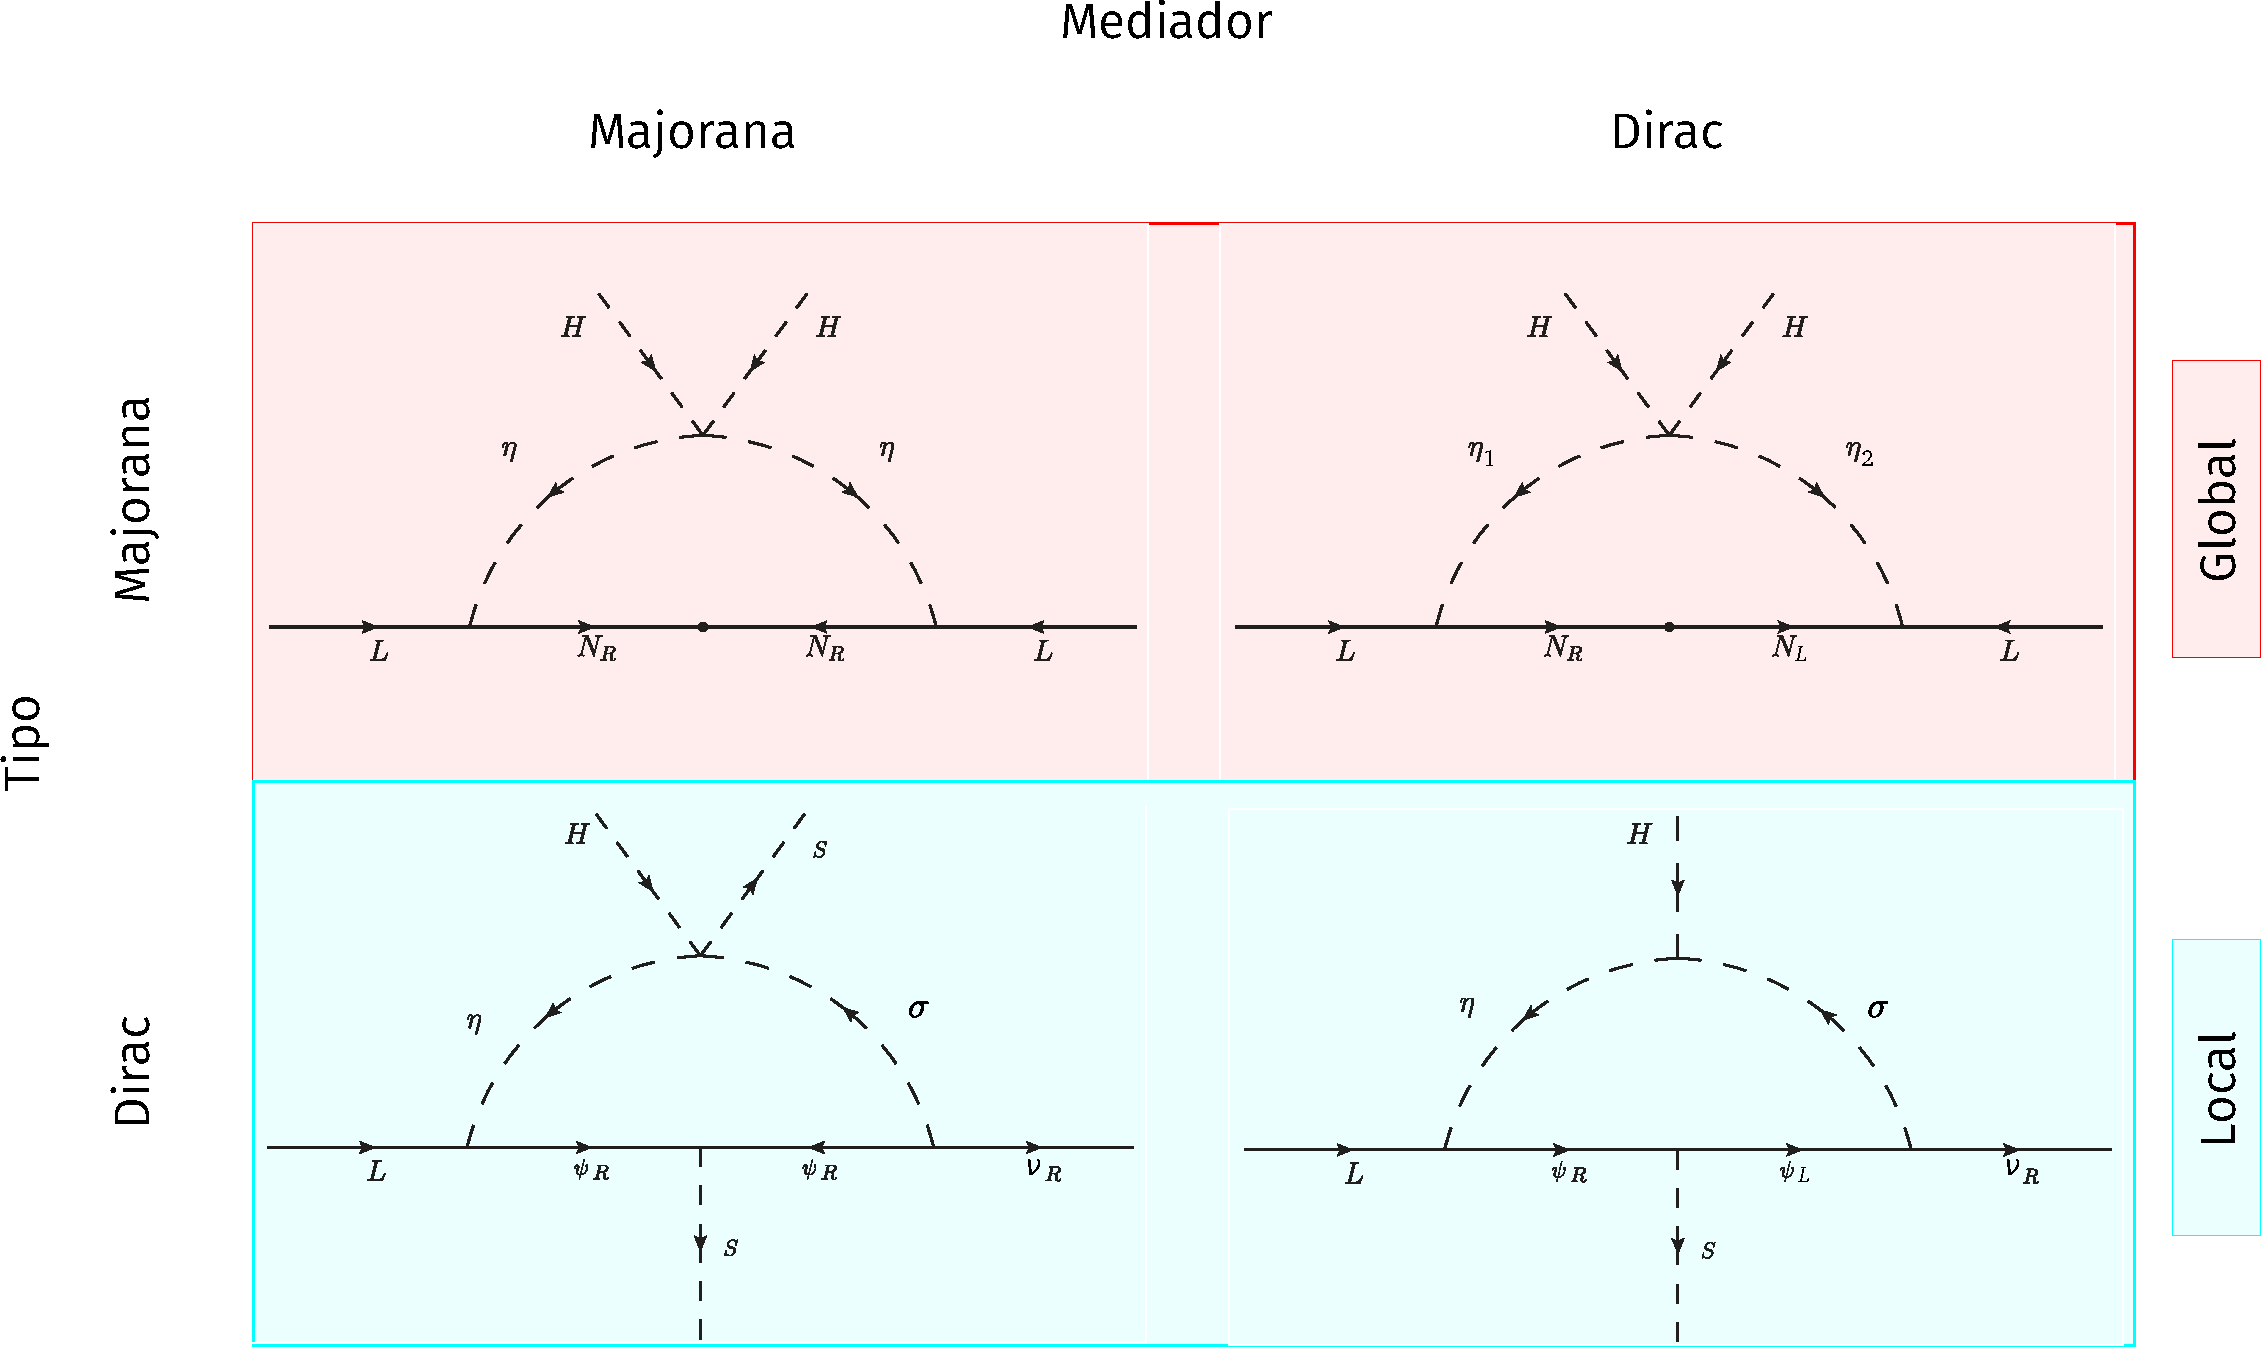
\includegraphics[scale=\rssc]{radiativeseesaw2}}%
      \only<3>{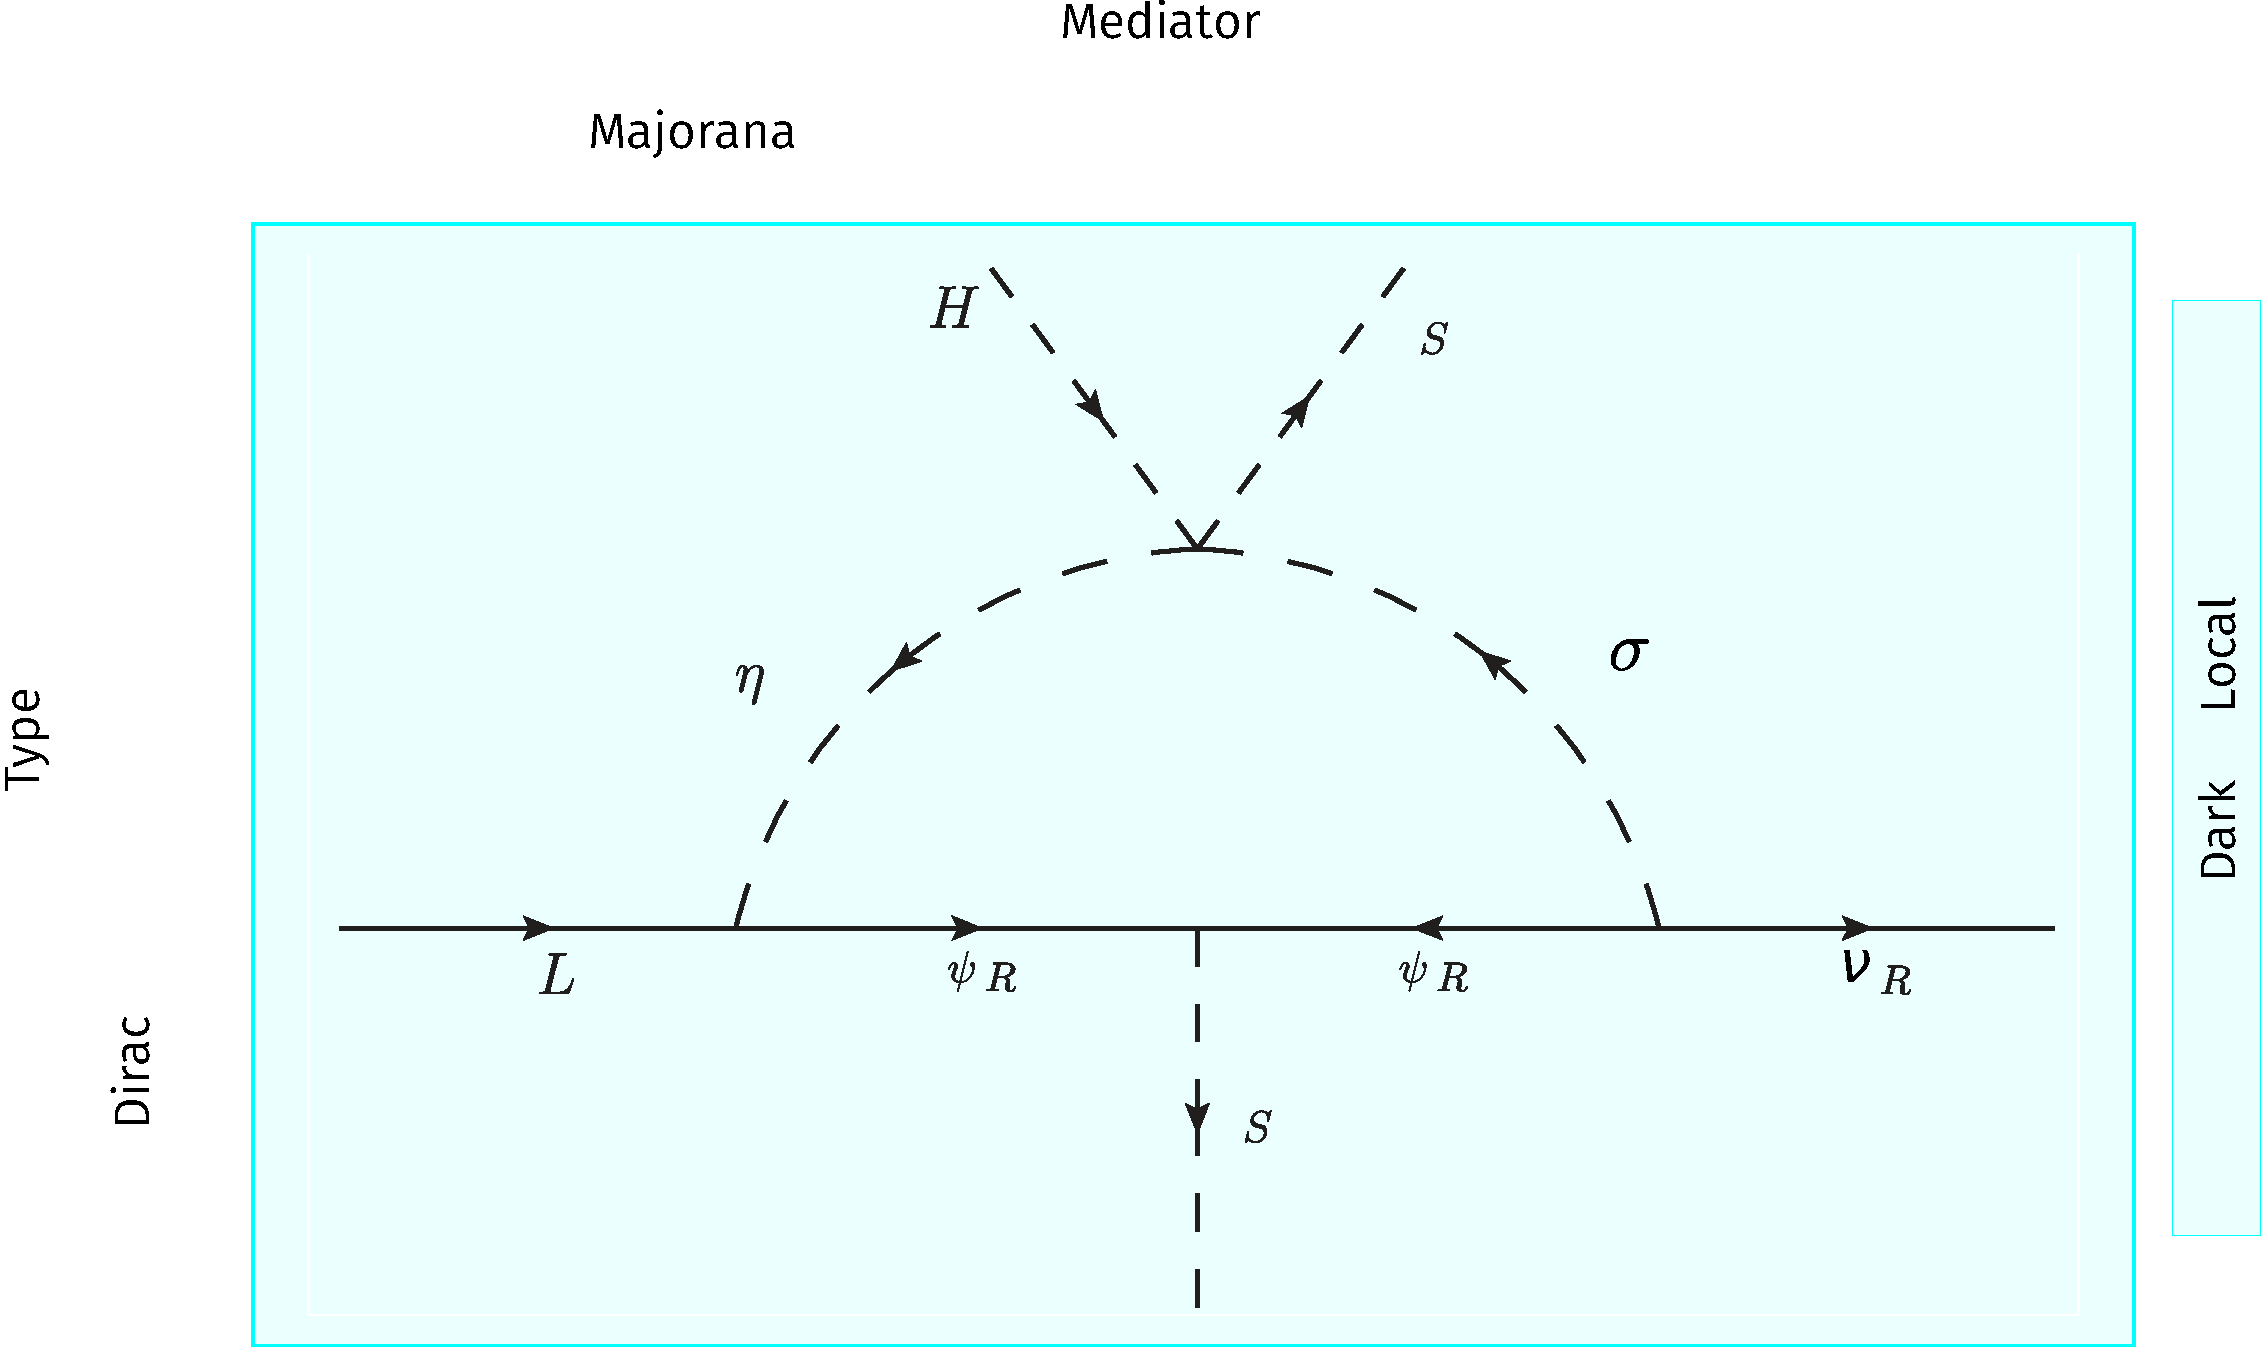
\includegraphics[scale=\rssc]{diracradiativeseesawmajo1}}%
      \only<4>{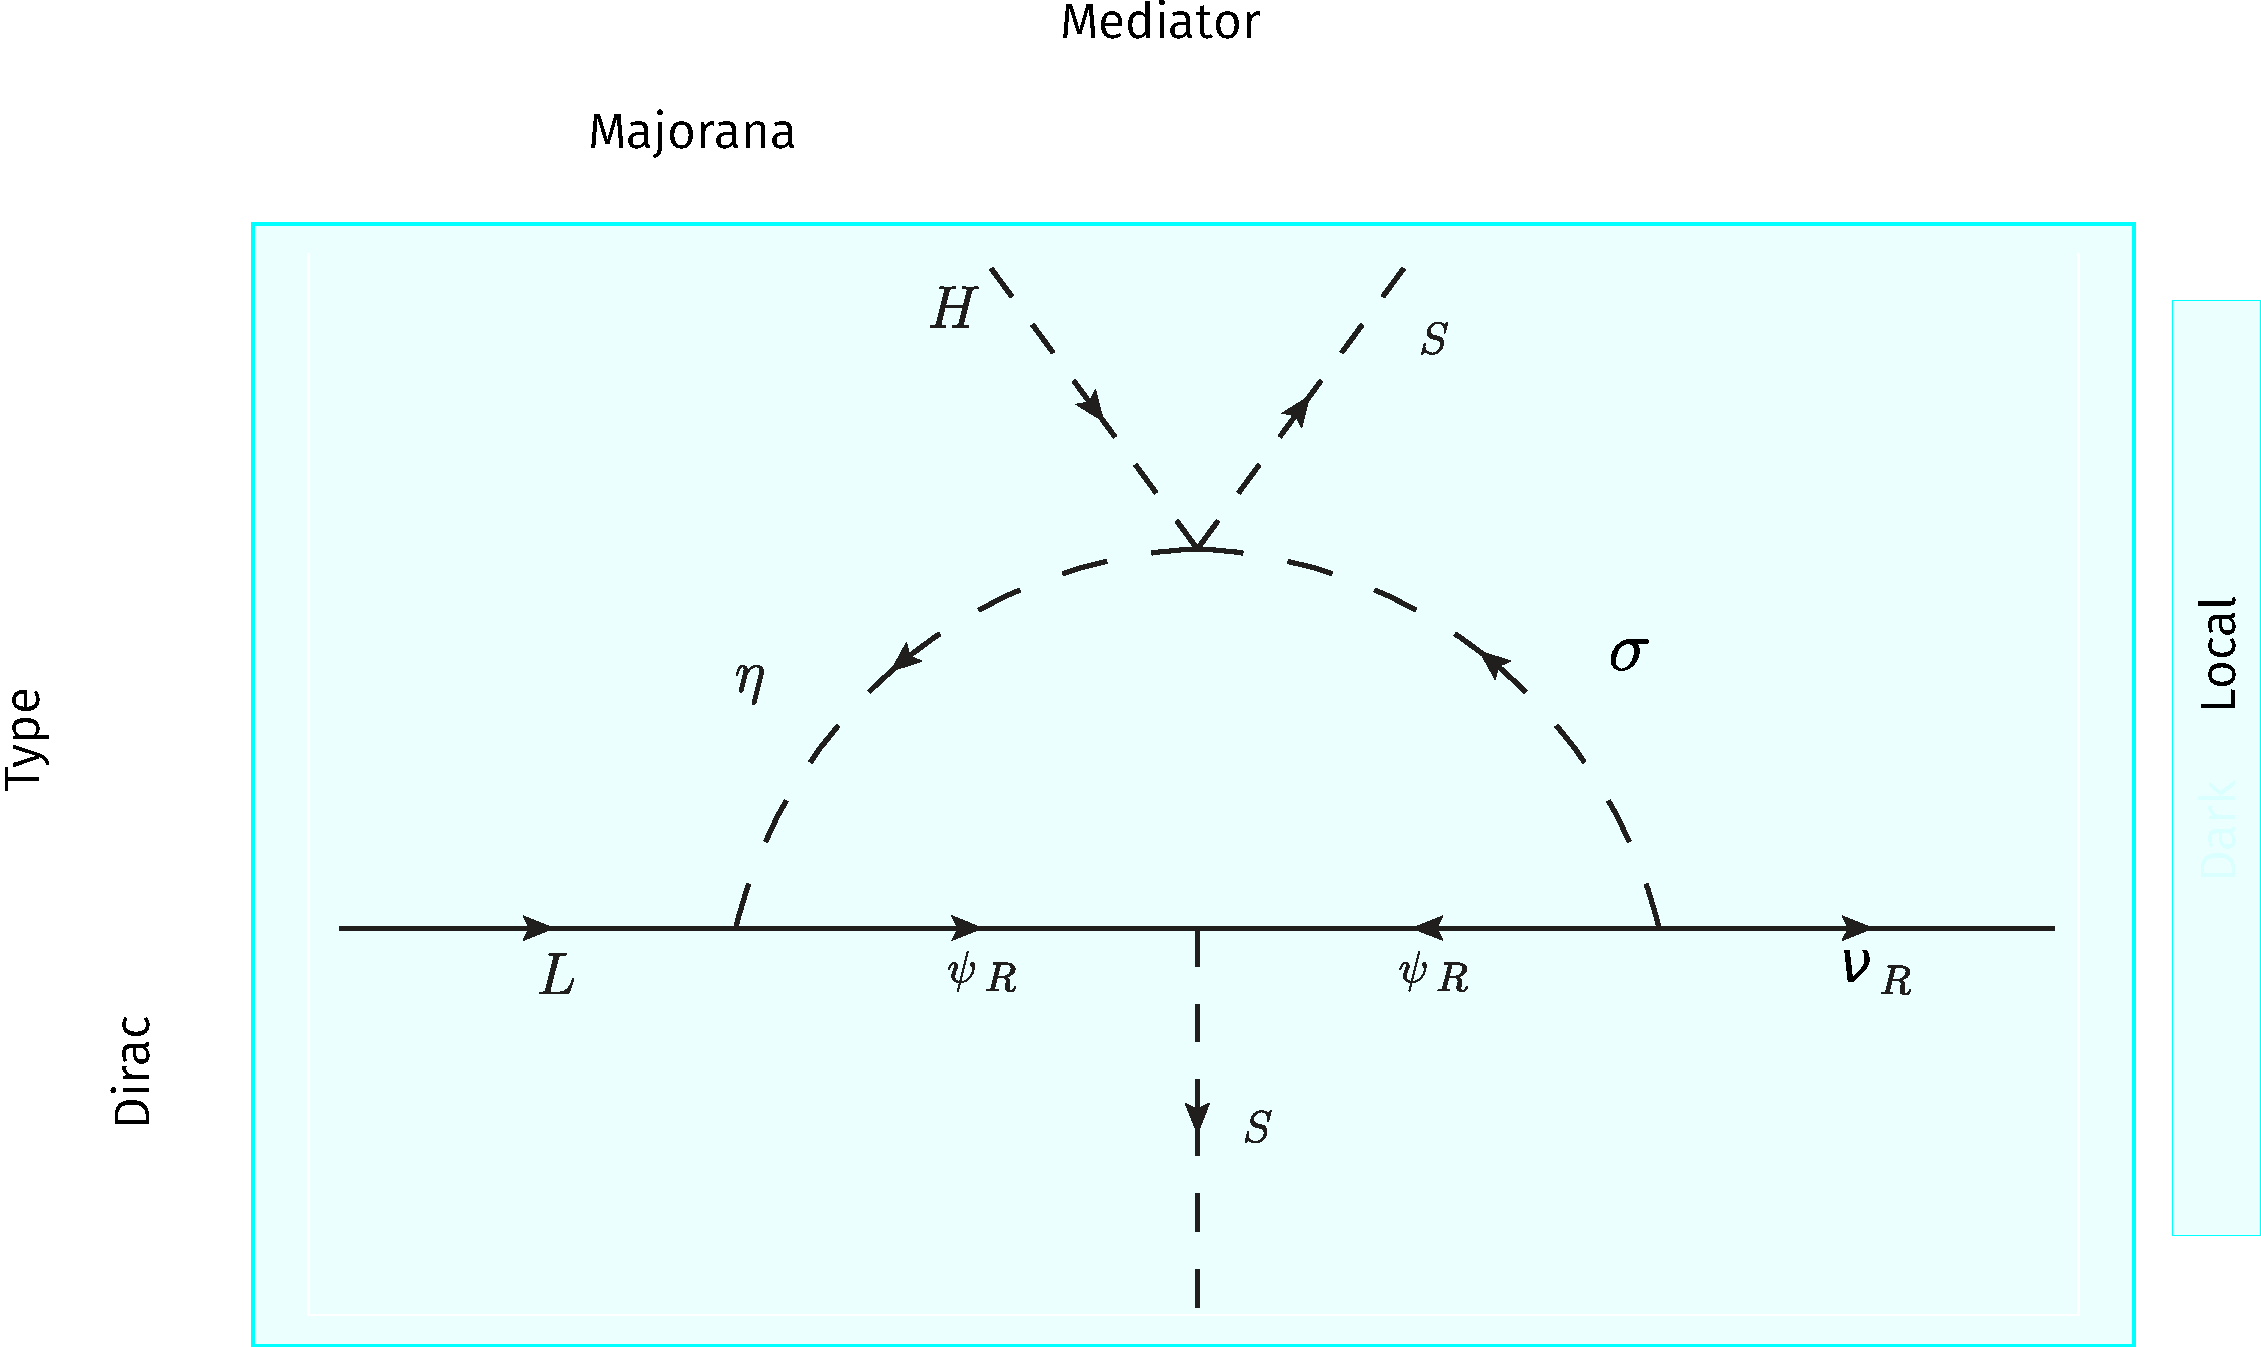
\includegraphics[scale=\rssc]{diracradiativeseesawmajo2}}%
      \only<5>{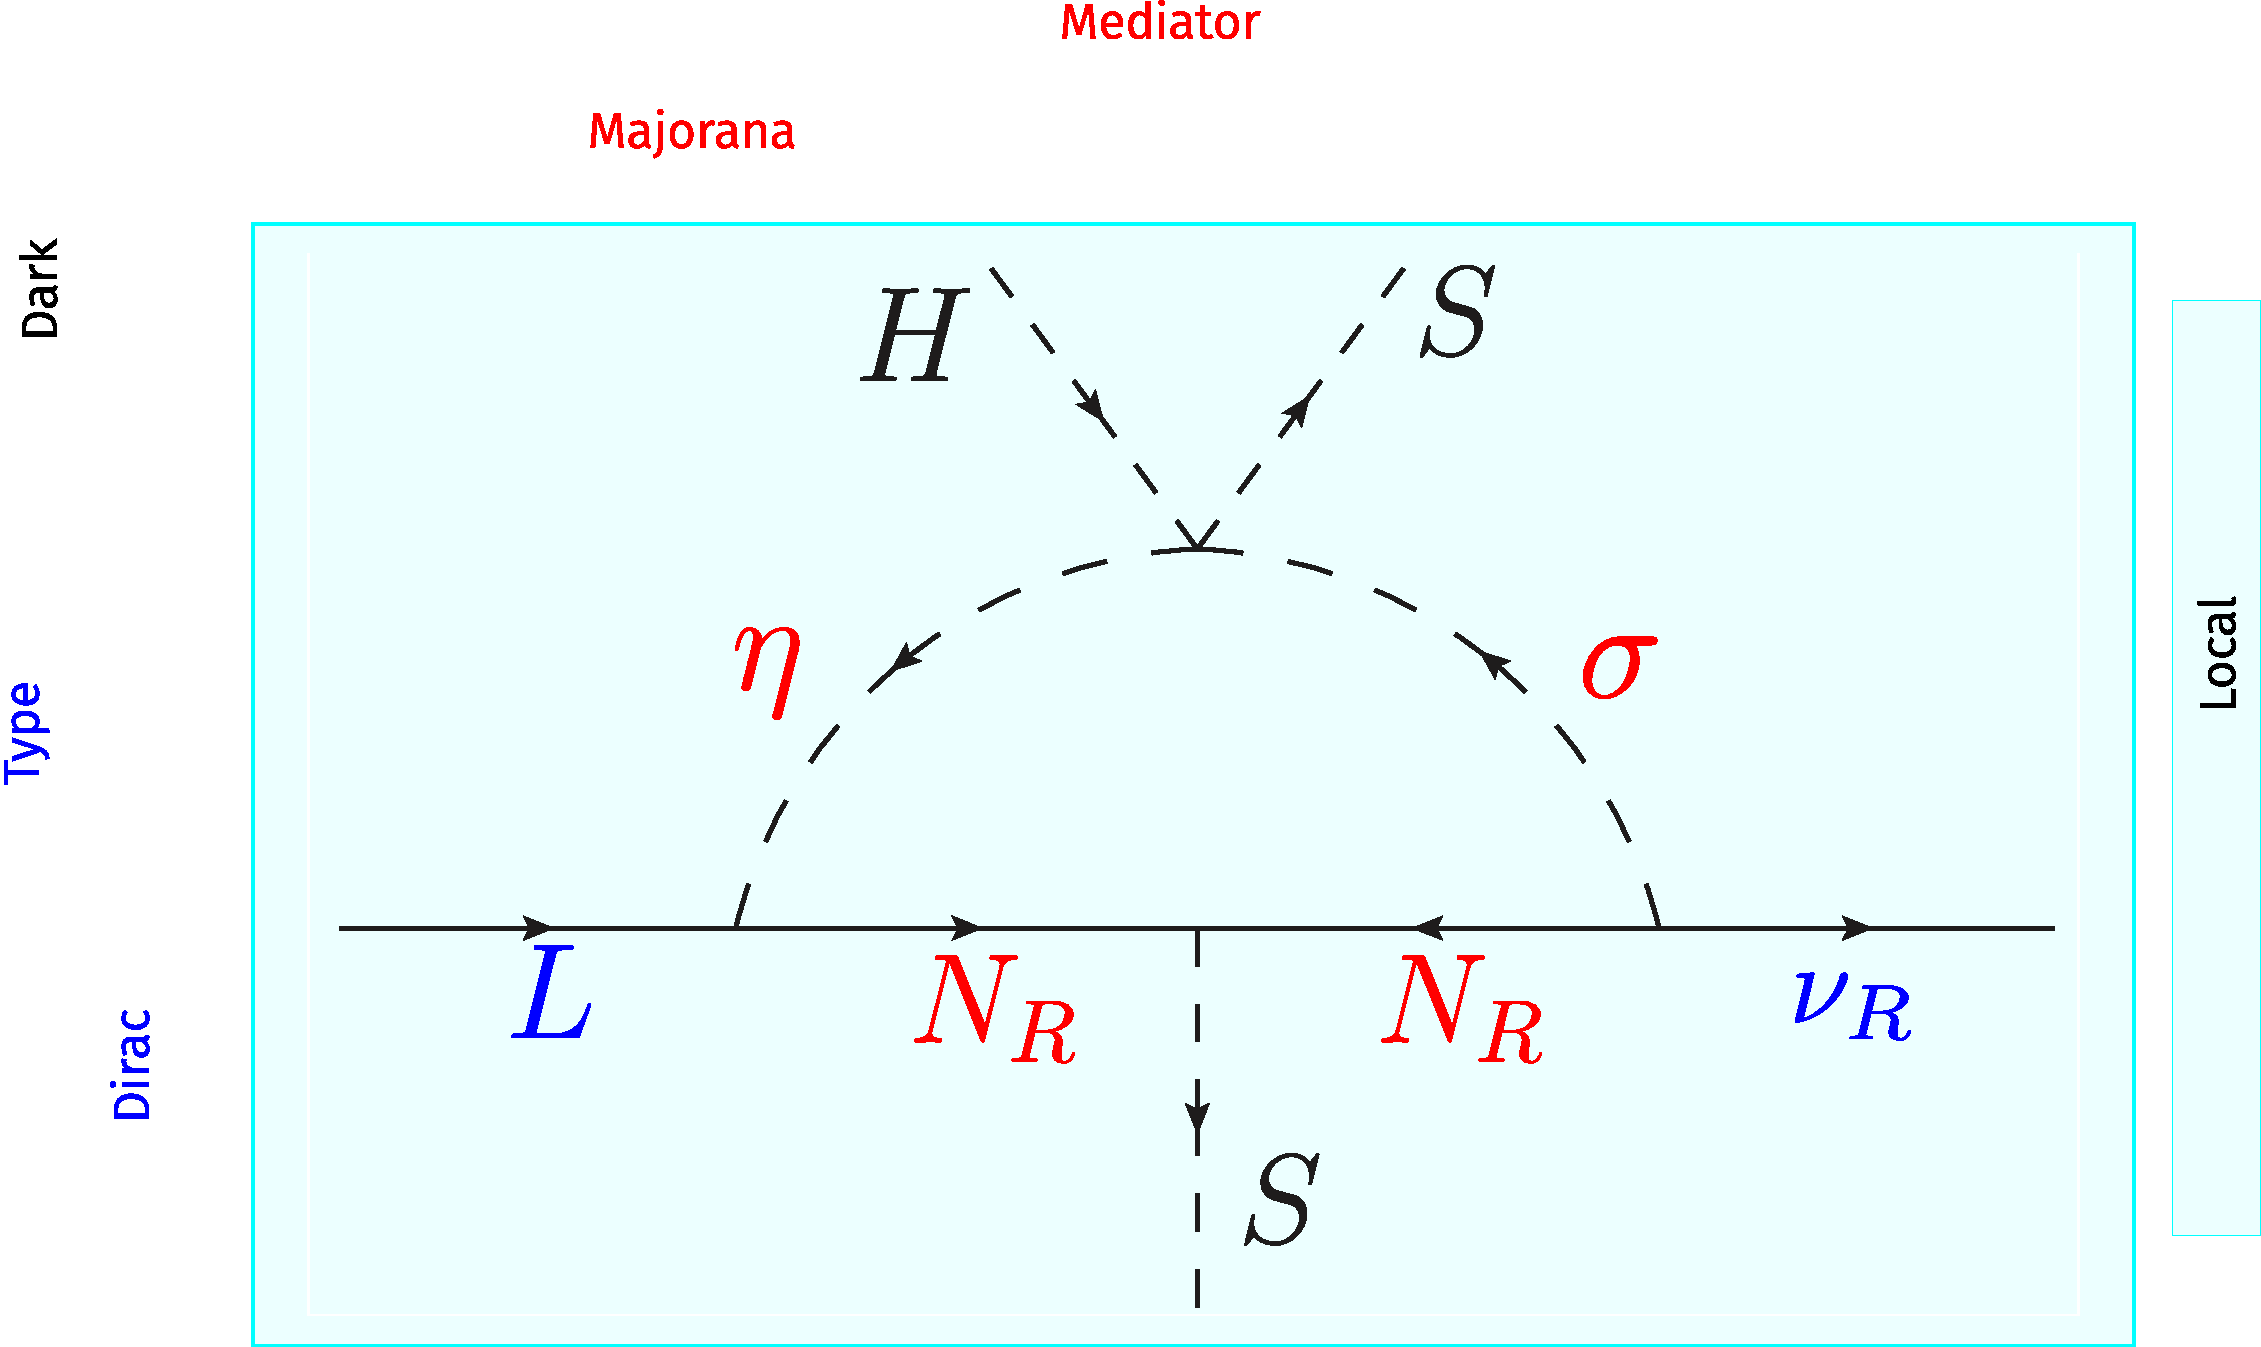
\includegraphics[scale=\rssc]{diracradiativeseesawmajo3}}%
      \only<6>{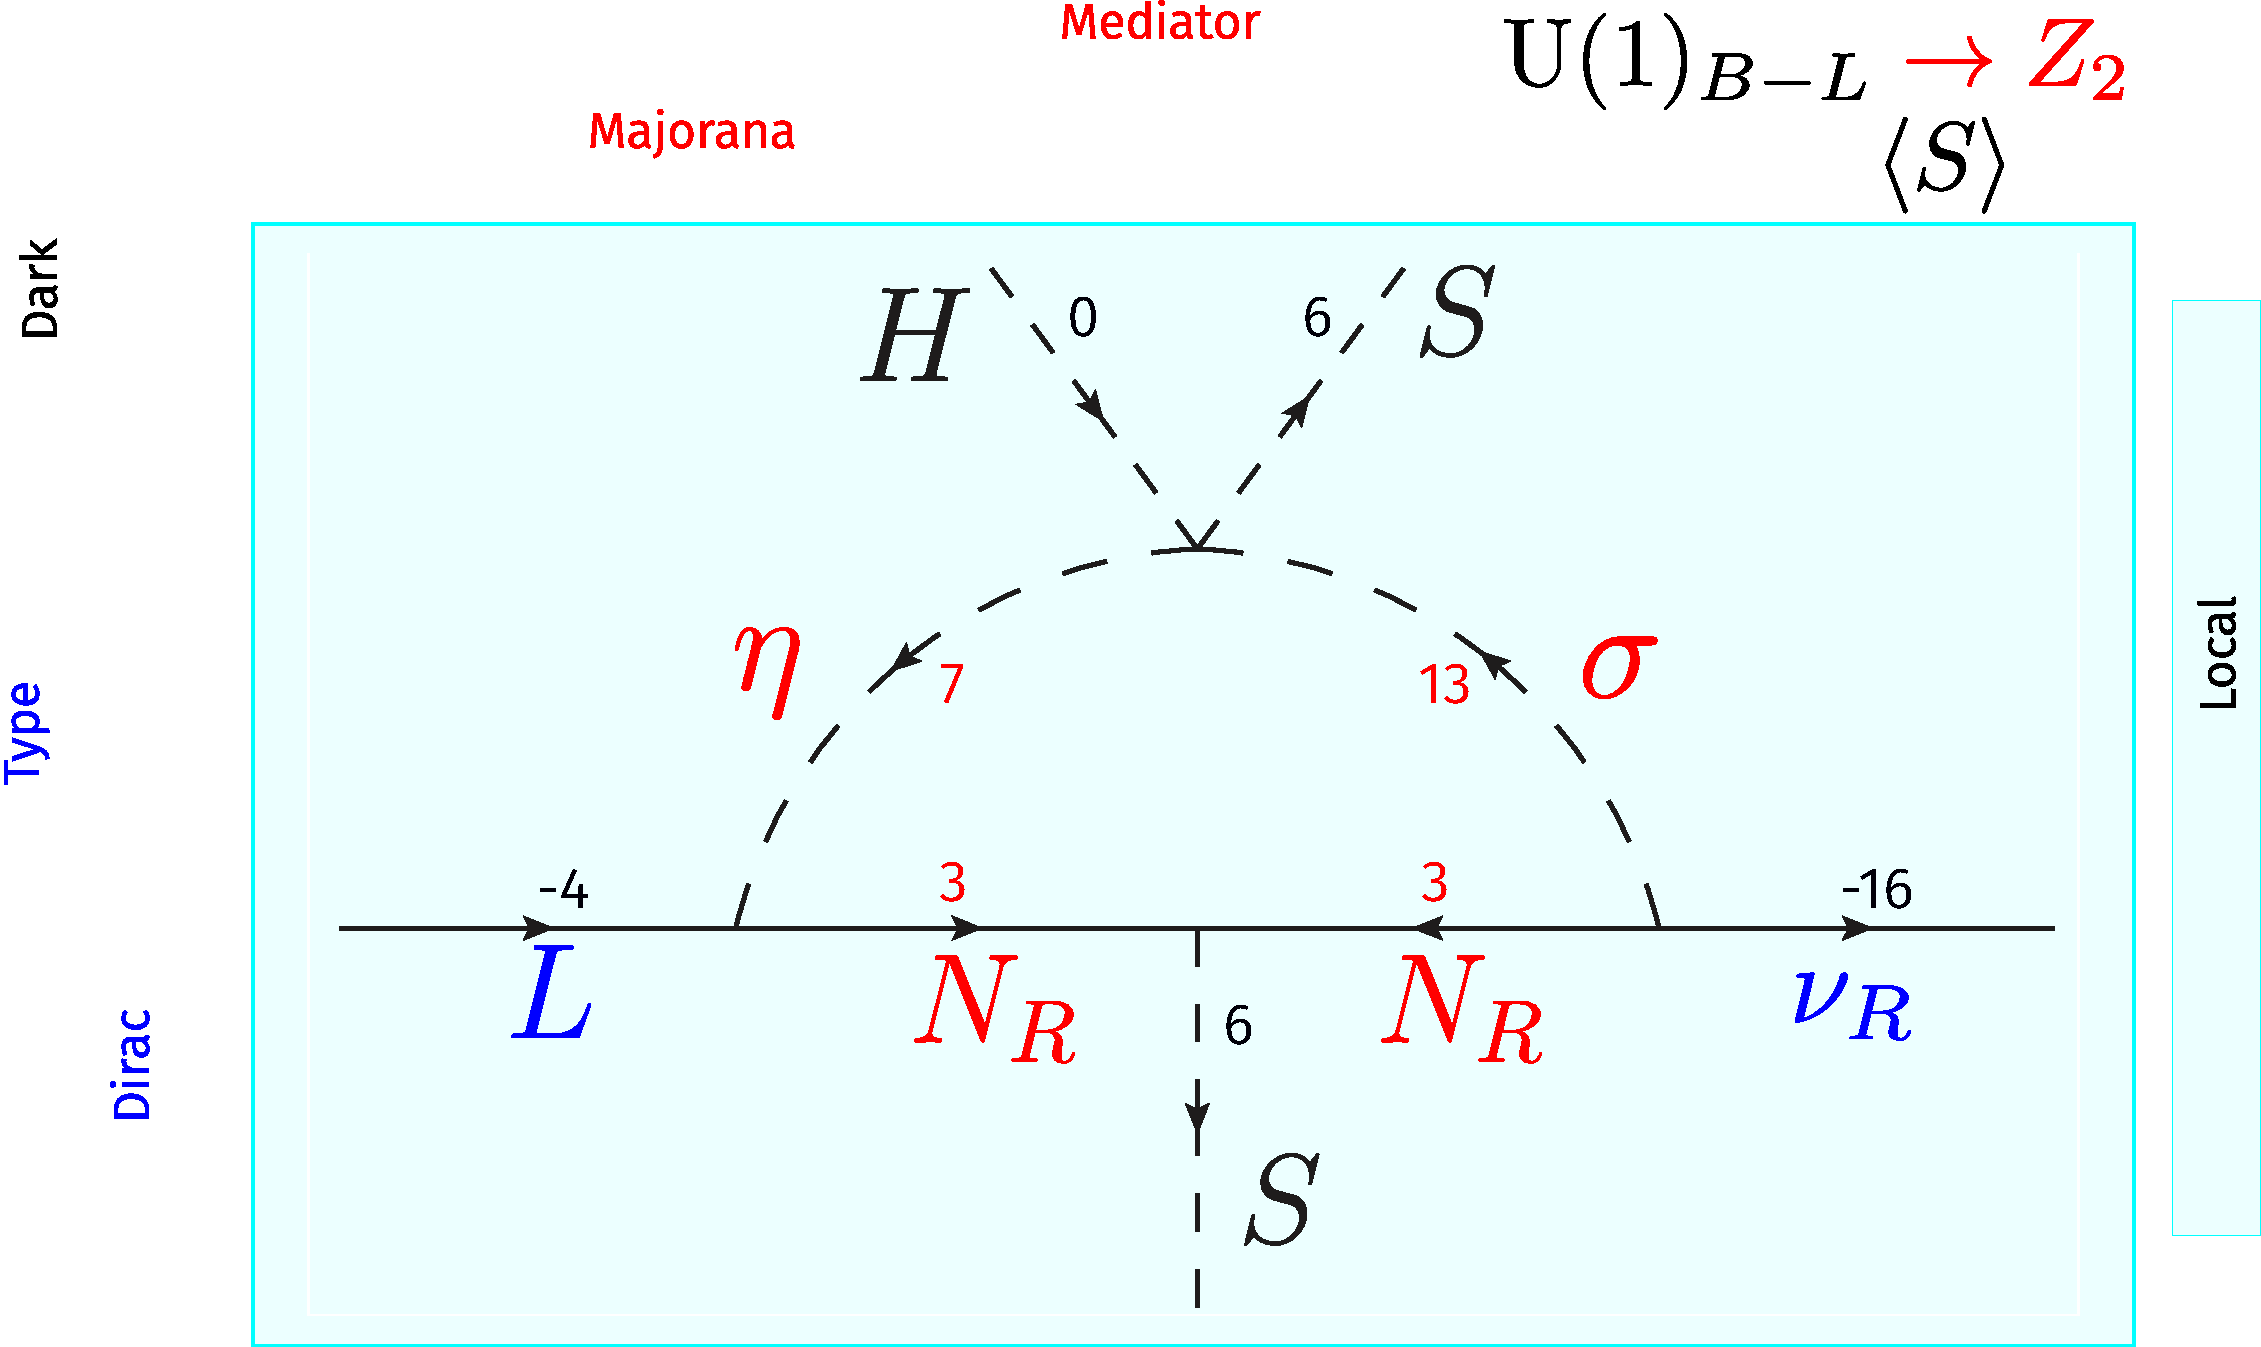
\includegraphics[scale=\rssc]{diracradiativeseesawmajo4}}%
      \invisible<1-2>{
        \begin{align*}
          N=&-\frac{\nu}{4}\invisible<1-4>{-\frac{1}{4}}\,,&\eta=&-\frac{\nu}{4}\invisible<1-4>{-\frac{1}{4}{\color{blue}\only<5>{-l}\only<6->{+1}}}\,,&\sigma=&-\frac{3\nu}{4}\invisible<1-4>{+\frac{1}{4}}\,.
\end{align*}
      }
    \end{column}
    \begin{column}{0.35\textwidth}
      \only<1>{ {\small For radiative Dirac models with only $\operatorname{U}(1)_{X}$ see also: }

        \begin{tiny}
          arXiv:1812.01599,
          1901.06402,
          1902.07259,
          1903.01477,
          1904.07407,
          1907.08630,
             1910.09537
             1909.00833 
          1907.11557,
        1909.09574
          % CO(3) US(3) DE(1) CH(1) ES(3) MX(3)
        \end{tiny}

        $\mathcal{O}(50)$ new models mostly with $\color{red}\sim(-4,-4,5)$
        
        Example: \includegraphics[scale=0.1]{new} $\operatorname{U}(1)_{B-L}$

        \includegraphics[scale=0.6]{T1-2-A}

        {\small Pheno analysis with}

        {\tiny A. Rivera, W. Tangarife,  arXiv:1906.09685 [PRD]}

        \vspace{0.47cm}

        \qquad
        }%
      \only<2->{\invisible<2>{
        \small
        \rowcolors{1}{RoyalBlue!20}{}
  \begin{tabular}{c|c|c|c}
    \hline  
    Fields   & $\operatorname{SU}(2)_L$ & $\operatorname{U}(1)_Y $  & $\operatorname{U}(1)_{  \only<3-4>{\mathcal{D}}\only<5>{X}\only<6->{B-L}   }$\\ \hline
$L $  & $\boldsymbol{2}$& $-1/2$&$\only<1-4>{0}\only<5>{{\color{blue}l}      }\only<6->{-1}$ \\    
$Q $  & $\boldsymbol{2}$& $-1/6$&$\only<1-4>{0}\only<5>{-{\color{blue}l}/3   }\only<6->{1/3}$ \\
$d_R $& $\boldsymbol{1}$& $-1/2$&$\only<1-4>{0}\only<5>{1+2{\color{blue}l}/3 }\only<6->{1/3}$ \\
$u_R $& $\boldsymbol{1}$& $+2/3$&$\only<1-4>{0}\only<5>{-1-4{\color{blue}l}/3}\only<6->{1/3}$ \\
$e_R $& $\boldsymbol{1}$& $-1$  &$\only<1-4>{0}\only<5>{1+2{\color{blue}l}   }\only<6->{-1}$ \\
$H $  & $\boldsymbol{2}$& $1/2$& $\only<1-4>{0}\only<5>{-1-{\color{blue}l}   }\only<6->{0}$\\\hline
$\eta$ & $\boldsymbol{2}$& $1/2$  &$\only<1-4>{1}\only<5>{3/4-\color{blue}l}  \only<6->{7/4}$ \\
$S$ & $\boldsymbol{1}$& $0$ &$\only<1-4>{2}\only<5->{3/2}$ \\    
$\sigma$ & $\boldsymbol{1}$& $0$ &$\only<1-4>{3}\only<5->{13/4}$ \\\hline        
    $\nu_{R1}$& $\boldsymbol{1}$& $0$ & ${-}4$\\
$\nu_{R2}$& $\boldsymbol{1}$& $0$ & ${-}4$\\
$\nu_{R3}$& $\boldsymbol{1}$& $0$ & $5$\\
$N_{R1}$& $\boldsymbol{1}$& $0$ & $\only<1-4>{1}\only<5->{3/4}$\\
$N_{R2}$& $\boldsymbol{1}$& $0$ & $\only<1-4>{1}\only<5->{3/4}$\\
$N_{R3}$& $\boldsymbol{1}$& $0$ & $\only<1-4>{1}\only<5->{3/4}$\\\hline\hline
\only<1-4>{TOTAL}\only<5->{$\xi_{L\alpha}$} &\only<5->{$\boldsymbol{1}$} &\only<5->{$0$}& $\only<1-4>{0}\only<5->{3/4}$ \\
  \end{tabular}
}}%
    \end{column}
  \end{columns}
\end{frame}

\begin{frame}
  \frametitle{The model}
  
\begin{align*}
\label{eq:LagY}
    \mathcal{L} \supset& -\,g^{\prime}\,Z_\mu^\prime\sum_{F}q_{F}\overline{F} \gamma^\mu F+\sum_{\phi}\left|\left( \partial_\mu +i\,g^{\prime}\,q_\phi\,Z'_\mu \right) \phi\right|^2\nonumber\\
    &-[ 
    h_{i\alpha} \overline{L_{i}} \tilde{\eta} N_{R\alpha} +  y_{j\alpha} \overline{\nu_{R_{j}}} \sigma^* N^c_{R\alpha} + k_{\alpha} \overline{N^{c}_{R\alpha}} N_{R\alpha} S^* + \text{h.c.}] - \mathcal{V}(H, S, \eta, \sigma)\,.
\end{align*}
%
 $F$ ($\phi$) denote the new fermions (scalars)
\begin{align*}
%   \label{eq:VHSetasigma}
     \mathcal{V}(H, S, \eta, \sigma) = & V(H) + V(S) + V(\eta) + V(\sigma) \nonumber\\
     &+  \lambda_{HS} (H^{\dagger} H ) (S^{*} S) + \lambda_{2} (H^{\dagger} H ) (\sigma^{*} \sigma ) + \lambda_{3} (H^{\dagger} H ) (\eta^{\dagger} \eta )\nonumber\\
     &+ \lambda_{4} (S^{*} S) (\sigma^{*} \sigma ) + \lambda_{5} (S^{*} S) (\eta^{\dagger} \eta ) + \lambda_{6} (\eta^{\dagger} \eta ) (\sigma^{*} \sigma ) + \lambda_{7} (\eta^{\dagger} H ) (H^{\dagger} \eta ) \nonumber\\
     &+ \lambda_{8} (\eta^{\dagger} H S^{*} \sigma + \text{h.c.})\,,
\end{align*}

\end{frame}

\begin{frame}
  \frametitle{Neutrino masses and LFV}
\begin{align*}
(\mathcal{M}_{\nu})_{ij} = \frac{1}{32 \pi^{2}}  \frac{\lambda_8 v_S^2 v_H} {m_{\eta^0_R}^{2}-m_{\sigma^0_R}^{2}}\sum_{\alpha=1}^{3} h_{i \alpha} k_\alpha y^{*}_{j\alpha}\left[ F\left( \frac{m_{\eta^0_R}^{2}}{M_{N_{\alpha}}^{2}} \right) - F\left( \frac{m_{\sigma^0_R}^{2}}{M_{N_{\alpha}}^{2}} \right) \right] + (R \to I)\,,
\end{align*}
%
where $F(x) =x \log x/(x-1)$. 

\begin{block}{$\mu\to e \gamma$}
  \begin{columns}
    \begin{column}{0.5\textwidth}
\includegraphics[scale=0.5]{LFV}           
    \end{column}
    \begin{column}{0.5\textwidth}
\begin{align*}
    \left| \sum_{\alpha}h_{2 \alpha} h_{1\alpha}^{*} \right| \lesssim 0.02 \left(\frac{m_\chi}{2\,\text{TeV}} \right)^{2}.
\end{align*}
    \end{column}
  \end{columns}
  

  


\end{block}

\end{frame}

\begin{frame}
\begin{picture}(320,250)
\only<1>{\put(-24,-30){\begin{overpic}[scale=0.352]{limits1}\end{overpic}}}%    
\only<2>{\put(-24,-30){\begin{overpic}[scale=0.352]{limits2}\end{overpic}}}%    
\only<3>{\put(-24,-30){\begin{overpic}[scale=0.352]{limits3}\end{overpic}}}%    
\only<4>{\put(-24,-30){\begin{overpic}[scale=0.352]{limits4}\end{overpic}}}%    
\only<5>{\put(-24,-30){\begin{overpic}[scale=0.352]{limits5}\end{overpic}}}%    
\only<6>{\put(-24,-30){\begin{overpic}[scale=0.352]{limits6}\end{overpic}}}%
\only<7>{\put(-24,-30){\begin{overpic}[scale=0.352]{limits7}\end{overpic}}}%    
\end{picture}
\end{frame}

\section{(One-loop) Dirac neutrino masses}

% %slide with sm dirac fermion explanation
% \begin{frame}
%   \frametitle{Lepton number}
%   \begin{itemize}
%   \item   Lepton number ($L$) is an accidental discret or Abelian symmetry of the standard model (SM). 
%   \item  Without neutrino masses $L_e$, $L_{\mu}$, $L_{\tau}$ are also conserved.
%   \item The processes which violates individual $L$ are called Lepton flavor violation (LFV) processes.
%   \item All the neutrino mass models predict, to some extent, LFV processes
%   \item Only models with Majorana neutrinos predict processes with total $L=L_e+L_{\mu}+L_{\tau}$ violation, like \alert{neutrino less doublet beta decay} (NLDBD).
%   \item NLDBD is experimentally challenging, specially if there is a massless neutrino in the spectrum.
%   \end{itemize}
% \end{frame}


% \begin{frame}
%   \frametitle{NLDBD prospects for a  model with \alert{a massless
%     neutrino} \tiny (arXiv:1806.09977 [PLB] with Reig, Valle and Zapata) }
%      \begin{figure}
%       \centering
%       \includegraphics[scale=0.25]{mee}\\
%       {\tiny  with M.Reig, J.W.F Valle, O. Zapata, arXiv:1806.09977  }
%     \end{figure}

 
% \end{frame}


% \begin{frame}
%   \frametitle{Total lepton number: $L=L_e+L_{\mu}+L_{\tau}$}
%   \begin{columns}
%     \begin{column}{0.48\textwidth}
%       \begin{block}{\centering Majorana $\cancel{\operatorname{U}(1)_L}$}
%               \centering
%     \rowcolors{1}{RoyalBlue!20}{}
% \begin{tabular}{cc}
%   Field &  $Z_2\ (\omega^2=1)$ \\\hline
%   SM & $1$\\
%   $L$& $\omega$ \\
%      $ \left( e_R \right)^{\dagger}  $& $\omega$ \\
%     $\left( \nu_R \right)^{\dagger}$ & $\omega$ \\\hline
%     \end{tabular}

%     \begin{align*}
%       \mathcal{L}_{\nu}=h_D \left( \nu_R \right)^{\dagger}L \cdot H +
% {\color{red}M_R\,\nu_R \nu_R}
%       +\text{h.c}\,.
%     \end{align*}
%     \begin{align*}
%       h_D \sim  \mathcal{O}(1) 
%     \end{align*}
%     \invisible<1->{Explain smallness ala Peccei-Quinn:
%     \vspace{-0.5cm}
%     \begin{align*}
%       \operatorname{U}(1)_{B-L}\to Z_N\,,\quad N\ge 3\,.
%     \end{align*}}    

%       \end{block}
%     \end{column}
%   \begin{column}{0.48\textwidth}
%     \begin{block}{\centering Dirac $\only<1>{\operatorname{U}(1)_L}
%         \only<2>{\operatorname{U}(1)_{B-L}}$}
%               \centering
%     \rowcolors{1}{RoyalBlue!20}{}
% \begin{tabular}{cc}
%   Field &  $Z_3\ (\omega^3=1)$ \\\hline
%   SM & $1$\\
%   $L$& $\omega$ \\
%        $ \left( e_R \right)^{\dagger}  $& $\omega^2$ \\
%     $\left( \nu_R \right)^{\dagger}$ & $\omega^2$ \\\hline
%     \end{tabular}

%     \begin{align*}
%       \mathcal{L}_{\nu}=h_D \left( \nu_R \right)^{\dagger}L \cdot H 
%       +\text{h.c}\,.
%     \end{align*}
%     \begin{align*}
%       h_D \sim \mathcal{O}(10^{-11}) 
%     \end{align*}
%     \invisible<1>{Explain smallness ala Peccei-Quinn:
%       \vspace{-0.5cm}
%     \begin{align*}
%       \operatorname{U}(1)_{B-L} \underbrace{\longrightarrow}_{\color{red}\left\langle S \right\rangle} Z_N\,,\quad N\ge 3\,.
%     \end{align*}}    
%       \end{block}
    
%   \end{column}
% \end{columns}

% \end{frame}



\begin{frame} 
  \frametitle{Small Dirac neutrino masses}
  \begin{columns}
    \begin{column}{0.78\textwidth}
      \small \qquad
      
      \vspace{0.2cm}
      
  To explain the \alert{smallness} of Dirac neutrino masses choose $\operatorname{U}(1)_{X} $ which:
  \begin{itemize}
  \item<1-> Forbids tree-level mass (TL) term ( $Y(H)=+1/2$ )
    \begin{align*}
      \mathcal{L}_{\text{T.L}}=&h_{D}\epsilon_{ab} \left( \nu_R \right)^{\dagger} L^a H^b +\text{h.c}\\
      =&h_D\left( \nu_R \right)^{\dagger} L\cdot  H +\text{h.c}\\
    \end{align*}
    \vspace{-1.5cm}
  \item<2-> Forbids Majorana term: $\nu_R \nu_R$
        \vspace{-0.3cm}
   \item<3-> Realizes of the 5-dimension operator which conserves lepton number in    $\operatorname{SU}(3)_c \times\operatorname{SU}(2)_L\times \operatorname{U}(1)_Y\times \operatorname{U}(1)_{B-L}$:
     \begin{align*}
       \mathcal{L}_{5-D}= \frac{h_\nu }{\Lambda}\left( \nu_R \right)^{\dagger} L\cdot H
       {\color{red}S}+\text{h.c}\\
     \end{align*}
             \vspace{-0.3cm}
           \item<4-> Enhancement to the \emph{effective number of degrees of freedom in the early Universe} $\Delta N_{\text{eff}}=N_{\text{eff}}-N_{\text{eff}}^{\text{SM}}$ ({\tiny see arXiv:1211.0186})             
  \end{itemize}

  \invisible<1-3>{See E. Ma, Rahul Srivastava: arXiv:1411.5042 [PLB] for tree-level realization} 
    \end{column}
    \begin{column}{0.22\textwidth}
      \invisible<1-2>{\includegraphics[scale=0.2]{l5d}}
    \end{column}
  \end{columns}

\end{frame}

\begin{frame}
  \frametitle{From {1210.6350} and
    {1805.02025}: $\Delta N_{\text{eff}}=3 \left( T_{\nu_R}/T_{\nu_L} \right)^4$    }
  \begin{columns}
    \begin{column}{0.5\textwidth}
      \footnotesize
      \begin{align*}
{\color{blue} \Gamma_{\nu_R}(T)}&=n_{\nu_R}(T)\sum_f \langle \sigma_f(\nu_R \bar{\nu}_R\to f\bar{f})v \rangle \\ 
&= \sum_f \frac{g_{\nu_R}^2}{n_{\nu_R}}\int \frac{d^3 p }{(2\pi)^3} \frac{d^3 q }{(2\pi)^3}
f_{\nu_R}(p)f_{\nu_R}(q) \sigma_f(s) (1-\cos\theta),
      \end{align*}
\vspace{-0.5cm}      
      \begin{align*}
        s=&2pq(1-\cos\theta),& f_{\nu_R}(k)=& 1/(e^{k/T}+1)\\
        n_{\nu_R}(T)=&g_{\nu_R}\int \frac{d^3k}{(2\pi)^3}f_{\nu_R}(k),& \text{with } g_{\nu_R}=&2\\
        \sigma_f(s)\simeq&\frac{ N_C^f ( { \only<1>{\color{black}}\only<2>{\color{red}}  Q_{BL}^f}   )^2 Q^2 s}{12\pi}\left(\frac{g'}{M_{Z'}}\right)^4,&
       \text{In the limit } M^2_{Z'}\gg& s\,.
      \end{align*}
with three right-handed neutrinos, the Hubble parameter is 
\begin{equation*}
  {\color{blue}H(T)}=\sqrt{\frac{4\pi^3G_N \left[ {  \only<1>{\color{red}}\only<2>{\color{black}}  g(T)}+{21}/{4} \right]}{45}}\,T^2.
\end{equation*}

The right-handed neutrinos decouple when
\begin{align*}
  \color{blue}
  \Gamma_{\nu_R}(T^{\nu_R}_\text{dec})=H(T^{\nu_R}_\text{dec}).
\end{align*}

    \end{column}
    \begin{column}{0.5\textwidth}
      \centering
      \invisible<1>{\includegraphics[scale=0.14]{tree-level-dirac-seesaw}

      {\scriptsize
          \rowcolors{1}{RoyalBlue!20}{}
  \begin{tabular}{cccccc}\hline
   $ \nu_{R3} $
  &$\nu_{R2} $&$\nu_{R1}$&$\psi_L$&$ \psi_R  $&$S$\\ \hline
  $\color{red}-4$&$\color{red}-4$&$\color{red}+5$& $\color{black}-1$ & $\color{black}-1$ & $+3$\\\hline
  \end{tabular}

  {\tiny E. Ma, R. Srivastava: arXiv:1411.5042 [PLB]}
}}
\def\scf{4.9cm}
\only<1>{\includegraphics[height=4.5cm]{gT}

  {\tiny A. Solaguren-Beascoa, M. C. Gonzalez-Garcia: arXiv:{\color{red}1210.6350} [PLB]

\qquad
  }
}%
\only<2->{%
\only<2>{ \includegraphics[height=\scf]{D_Neff}}%
%\only<3->{\includegraphics[height=\scf]{u1blc}}

  {\tiny with J. Calle and Ó. Zapata, arXiv:1909.09574

%    (also: Planck 1807.06209, Riess \emph{et al} 1903.07603 )
  }
}
    \end{column}
  \end{columns}
\end{frame}

%\section{Dark symmetry}



\begin{frame}
  \frametitle{Same constraints as before}
  \only<1>{\includegraphics[height=8cm]{u1blc1}}%
  \only<2>{\includegraphics[height=8cm]{u1blc2}}%
  \only<3>{\includegraphics[height=8cm]{u1blc3}}%
  \only<4>{\includegraphics[height=8cm]{u1blc4}}%
  \only<5->{\includegraphics[height=8cm]{u1blc5}}%  
\end{frame}

\begin{frame}
\frametitle{Conclusions}
  It makes sense to focus our attention on models tha can account for neutrino masses and dark matter (DM) \alert{without adhoc symmetries}
\only<1>{
  \begin{block}{One-loop Dirac neutrino masses}
      A single $U(1)_X$ gauge symmetry to explain both the smallnes of Dirac neutrino masses and the stability of Dirac fermion dark matter
  %\setbeamercolor{block body}{use=structure,fg=black,bg=white}
    \begin{itemize}
    \item Spontaneously broken $U(1)_{X}$ generates a radiative Dirac neutrino masses
  \item A remnant symmetry makes the lightest field circulating the loop stable and good dark matter candidate.
  \item For T1-2-A: Either Singet Doublet Dirac Dark Matter or Singlet Scalar Dark Matter with extra scalar and vector portal
  \item Dark symmetry for Majorana mediatiors
    \end{itemize}
  \end{block}
}

\end{frame}





{
%\usebackgroundtemplate{\includegraphics[height=\paperheight]{silafaegua}}    
  \plain{
  %\only<2>{\includegraphics[scale=0.9]{slfg}}
  
  Thanks!}
}
\end{document}


%slide with sm dirac fermion explanation
\begin{frame}
  \frametitle{Lepton number}
  \begin{itemize}
  \item   Lepton number ($L$) is an accidental discret or Abelian symmetry of the standard model (SM). 
  \item  Without neutrino masses $L_e$, $L_{\mu}$, $L_{\tau}$ are also conserved.
  \item The processes which violates individual $L$ are called Lepton flavor violation (LFV) processes.
  \item All the neutrino mass models predict, to some extent, LFV processes
  \item Only models with Majorana neutrinos predict processes with total $L=L_e+L_{\mu}+L_{\tau}$ violation, like \alert{neutrino less doublet beta decay} (NLDBD).
  \item NLDBD is experimentally challenging, specially if there is a massless neutrino in the spectrum.
  \end{itemize}
\end{frame}

%\end{document}
\begin{frame}
  \frametitle{NLDBD prospects for a  model with a massless
    neutrino \tiny (arXiv:1806.09977 [PLB] with Reig, Valle and Zapata) }
     \begin{figure}
      \centering
      \includegraphics[scale=0.25]{mee}\\
      {\tiny  with M.Reig, J.W.F Valle, O. Zapata, arXiv:1806.09977  }
    \end{figure}

 
\end{frame}


\begin{frame}
  \frametitle{Total lepton number: $L=L_e+L_{\mu}+L_{\tau}$}
  \begin{columns}
    \begin{column}{0.48\textwidth}
      \begin{block}{\centering Majorana $\cancel{\operatorname{U}(1)_L}$}
              \centering
    \rowcolors{1}{RoyalBlue!20}{}
\begin{tabular}{cc}
  Field &  $Z_2\ (\omega^2=1)$ \\\hline
  SM & $1$\\
  $L$& $\omega$ \\
     $ \left( e_R \right)^{\dagger}  $& $\omega$ \\
    $\left( \nu_R \right)^{\dagger}$ & $\omega$ \\\hline
    \end{tabular}

    \begin{align*}
      \mathcal{L}_{\nu}=h_D \left( \nu_R \right)^{\dagger}L \cdot H +
{\color{red}M_R\,\nu_R \nu_R}
      +\text{h.c}\,.
    \end{align*}
    \begin{align*}
      h_D \sim  \mathcal{O}(1) 
    \end{align*}
    \invisible<1->{Explain smallness ala Peccei-Quinn:
    \vspace{-0.5cm}
    \begin{align*}
      \operatorname{U}(1)_{B-L}\to Z_N\,,\quad N\ge 3\,.
    \end{align*}}    

      \end{block}
    \end{column}
  \begin{column}{0.48\textwidth}
    \begin{block}{\centering Dirac $\only<1>{\operatorname{U}(1)_L}
        \only<2>{\operatorname{U}(1)_{B-L}}$}
              \centering
    \rowcolors{1}{RoyalBlue!20}{}
\begin{tabular}{cc}
  Field &  $Z_3\ (\omega^3=1)$ \\\hline
  SM & $1$\\
  $L$& $\omega$ \\
       $ \left( e_R \right)^{\dagger}  $& $\omega^2$ \\
    $\left( \nu_R \right)^{\dagger}$ & $\omega^2$ \\\hline
    \end{tabular}

    \begin{align*}
      \mathcal{L}_{\nu}=h_D \left( \nu_R \right)^{\dagger}L \cdot H 
      +\text{h.c}\,.
    \end{align*}
    \begin{align*}
      h_D \sim \mathcal{O}(10^{-11}) 
    \end{align*}
    \invisible<1>{Explain smallness ala Peccei-Quinn:
      \vspace{-0.5cm}
    \begin{align*}
      \operatorname{U}(1)_{B-L} \underbrace{\longrightarrow}_{\color{red}\left\langle S \right\rangle} Z_N\,,\quad N\ge 3\,.
    \end{align*}}    
      \end{block}
    
  \end{column}
\end{columns}

\end{frame}



\begin{frame} 
  \frametitle{Small Dirac neutrino masses}
  \begin{columns}
    \begin{column}{0.78\textwidth}
      \small \qquad
      
      \vspace{0.2cm}
      
  To explain the \alert{smallness} of Dirac neutrino masses choose $\operatorname{U}(1)_{B-L} $ which:
  \begin{itemize}
  \item<1-> Forbids tree-level mass (TL) term ( $Y(H)=+1/2$ )
    \begin{align*}
      \mathcal{L}_{\text{T.L}}=&h_{D}\epsilon_{ab} \left( \nu_R \right)^{\dagger} L^a H^b +\text{h.c}\\
      =&h_D\left( \nu_R \right)^{\dagger} L\cdot  H +\text{h.c}\\
    \end{align*}
    \vspace{-1.5cm}
  \item<2-> Forbids Majorana term: $\nu_R \nu_R$
        \vspace{-0.3cm}
   \item<3-> Realizes of the 5-dimension operator which conserves lepton number in    $\operatorname{SU}(3)_c \times\operatorname{SU}(2)_L\times \operatorname{U}(1)_Y\times \operatorname{U}(1)_{B-L}$:
     \begin{align*}
       \mathcal{L}_{5-D}= \frac{h_\nu }{\Lambda}\left( \nu_R \right)^{\dagger} L\cdot H
       {\color{red}S}+\text{h.c}\\
     \end{align*}
             \vspace{-0.3cm}
           \item<4-> Enhancement to the \emph{effective number of degrees of freedom in the early Universe} $\Delta N_{\text{eff}}=N_{\text{eff}}-N_{\text{eff}}^{\text{SM}}$ ({\tiny see arXiv:1211.0186})             
  \end{itemize}

  \invisible<1-3>{See E. Ma, Rahul Srivastava: arXiv:1411.5042 [PLB] for tree-level realization} 
    \end{column}
    \begin{column}{0.22\textwidth}
      \invisible<1-2>{\includegraphics[scale=0.2]{l5d}}
    \end{column}
  \end{columns}

\end{frame}



\begin{frame}
\begin{picture}(320,250)
\only<1->{\put(-24,-22){\begin{overpic}[scale=0.352]{z2_bkg}\end{overpic}}}%
\only<1->{\put(34,158.5){ \textbf{SM}  }}%
\only<1->{\put(38,115){ {\large +}  }}%
\only<1->{\put(0,100){\Large $m^{\nu}_{\text{Majorana}}=\frac{1}{\Lambda} L \cdot H L \cdot H$   }}%
\only<1->{\put(-10,80){\Large $m^{\nu}_{\text{Dirac}}=\frac{1}{\Lambda} \left( \nu_R \right)^{\dagger}L \cdot H S$  }}%
%\only<2->{\put(2,80){ {\scriptsize This work, arXiv:1308.3655  [JHEP]} }}%
\only<1->{\put(18,115){\begin{overpic}[scale=0.118]{mice}\end{overpic}}}%
%
\only<2->{\put(240,180){\begin{overpic}[scale=0.15]{brickY}\end{overpic}}}%
\only<2->{\put(310,180){\begin{overpic}[scale=0.15]{brickR}\end{overpic}}}%
\only<2->{\put(380,180){\begin{overpic}[scale=0.15]{brickB}\end{overpic}}}%
\only<2->{\put(190,120){\begin{overpic}[scale=0.15]{brickG}\end{overpic}}}%
\only<2->{\put(260,120){\begin{overpic}[scale=0.15]{brickW}\end{overpic}}}%
\only<2->{\put(330,120){\begin{overpic}[scale=0.15]{brickK}\end{overpic}}}%
\only<2->{\put(120,40){ \begin{overpic}[scale=0.15]{brickssY}\end{overpic}}}%
\only<2->{\put(190,40){ \begin{overpic}[scale=0.15]{brickssR}\end{overpic}}}%
\only<2->{\put(260,40){ \begin{overpic}[scale=0.15]{brickssB}\end{overpic}}}%
\only<2->{\put(90,0){ \begin{overpic}[scale=0.15]{brickssG}\end{overpic}}}%
\only<2->{\put(160,0){ \begin{overpic}[scale=0.15]{brickssW}\end{overpic}}}%
\only<2->{\put(230,0){ \begin{overpic}[scale=0.15]{brickssK}\end{overpic}}}%
%\only<3->{\put(70,158){ \begin{overpic}[scale=0.27]{alert}\end{overpic}}}%
%\only<3->{\put(90,195){ {\huge \textbf{35 models}}  }}%
\end{picture}
\end{frame}


\end{document}

\begin{frame}
  \frametitle{\includegraphics[scale=0.1]{Q} \qquad Colored dark matter:
  \small De Luca , Mitridate, Redi, Smirnov \& Strumia, \tiny arXiv:1801.01135 [PRD]}

(Switch to Dirac fermions) \\
Because $\mathcal{Q}$ is a Dirac fermion, $\mathcal{Q} \mathcal{Q}$ is also stable
\begin{align*}
  \mathcal{Q}\mathcal{Q}\, \cancel{\to} &\, g\,, &\overline{\mathcal{Q}}\overline{\mathcal{Q}}\, \cancel{\to} &\, g\,.
\end{align*}

    \includegraphics[scale=0.09]{dmsteps}
  
\end{frame}


\begin{frame}
  \frametitle{Relic abundance. \footnotesize From: \url{http://bit.ly/Mitridate_53d_53rd_Rencontres_de_Moriond}  }
  \includegraphics[scale=0.3]{relden} 
\end{frame}

\begin{frame}
  \frametitle{Direct detection}
  \includegraphics[scale=0.52]{sigmaSI}
\end{frame}



\begin{frame}
  \frametitle{\only<1->{
    SD${}^{3}$M+$\sigma_i$ ($i=1,2$)     \invisible<2>{\scriptsize with J. Calle, C. Yaguna, and O. Zapata, arXiv:1812.05523 [PRD]  }  }}
\begin{picture}(320,250)
\only<1>{\put(-20,130){\tiny
        \begin{minipage}{0.3\linewidth}
          \begin{align*}
            \psi_{L,R}\to&\text{Singlet fermions \only<1>{(quiral)}  }\\
            \only<1>{\Psi_{L,R}\to&\text{Vector-like doublet fermions}\only<1>{:\qquad {\color{red}10/5}}   }\\
            \sigma\to&\text{Singlet scalar}\only<1->{:\qquad 15/5}   \\
            %\only<1>{\eta\to&\text{Doublet scalar}   }
          \end{align*}
        \end{minipage}
}}%
\only<1>{\put(190,135){\tiny
    \begin{minipage}{0.3\linewidth}
      \rowcolors{1}{RoyalBlue!20}{}
  \begin{tabular}{c|ccccccccc}\hline
 Fields: $f_i$  &  $\left( \nu_{R3} \right)^{\dagger}$
  &$\left( \nu_{R2} \right)^{\dagger}$&$\left( \nu_{R1} \right)^{\dagger}$&$\psi_L$&$\left( \psi_R \right)^{\dagger}$&$S$ &$\Psi_L$ & $\widetilde{\left( \Psi_R \right)}$& $\sigma$\\ \hline
    $\operatorname{U}(1)_{B-L}$ &$\displaystyle{+\frac{8}{5}}$&$\displaystyle{+\frac{8}{5}}$&$\displaystyle{+\frac{2}{5}}$&$\displaystyle{\frac{7}{5}}$&$\color{red}\displaystyle{-\frac{10}{5}}$&$\color{blue}\displaystyle{+\frac{3}{5}}$ &$\displaystyle{\frac{10}{5}}$ & $\displaystyle{-\frac{10}{5}}$  & $\displaystyle{\frac{7}{5}}$\\
    $\operatorname{SO}(10)$ &$16$ & $16$ & $16$ & $45$ & $45$ & $126$ & $10$ &$10$ & $16$ \\
  \end{tabular}
         \end{minipage}
       }}%
\only<1>{\put(250,95){\tiny
    \begin{minipage}{0.3\linewidth}
      \begin{center}
        Second Scotogenic Dirac from $\operatorname{SO}(10)$ E. Ma arXiv:1901.09091 [PLB]
       \end{center}
       \end{minipage}
       }}%
%  effective number of relativistic degrees of reedom Neff for neutrinos
% \only<4>{\put(40,20){\begin{overpic}[scale=0.6]{radiativedirac4}\end{overpic}}}%
 \only<1->{\put(40,20){\begin{overpic}[scale=0.6]{radiativedirac5}\end{overpic}}}%
 \only<2>{\put(20,200){
     \begin{minipage}{0.3\linewidth}
       $M_\psi=h_1 \left\langle S \right\rangle$, $\color{red}y_2=0$:
          \begin{align*}
            \mathcal{L}={\color{red}\mathcal{L}_{\text{SD${}^3$M}}}
            +{\color{Green} h_3^{ia} \widetilde{\left( \Psi_R \right)}\cdot L_i\, \sigma_a}+
      {\color{blue}      h_2^{\beta a} \left( \nu_{R\beta} \right)^{\dagger} \psi_L\, \sigma^{*}_a}
            -V(\sigma_a,S,H)\,.
          \end{align*}
        \end{minipage}
}}%
\only<2>{\put(0,130){\small with A.F Rivera, W. Tangarife,  arXiv:1906.09685   }}%
\only<2>{\put(220,60){\begin{overpic}[scale=0.6]{sarah}\end{overpic}}}%
\end{picture}
\end{frame}


% Now we introduce a vector like doublet
% From now on we will also decouple the Z'
% we end up with


\begin{frame}
  \frametitle{ Singlet-Doublet Dirac Dark Matter (SD${}^{3}$M)
By Carlos E. Yaguna.
arXiv:1510.06151 [PRD].
}

The model extends the standard model (SM) particle content with Dirac Fermions: from  $\operatorname{SU}(2)$ doublets of Weyl fermions: $\Psi_L=\left( \Psi_L^0,\, \Psi_L^-\right)^{\operatorname{T}}$, $\widetilde{\left( \Psi_R \right)}=\left( (\Psi_R^-)^\dagger,\, -(\Psi_R^0)^\dagger\right)^{\operatorname{T}}$  and singlet Weyl fermions $\psi_{LR}$ that interact among themselves and with the SM fields 
\begin{align}
  \mathcal{L}\supset& {\color{red} M_{\psi}}\left( \psi_R \right)^{\dagger}\psi_L
%+ {\color{red}h_S} \left( \psi_R \right)^{\dagger} \psi_LS  %+\text{h.c}.
%  \mathcal{L}_{\psi}+\mathcal{L}_{\sigma\psi}
+ %\left[
{\color{red}M_{\Psi}}\widetilde{\left( \Psi_R \right)}\cdot  \Psi_L
% +h_2^{ia} \widetilde{\left( \Psi_R \right)}\cdot L_i\, \sigma_a
+ {\color{red} y_1} \left( \psi_R \right)^{\dagger} \Psi_L \cdot H
+ {\color{red} y_2}  \widetilde{\left( \Psi_R \right)} \cdot \widetilde{H} \psi_L
                      +\text{h.c} % \right]
%+V(\sigma_a,S,H)\,,
\end{align}
Four free parameters:
\begin{align}
  {\color{red} M_{\psi}},{\color{red}M_{\Psi}}\ <& 2\text{ GeV}\,,&
  {\color{red} y_1},\ {\color{red} y_2} > 10^{-6}
\end{align}
Two neutral Dirac fermion eigenstates:
\begin{align}
  M=&
  \begin{pmatrix}
    {\color{red}M_{\psi}} & {\color{red}y_{2}} v/\sqrt{2} \\ {\color{red}y_{1}} v/\sqrt{2} & {\color{red} M_{D}}
  \end{pmatrix},&
M_{\text{diag}}=&
\begin{pmatrix}
{M_{\chi_{1}}} & {0} \\ {0} & {M_{\chi_{2}}}                    
\end{pmatrix}
=U_{L}^{\dagger} M U_{R}
\end{align}


\end{frame}


\begin{frame}
    \frametitle{ SD${}^{3}$M
By Carlos E. Yaguna.
arXiv:1510.06151 [PRD].
}
    \begin{columns}
    \begin{column}{0.5\textwidth}
      \includegraphics[scale=0.24]{coannmass}

    \hspace{2cm} Compressed spectra region
   \end{column}
    \begin{column}{0.5\textwidth}
      \includegraphics[scale=0.24]{ddsi}

      \only<1-2>{\hspace{2cm}LUX - XENON1T - LZ}
    \end{column}

  \end{columns}
  
  \invisible<1>{\includegraphics[scale=0.2]{llcom}}
  
  
\end{frame}


\begin{frame}
  \frametitle{Spin independent (SI) direct detection cross section}
  \begin{columns}
    \begin{column}{0.5\textwidth}
      
\includegraphics[scale=0.4]{vector-SI}
\includegraphics[scale=0.4]{scalar-SI}

\scriptsize Decoupled $Z'$ limit
    \end{column}
    \begin{column}{0.5\textwidth}
\includegraphics[scale=0.4]{MSvsMD}

\scriptsize Vector SI (blue points) and  scalar SI (green points)      
    \end{column}
  \end{columns}
\end{frame}

%\begin{frame}
%   \frametitle{SM-like $B-L$ model}
%  \begin{center}
%     \rowcolors{1}{RoyalBlue!20}{}
%  \begin{tabular}{lr}
%    Field & $\operatorname{U}(1)_{B-L}$ \\ \hline
%    $L$   & -1\\
%    $H$   & 0\\
%    $S$   & $s$\\
%    $\left( \psi_R \right)^{\dagger}_\alpha$ & $\color{red}r_{\alpha}$\footnote{Weyl notation with only left-handed fields defined; $\color{red}r_{\alpha}$ restricted by anomaly cancellation}\\
%  \end{tabular}
% \end{center}

% \begin{block}{Massless Majorana fermions ($n=0,1$)}
%   \begin{align*}
%     L \left[ \left( \psi_R \right)^{\dagger}_\alpha \left( \psi_R \right)^{\dagger}_\beta S^n \right]  \Longrightarrow& {\color{red} r_{\alpha}+r_{\beta}}+nS\ne 0\,,
%    & &\text{example: $\color{red}r\ne 1$, if $s=-2$}\,.
%   \end{align*}
% \end{block}

%  \vspace{-0.5cm}
% \setbeamercolor{block title}{bg=yellow!30,fg=black}
%  \begin{varblock}[\textwidth]{  $\operatorname{U}(1)_{B-L}$ with 3+$\alpha$ zero Majorana Masses $\iff$ SM with 3 zero Majorana masses }      
%  \end{varblock}

% \vspace{-0.8cm}
%  \begin{align*}
% \text{ For $\alpha\le 2$: }   \left( \psi_R \right)^{\dagger}_\alpha\to &\left( \nu_R \right)^{\dagger}_\alpha&
%           \color{red} r_{\alpha}\to & \color{Green} \nu_{\alpha}
%  \end{align*}


 

 
% \end{frame}

%\end{document}

% \begin{frame}
%   \frametitle{Majorana vs Dirac}
%   \begin{columns}
%     \begin{column}{0,5\textwidth}
%       Majorana\\
%       5-dimensional 
%       \begin{align*}
        
%       \end{align*}
%     \end{column}
%     \begin{column}{0,5\textwidth}
%       Dirac \\
%     \end{column}
%   \end{columns}
% \end{frame}


% \section{(Dirac) Neutrino masses}


% \begin{frame}
%   \frametitle{Seesaw mechanism}

%  For Dirac neutrino masses: we require to introduce at least one SM-singlet heavy Dirac fermión (Weyl fermion notation)
%  \begin{align}
%    \mathcal{L}=i\, \left( \psi _L \right)^{\dagger}\overline{\sigma}^{\mu}\partial_{\mu}\psi_L -m \,\left( \psi _R \right)^{\dagger}\psi_L+\text{h.c}\,.
%  \end{align}


%  \begin{center}
%     \rowcolors{1}{RoyalBlue!20}{}
%  \begin{tabular}{lr}
%    Field & $\operatorname{U}(1)_{B-L}$ \\ \hline
%    $L$   & -1\\
%    $H$   & 0\\
%       $S$   & $s$\\
%    $\left( \nu_R \right)^{\dagger}_i$ & $\color{Green}\nu_i$\\
%    $\left( \psi_R \right)^{\dagger}$ & $\color{red}r$\\
%   $\psi_L$ & $\color{red}-r$\\ \hline
%  \end{tabular}
%  \end{center}

% If  $\left( \psi_R \right)^{\dagger}_{\alpha}$  can couple with $\left( \psi_R \right)^{\dagger}_{\beta} $, then  $\left( \psi_R \right)^{\dagger}_{\beta}\to {\psi_L}_{\alpha}$, 
 
% \end{frame}


% \begin{frame}
%   \frametitle{
%     \only<1>{T3-1-A}%
%     \only<2>{Exotic $\left( \nu_R \right)^{\dagger}$ with $\nu\ne-1$,
%      and vector-like Dirac fermion with $r\ne 1$}%
%    %\only<5>{The model: \textit{colored scotogenic}}%
%   }
% \def\pscale{0.6}
% \def\px{0}
% \def\py{140}
% \begin{picture}(320,250)
% \only<1-2>{\put(\px,\py){%\includegraphics[scale=\pscale]{dm3}
%     \begin{overpic}[scale=\pscale]{dm3}
%     \end{overpic}
%   }}%
% %\only<5>{\put(\px,\py){\includegraphics[scale=\pscale]{dm4}}}%
% %%% circle
% \FPeval\vx{\px+52}%
% \FPeval\vy{\py+3}%
% \only<2>{\put(\vx,\vy){\tikz \draw[red,thick,rounded corners] (0,0) rectangle (0.5,0.5);} }
% \FPeval\vxr{\vx+73}%
% \only<2>{\put(\vxr,\vy){\tikz \draw[red,thick,rounded corners] (0,0) rectangle (0.5,0.5);} }
% \FPeval\vxr{\vx+\vy}%
% \only<2>{\put(\vxr,\vy){\tikz \draw[red,thick,rounded corners] (0,0) rectangle (0.5,0.5);} }
% \FPeval\vxr{\vx+73}%
% \FPeval\vyr{\vy+58}%
% \only<2>{\put(\vxr,\vyr){\tikz \draw[red,thick,rounded corners] (0,0) rectangle (0.5,0.5);} }
% \FPeval\sx{\px+270}%
% \FPeval\sy{\py+60}%
% \only<1->{\put(\sx,\sy){
%     \begin{minipage}{0.4\linewidth}
%       \begin{block}{Soft breaking term induced:}
%     \begin{align*}
%       \mathcal{L}\supset & \kappa  \sigma \eta^{\dagger} H\,,
%     \end{align*}
%     %\invisible<5>
%     {where $\kappa=\lambda \langle S \rangle\,.$}
    
%       \end{block}
%   \end{minipage}
%   }}
% \only<2->{\put(0,80){
%     \begin{columns}
%       \begin{column}{0.55\textwidth}
%         \begin{align*}
%           -1+\eta=&-\color{red}r\\
%           -{\color{red}r}=&-\color{red}r\\
%           -{\color{red}r}=&-{\color{Green}\nu}+\sigma\\
%           \sigma=&\eta+s
%         \end{align*}
%         \begin{align*}
%           \only<2>{\boldsymbol{N}_c=\boldsymbol{1}\,.}%
%           %\only<5>{\color{red}\boldsymbol{N}_c=\boldsymbol{8}\,.}%
%         \end{align*}
%       \end{column}
%       \begin{column}{0.45\textwidth}

%         \rowcolors{1}{RoyalBlue!20}{}
%         \small
%   \begin{tabular}{|l|c|l|c|}
% \hline
%     Particles& $\operatorname{U}(1)_{B-L}$ & $\left(\operatorname{SU}(3)_c ,\operatorname{SU}(2)_L \right)_Y$\\\hline
%     $L_i$                           & $\color{blue}-1$ & $ \left(\mathbf{1},\mathbf{2}\right)_{-1/2}$  \\
%  $H$                           &          0  & $ \left(\mathbf{1},\mathbf{2}\right)_{1/2}$ \\     
%  $\left( \nu_{Ri} \right)^{\dagger}$ & $\color{Green}\nu$ & $ \left(\mathbf{1},\mathbf{1}\right)_0$ \\ 
%     \only<2>{$\psi_L$}%
%     %\only<5->{$\color{red}\mathcal{Q}_L$}
%              & $\color{red}-r$ &
%     $ \left(\only<2>{\mathbf{N}_c}
%             %\only<5>{{\color{red}\mathbf{N}_c}}
%             ,\mathbf{1}\right)_0$\\
%     \only<2>{$\left( \psi_R \right)^{\dagger}$}%
%     %\only<5->{$\color{red}\left( \mathcal{Q}_R \right)^{\dagger}$}
%              & $\color{red}r$ &
%                                 $ \left(\only<2>{\mathbf{N}_c}
%                                 %\only<5>{{\color{red}\mathbf{N}_c}}
%                                 ,\mathbf{1}\right)_0$ \\
%     $\sigma_a$                           &  ${\color{Green}\nu}-\color{red}r$   &
%                                                                                   $ \left(\only<2>{\mathbf{N}_c}
%                                                                                   %\only<5>{{\color{red}\mathbf{N}_c}}
%                                                                                   ,\mathbf{1}\right)_0$ \\
%     $\eta_a$                        &  $1-\color{red}r$   &
%                                                             $ \left(\only<2>{\mathbf{N}_c}
%                                                             %\only<5>{{\color{red}\mathbf{N}_c}}
%                                                             ,\mathbf{2}\right)_{1/2}$ \\
%     % \invisible<5>
%     {$S$}&
%     % \invisible<5>
%            { ${\color{Green}\nu}-1$ }  &
%     %\invisible<5>
%     { $\left(\mathbf{N}_c,\mathbf{2}\right)_{1/2}$ }\\  
%   \end{tabular}

        
%       \end{column}
%     \end{columns}
%   }}
% \end{picture}

  
% \end{frame}




% \begin{frame}
%   \frametitle{Neutrino masses and mixings}
%   \begin{itemize}
%   \item<1->  $\nu_i$ are free parameter and could be fixed if we impose $\operatorname{U}(1)_{B-L}$ to be local
%   \begin{align*}
%    \color{red} r\ne&\color{red}1\,, & \sum_i   \color{Green} \nu_i =&3\,, & \sum_i \color{Green} \nu_i^3 =&3 
%   \end{align*}


%   \begin{center}
%       \rowcolors{1}{RoyalBlue!20}{}    
%   \begin{tabular}{rlll}
%     & $\left( \nu_R \right)^{\dagger}_1$ & $\left( \nu_R \right)^{\dagger}_2$ & $\left( \nu_R \right)^{\dagger}_3$ \\
%     $\operatorname{U}(1)_{B-L}$ &$+4$& $+4$& $-5$\\
%     $\operatorname{U}(1)_{B-L}$ &$-6$& $+\dfrac{10}{3}$& $+\dfrac{17}{3}$\\
%   \end{tabular}
%     \end{center}
  
%   \item<2-> To have at least a rank 2 neutrino mass matrix we need either:
%   \begin{itemize}
%   \item At least two heavy Dirac fermions $\Psi_a$, $a=1,2,\ldots$
%   \item \only<2>{At least two sets of scalars $\eta_a$, $\sigma_a$}%
%     \only<3->{\color{red}At least two sets of scalars $\eta_a$, $\sigma_a$}%
%   \end{itemize}
% \item<4> 
%   \begin{align*}
%     \mathcal{L}\supset&\left[ {\color{red}  M_{\Psi}\, \left( \psi_R \right)^{\dagger} \psi_L}
%        + h^{a}_i   \left( \psi_R \right)^{\dagger} \widetilde{\eta}^\dagger_a L_i
%   +y^a_i    \overline{\nu_{Ri} }\  \sigma_a^{*} \psi_L  +\text{h.c}\right]
% +\kappa^{ab}\, \sigma_a \eta_b^{\dagger} H+\ldots
%   \end{align*}
  
%   \end{itemize}

  
% \end{frame}


% \begin{frame}
%   \frametitle{Neutrino masses and mixings {\tiny  (with M.Reig, J.W.F Valle, O. Zapata, arXiv:1806.09977 ) }}
%   %
% \begin{align}
% \left(\mathcal{M}_\nu\right)_{ij}=&N_c\frac{M_{\Psi}}{64\pi^2}\sum_{a=1}^2h_{i}^a y_{j}^a\frac{\sqrt{2}\kappa_{aa}v}{m^2_{S_{2R}^a}-m^2_{S_{1R}^a}}
%   \left[F\left(\frac{m^2_{S_{2R}^a}}{M_{\Psi}^2}\right)-F\left(\frac{m^2_{S_{1R}^a}}{M_{\Psi}^2}\right)\right]+(R\to  I)
% \end{align}
% %
% where
% $F(m_{S_\beta}^2/M_\Psi^2)=m_{S_\beta}^2\log(m_{S_\beta}^2/M_\Psi^2)/(m_{S_\beta}^2-M_\Psi^2)$. The four CP-even mass eigenstates are denoted as
% $S_{1R}^1,S_{2R}^1,S_{1R}^2,S_{2R}^2$, with a similar notation for the
% CP-odd ones.

% % If $(\mu_\eta^{aa})^2\gg M_{\Psi}^2$ one has
% % \begin{align}
% %  &\left(\mathcal{M}_\nu\right)_{ij}=N_c\frac{M_{\Psi}}{32\pi^2}\sqrt{2}v\sum_{a=1}^2\kappa^{aa}\frac{h_{i}^a y_{j}^a}{(\mu_\eta^{aa})^2}\\
% %  &\sim 0.03\,\mbox{eV}\left(\frac{M_{\Psi}}{12.5\, \mbox{TeV}}\right)\left(\frac{\kappa^{aa}}{1\, \mbox{GeV}}\right)\left(\frac{50\,\mbox{TeV}}{\mu_\eta^{aa}}\right)^2\left(\frac{h_{i}^a y_{j}^a}{10^{-6}}\right).\nonumber
% % %
% % \end{align}
% %


% \end{frame}



% \begin{frame}
%   \frametitle{T3-1-A with only $U(1)_{B-L}$}
%   % 1805.02025 Han, Wang extra $Z_2$
  
%   \begin{columns}
%   \begin{column}{0.28\textwidth}
% \rowcolors{1}{RoyalBlue!20}{}
%     \begin{tabular}{ll}
%       Field &  $\operatorname{U}(1)_{B-L}$ \\\hline
%       $\left( \nu_{R_i} \right)^{\dagger}$ & $+4$ \\
%       $\left( \nu_{R_j} \right)^{\dagger}$ & $+4$ \\
%       $\left( \nu_{R_k} \right)^{\dagger}$ & $-5$ \\  
%       $\color{red}\psi_L$ & $\color{red}-r$ \\
%       $\color{red}\left( \psi_R \right)^{\dagger}$ &\color{red} $r$ \\\hline
%       $\color{red}\eta_a$ &\color{red} $r{\color{black}-4}$ \\\hline
%       $\color{red}\sigma_a$ &\color{red} $r{\color{black}-1}$ \\
%       $S$ & $-3$ \\
%     \end{tabular}
%     \small 
%     $a=1,2$, $i\ne j\ne k$.\\
%     $m=0$: $\nu_{L_k}$, and $\nu_{R_k}\to N_{\text{eff}}$
%     \begin{align*}
%       F_1=
%       \begin{pmatrix}
%         \psi_L\\
%         \psi_R\\
%       \end{pmatrix}
%     \end{align*}
%   \end{column}
%   \begin{column}{0.62\textwidth}

%     \begin{figure}
%       \centering
%       \only<1>{\includegraphics[scale=0.8]{FgZ-2}}
%       \only<2>{\includegraphics[scale=0.8]{FDM}}\\
%       {\tiny Extra $Z_2$:   Han, Wang,  1808.03352 [EJPC]  }
%     \end{figure}


    
%   \end{column}
% \end{columns}
  
%   %\includegraphics{}
% \end{frame}

\begin{frame}
  \frametitle{Dirac neutrinos in LR }
  see E.Ma and U. Sarkar, arXiv:1707.07698 [PLB]
\end{frame}


{
%\usebackgroundtemplate{\includegraphics[width=\paperwidth]{explosion}}  
\begin{frame}
  \frametitle{Conclusions}

  A single $U(1)$ symmetry to explain both the smallnes of  neutrino masses and the stability of fermion dark matter
  %\setbeamercolor{block body}{use=structure,fg=black,bg=white}

  \begin{block}<2>{Neutrino masses and DM}
    \begin{itemize}
    \item Spontaneously broken $U(1)_{X}$ generates a radiative  neutrino masses
  \item A remnant symmetry makes the lightest field circulating the loop stable and good dark matter candidate.
  \item For T1-2-A: Either Singet Doublet (Dirac) Dark Matter or Singlet Scalar Dark Matter with extra scalar and vector portal
  \item With relaxed direct detection constraints
    \end{itemize}
  \end{block}
\end{frame}
}

\plain{Thanks!}
\end{document}

\section{radiative seesaw}
\begin{frame}
\frametitle{Radiative seesaw}
\begin{picture}(320,250)
\only<1->{\put(-24,-17){\begin{overpic}[scale=0.352]{z2_bkg}\end{overpic}}}%
\only<1->{\put(180,20){\begin{overpic}[scale=0.25]{type1}\end{overpic}}}%
\only<1->{\put(-10,120){\includegraphics[scale=1]{T3_a}}}%
\only<1->{\put(2,80){ {\scriptsize E. Ma, hep-ph/0601225 [PRD]} }}%

\end{picture}
\end{frame}

\section{Inert doublet model}


\begin{frame}
  \frametitle{Inert doublet model}

  The Lagrangian of the model is given by:
\begin{align}
\label{eq:0001}
\mathcal{L} =\mathcal{L}_{\text{SM}}+ (D^{\mu}{\color{red}\Phi})^{\dagger} D_{\mu}{\color{red}\Phi} -V({\color{red}\Phi}),
\end{align}
where
\begin{align}
\label{eq:0002}
V({\color{red}\Phi}) =& \mu_2^{2} {\color{red}\Phi}^{\dagger}{\color{red}\Phi} + \lambda_2 ({\color{red}\Phi}^{\dagger}{\color{red}\Phi})^{2} + 
\lambda_3 (H^{\dagger}H)({\color{red}\Phi}^{\dagger}{\color{red}\Phi})  + \lambda_4 (H^{\dagger}{\color{red}\Phi})({\color{red}\Phi}^{\dagger}H) + \dfrac{\lambda_5}{2} \Big [ ({\color{red}\Phi}^{\dagger}H)^2 + \text{h.c.} \Big ].
\end{align} 
$H$ os the SM Higgs doublet in the SM,
We define
\begin{align}
\lambda_L=\frac{\lambda_3+\lambda_4+\lambda_5}{2}\,.
\end{align}
which controls the interactions though the Higgs portal. The components  are

\begin{align*}
\label{eq:0003}
{\color{red}\Phi}=\begin{pmatrix}
\color{red} H^{+} \\
\dfrac{1}{\sqrt{2}}( {\color{red}H^{0} + i A^{0}}) 
\end{pmatrix}, \hspace{2cm}
H=\begin{pmatrix}
 G^{+} \\
\dfrac{1}{\sqrt{2}}(v + h^{0} + i G^{0}) 
\end{pmatrix}.
\end{align*}

\alert{%Multilepton signals reach for thermal
  Drell-Yann production for $m_{H^0}\approx 60\ \text{GeV}$, can prove $m_{H^+}\sim 150\ \text{GeV}$.} 

  
\end{frame}

\begin{frame}
  \frametitle{Vector Boson Fussion}
\def\sep{\hspace{0.3cm}}
\def\scl{0.18}
\begin{center}
    \includegraphics[scale=\scl]{vbf_a}\sep
\includegraphics[scale=\scl]{vbf_z}\sep
\includegraphics[scale=\scl]{vbf_zh}\sep
\includegraphics[scale=\scl]{vbf_gh}
\end{center}


\end{frame}

\begin{frame}
  \frametitle{$\sigma=B/\sqrt{B+S}$}
 \begin{table}
 \centering
 \begin{tabular}{|c|c|c|c|}\hline
 $\lambda_L$& $S_{\text{MJ}}$ & $B_{\text{MJ}}$ & $\sigma_{\text{MJ}}$ \\\hline
 0.01 & 3 &  & 0.015 \\ %  old
 0.1 & 3.7 & 134044 & 0.02 \\ % old
 1.0 & 31 & & 0.15\\ \hline % old
 \end{tabular}\hspace{1cm}
 \begin{tabular}{|c|c|c|c|}\hline
 $\lambda_L$& $S_{\text{VBF}}$ & $B_{\text{VBF}}$ & $\sigma_{\text{VBF}}$ \\\hline
 0.01 & 4.6 &  & 0.21 \\
 0.1 & 7.5 & 476 & 0.35 \\
 1.0 & 25 & & 1.1\\  \hline
 \end{tabular}

 \caption{Sensitivities for $M_{H^+}=M_{A^0}=750\ $GeV and $M_{H_0}=110\ $GeV for several  $\lambda_L$ values, with an integrated luminosity of $20$~fb$^{-1}$.}
% %The Monojet results were obtained with CheckMate.}
% \label{tab:monjet-VBF}
\end{table}
  
\end{frame}


\begin{frame}
  \frametitle{3 $\sigma$ reach }
  \begin{picture}(320,250)
    \only<1->{\put(-24,37){\begin{overpic}[scale=0.5]{lc3}\end{overpic}}}%
    \only<2->{\put(260,220){\alert{$\Omega_{H^{0}}\ll \Omega_{\text{DM}} $} }}%
    \only<1->{\put(260,140){$m_{H^+}=m_{A^0}=600\ \text{GeV}$ }}%
    \only<2->{\put(260,80){\alert{$\Omega_{H^{0}}\sim \Omega_{\text{DM}} $} for $m_{H^{0}}\sim 60\ \text{GeV}$}}%
  \end{picture}


\end{frame}




\begin{frame}
\frametitle{Weinberg operator at one-loop}
\begin{picture}(320,250)
\only<1->{\put(-20,140){\includegraphics[scale=0.8]{T3}}}%
\only<1->{\put(160,140){\includegraphics[scale=0.8]{T1-2}}}%
\only<1->{\put(-20,20){\includegraphics[scale=0.8]{T1-1}}}%
\only<1->{\put(160,20){\includegraphics[scale=0.8]{T1-3}}}%
\only<1->{\put(-20,130){Bino/Wino-like scotogenic model}}
\only<3->{\put(150,13){\includegraphics[scale=0.1]{new}Higgsino-like scotogenic model}}
\only<3->{\put(150,130){\includegraphics[scale=0.1]{new}Higgsino-like Zee model}}
\only<3->{\put(55,118){$\Updownarrow$}}
\only<1->{\put(40,160){\tiny arXiv:1605.01129}}
\only<3->{\put(225,160){\tiny arXiv:1511.01873}}
\only<3->{\put(225,40){\tiny arXiv:1504.07892}}
\only<1->{\put(120,240){\color{red}($Z_2$-odd fields) }}
\only<2->{\put(340,120){\includegraphics[scale=0.8]{main_vertex4}}}%
\only<2->{\put(360,100){ $pp\to l^+l^-+{E_T^{\text{miss}}}$  }}%
\only<2->{\put(360,50){ $\mu\to e \gamma,\ \ldots$   }}%
%\only<4->{\put(233,186){\fcolorbox{black}{blue}{\color{white}Zee model}}}%
\end{picture}
\end{frame}


\section{Inverse radiative seesaw}
\begin{frame}
\frametitle{Inverse radiative seesaw}  
\begin{picture}(320,250)
\only<1->{\put(-24,-17){\begin{overpic}[scale=0.352]{z2_bkg}\end{overpic}}}%
\only<1->{\put(200,20){\begin{overpic}[scale=0.25]{inverse_type1}\end{overpic}}}%
\only<1->{\put(-10,120){\includegraphics[scale=1]{T1-3_a}}}%
\only<1->{\put(2,80){ {\scriptsize D.R \emph{et al}, arXiv:1504.07892 [PRD]} }}%

\end{picture}
\end{frame}

\section{Singlet-doublet fermion dark matter}
\begin{frame}
  \frametitle{Singlet-doublet fermion dark matter}

  \begin{center}
\rowcolors{1}{RoyalBlue!20}{}
%\def\arraystretch{1.1}
   \begin{tabular}{llllll}
 $\text{Name}$ &  $\text{SU}(3)_c$ & $\text{SU}(2)_L $& $\text{U}(1)_Y$ & $Z_2$ \\ \hline
 $L=(\nu_L  \  e_L)^{\operatorname{T}}$ &  $ \mathbf{1} $ & $ \mathbf{2} $ & $ -1/2 $ & $ +1$\\
$(e_R)^{\dagger} $ &  $ \mathbf{1} $ & $ \mathbf{1} $ & $ +1 $ & $ +1$ \\
     \color{red} $ ({\hat\Psi}_R)^{\dagger}
     =\left( \left( \psi_R^+ \right)^{\dagger} \ 
     {\color{blue} \left( \psi_R^0 \right)^{\dagger}}
     \right)^{\operatorname{T}}
     $ &  $ \mathbf{1} $ & $ \mathbf{2} $ & $ +1/2 $ & $ \color{red} -1$ \\
     \color{red} $\Psi_L=\left( {\color{blue}\psi_L^0} \ \psi_L^-
     \right)^{\operatorname{T}}$
&   $ \mathbf{1} $ & $ \mathbf{2} $ & $ -1/2 $ & $\color{red} -1$ \\
 $ {\color{blue}N} $ &  $ \mathbf{1} $ & $ \mathbf{1} $ & $ 0 $ & $\color{red} -1$ \\
\color{red} $S$ &   $ \mathbf{1} $ & $ \mathbf{1} $ & $ 0 $ & $\color{red} -1$ \\
 \end{tabular}
  \end{center}

\begin{columns}
  \begin{column}{0.33\textwidth}
\includegraphics[scale=0.5]{hpf}    
  \end{column}
  \begin{column}{0.33\textwidth}
Basis $\boldsymbol{\psi}^0=\left({\color{blue}N},{\color{blue}\psi_L^0},{\color{blue}\left( \psi_R^0 \right)^{\dagger}}\right)^T$ 
\tiny
\begin{align*}
  &\mathcal{M}_{\boldsymbol{\psi}^0}=\nonumber\\
&\begin{pmatrix}
{\color{blue}M_N}               &{\color{blue}-y\,c_\beta v/\sqrt{2}}&{\color{blue}y\,s_\beta v/\sqrt{2}} \\
{\color{blue}-y\,c_\beta} v/\sqrt{2}  & 0            & {\color{blue}}-M_D\\
{\color{blue}y\,s_\beta v/\sqrt{2}} &{\color{blue}}  -M_D                &  0  \\
\end{pmatrix},
\end{align*}
    
  \end{column}
  \begin{column}{0.33\textwidth}
    \only<1>{\includegraphics[scale=0.2]{GCE}}\only<2->{\includegraphics[scale=0.2]{GCE2016}}%
{\tiny S. Horiuchi,\\ O. Macias, DR, A. Rivera, O. Zapata, 1602.04788 (JCAP) }
  \end{column}
\end{columns}

\end{frame}


\section{Singlet scalar dark matter}
\begin{frame}
  \frametitle{Scalar dark matter: Higgs portal}

  \begin{center}
\rowcolors{1}{RoyalBlue!20}{}
%\def\arraystretch{1.1}
   \begin{tabular}{llllll}
 $\text{Name}$ &  $\text{SU}(3)_c$ & $\text{SU}(2)_L $& $\text{U}(1)_Y$ & $Z_2$ \\ \hline
 $L=(\nu_L  \  e_L)^{\operatorname{T}}$ &  $ \mathbf{1} $ & $ \mathbf{2} $ & $ -1/2 $ & $ +1$\\
$(e_R)^{\dagger} $ &  $ \mathbf{1} $ & $ \mathbf{1} $ & $ +1 $ & $ +1$ \\
     \color{red} $ ({\hat\Psi}_R)^{\dagger}
     =\left( \left( \psi_R^+ \right)^{\dagger} \ 
     {\color{blue} \left( \psi_R^0 \right)^{\dagger}}
     \right)^{\operatorname{T}}
     $ &  $ \mathbf{1} $ & $ \mathbf{2} $ & $ +1/2 $ & $ \color{red} -1$ \\
     \color{red} $\Psi_L=\left( {\color{blue}\psi_L^0} \ \psi_L^-
     \right)^{\operatorname{T}}$
&   $ \mathbf{1} $ & $ \mathbf{2} $ & $ -1/2 $ & $\color{red} -1$ \\
 $ {\color{blue}N}\hspace{-0.28cm}{\color{red}N} $ &  $ \mathbf{1} $ & $ \mathbf{1} $ & $ 0 $ & $\color{red} -1$ \\
\color{red} $S$ &   $ \mathbf{1} $ & $ \mathbf{1} $ & $ 0 $ & $\color{red} -1$ \\
 \end{tabular}
  \end{center}

 % \includegraphics[scale=0.5]{hp}
 \begin{columns}
  \begin{column}{0.33\textwidth}
\includegraphics[scale=0.5]{hp}    
  \end{column}
  \begin{column}{0.67\textwidth}
    % \small
     \begin{align*}
   \mathcal{V}=&  M_{S}^2 {\color{red} S^2}+ \lambda_{SH}{\color{red} S^2}\, \widetilde{H}\cdot H + \lambda_S {\color{red} S^4}
     \end{align*}
     \vspace{-1cm}
\begin{align*}
  \lambda_{HS}\sim
  \begin{cases}
    0.1 & \text{WIMP} \\ %refs
    10^{-9} & \text{FIMP}+\text{$\color{red}S$inflaton (Tenkanen) } \\ %refs
  \end{cases}
\end{align*}
   Tenkanen. arXiv:1607.01379 (JHEP) 
  \end{column}
\end{columns}

\end{frame}





\begin{frame}
  \frametitle{Scalar dark matter: vector-like fermion portal}
  \begin{center}
\rowcolors{1}{RoyalBlue!20}{}
%\def\arraystretch{1.1}
   \begin{tabular}{llllll}
 $\text{Name}$ &  $\text{SU}(3)_c$ & $\text{SU}(2)_L $& $\text{U}(1)_Y$ & $Z_2$ \\ \hline
 $L=(\nu_L  \  e_L)^{\operatorname{T}}$ &  $ \mathbf{1} $ & $ \mathbf{2} $ & $ -1/2 $ & $ +1$\\
$(e_R)^{\dagger} $ &  $ \mathbf{1} $ & $ \mathbf{1} $ & $ +1 $ & $ +1$ \\
\color{red} $ (\psi_R^-)^{\dagger} $ &  $ \mathbf{1} $ & $ \mathbf{1} $ & $ +1 $ & $ \color{red} -1$ \\
\color{red} $\psi_L^- $ &  $ \mathbf{1} $ & $ \mathbf{1} $ & $ -1 $ & $\color{red} -1$ \\
\color{red} $S$ &   $ \mathbf{1} $ & $ \mathbf{1} $ & $ 0 $ & $\color{red} -1$ \\
 \end{tabular}
  \end{center}


\begin{columns}
  \begin{column}{0.15\textwidth}
\includegraphics[scale=0.5]{fp}    
  \end{column}
  \begin{column}{0.33\textwidth}
     \begin{align*}
   \mathcal{L}=&  M_{\psi} \left[ {\color{red} \left( \psi_R^- \right)^{\dagger}  \psi_L^-}
+{\color{red} \left( \psi_L^- \right)^{\dagger} \psi_R^-} \right] + \nonumber\\
&+ h_S \left[ {\color{red} S} \left(e_R  \right)^{\dagger} {\color{red} \psi_R^- }
+ {\color{red}S \left( \psi_L^- \right)^{\dagger}}e_L 
\right]
 \end{align*}
 {\tiny Klasen, Lamprea, Yaguna arXiv:1602.05137 }   
  \end{column}
  \begin{column}{0.43\textwidth}
    \only<1>{\includegraphics[scale=0.28]{vlfp1}}\only<2->{\includegraphics[scale=0.28]{vlfp2}}%
  \end{column}
\end{columns}



\end{frame}


\begin{frame}
  \frametitle{Compressed spectra  (in progress...)}
  \begin{picture}(320,250)
    \only<1->{\put(-24,37){\begin{overpic}[scale=0.7]{ps}\end{overpic}}}%
    \only<1->{\put(255,16){\begin{overpic}[scale=0.28]{vlfp2}\end{overpic}}}%
    \only<1->{\put(115,5){\begin{overpic}[scale=0.28]{zoom}\end{overpic}}}%
    \only<1->{\put(20,240){ Better seen in terms of $\Delta M=M_{\psi^+}-M_{S}$ }}%
  \end{picture}
      %\includegraphics[scale=0.7]{ps}
\end{frame}



\begin{frame}
\frametitle{Origin of the $Z_2$}  
\begin{picture}(320,250)
  \only<1->{\put(20,8){\begin{overpic}[scale=0.32]{z2}\end{overpic}}}%
  \only<2->{\put(-10,70){
      \begin{minipage}[t]{1.0\linewidth}
      \begin{block}{ \includegraphics[scale=0.1]{new} Globall symmetries safe for high multiplets:}
     Catà, Ibarra, Ingenhütt arXiv:1611.00725 (PRD), arXiv:1707.08480 (JCAP)    
      \end{block}
      \end{minipage}
%
  }}
\end{picture}
\end{frame}

\begin{frame}
  \frametitle{Origin of the $Z_2$}
\begin{picture}(320,210)
  \only<1>{\put(-29,-22){\begin{overpic}[scale=0.65]{comhep21}\end{overpic}}}%
  \only<2->{\put(-29,-22){\begin{overpic}[scale=0.65]{comhep22}\end{overpic}}}%
\end{picture}
\end{frame}

%\section{Mixed dark matter}

\begin{frame}
  \frametitle{Ernest Ma, D.R, Óscar Zapata:  \invisible<1-2>{$\Longrightarrow R=(-1)^{2s+3B+L}$} \hfill arXiv:1706.08240}
  \begin{center}
\only<1>{ \includegraphics[scale=0.47]{super1} }%
\only<2>{ \includegraphics[scale=0.47]{super2} }%
\only<3>{ \includegraphics[scale=0.47]{super3} }
  \end{center}
\end{frame}



\begin{frame}
  \frametitle{\invisible<1>{Anomalous} leptonic U(1) symmetry: $m_{\nu}\only<1-2>{=}\only<3->{\ne}0$}

  \begin{center}
\rowcolors{1}{RoyalBlue!20}{}
%\def\arraystretch{1.1}
   \begin{tabular}{lllll}
$\text{Name}$  &   $\text{SU}(3)_c$  &  $\text{SU}(2)_L $ &  $\text{U}(1)_Y$ & \only<1-2>{$\text{U(1)}_L$}\only<3>{$Z_2\hspace{0.5cm}$} \\ \hline

 $L=(\nu_L  \  e_L)^{\operatorname{T}}$  &   $ \mathbf{1} $  &  $ \mathbf{2} $  &  $ -1/2 $ & \only<1-2>{$ -1$}\only<3>{$\phantom{+}0$}\\
$(e_R)^{\dagger} $  &   $ \mathbf{1} $  &  $ \mathbf{1} $  &  $ +1 $  &\only<1-2>{$ +1$}\only<3>{$\phantom{+}0$} \\  
 \color{red} $ ({\hat\Psi}_R)^{\dagger}    =\left( \left( \psi_R^+ \right)^{\dagger} \  {\color{blue} \left( \psi_R^0 \right)^{\dagger}}  \right)^{\operatorname{T}}$  &   $ \mathbf{1} $  &  $ \mathbf{2} $  &  $ +1/2 $  & \only<1-2>{$\phantom{+}0$}\only<3>{$\color{red}-1$}\\
 \color{red} $\Psi_L=\left( {\color{blue}\psi_L^0} \ \psi_L^-\right)^{\operatorname{T}}$ &    $ \mathbf{1} $  &  $ \mathbf{2} $  &  $ -1/2 $  & \only<1-2>{$\phantom{+}0$}\only<3>{$\color{red}-1$}\\
 $ {\color{blue}N} $  &   $ \mathbf{1} $  &  $ \mathbf{1} $  &  $ 0 $  & \only<1-2>{$\phantom{+}0$}\only<3>{$\color{red}-1$}\\
\color{green} $\only<1-2>{S\in\mathbb{C}}\only<3>{\operatorname{Re}(S)}$  &    $ \mathbf{1} $  &  $ \mathbf{1} $  &  $ 0 $  & \only<1-2>{$\phantom{+}0$}\only<3>{$\color{red}-1$}\\
\invisible<1>{$\only<1-2>{\sigma}\only<3>{\operatorname{Im}( \sigma )}$ & $ \mathbf{1} $ & $ \mathbf{1} $ & $ 0 $ &
 \only<1-2>{$-2$}\only<3>{$\phantom{+}0$}  } \\
 \end{tabular}
  \end{center}

 \begin{align*}
   \mathcal{L}=&\mathcal{L}_{\text{SM}} - M_{S}^2\, {\color{red} S^{*}S}- \lambda_{SH}\,{\color{red} S^{*}S}\, \widetilde{H}\cdot H - \lambda_S \left( {\color{red} S^{*}S} \right)^2
                 \invisible<1>{+ \lambda_{S\sigma}\,{\color{red} S^{*}S}\,\only<1,2>{\sigma^{*}\sigma }\only<3->{v_{\sigma}^2} +
                 \left( \mu\,  {\color{green} SS}\, \only<1,2>{\sigma}\only<3>{v_{\sigma}}+\text{h.c} \right)         }   \nonumber\\
&  + \left( M_N \, {\color{red}NN}+ M_D {\color{red} ({\hat\Psi}_R)^{\dagger} \Psi_L} + h_L\, {\color{red}\Psi_L} \cdot H {\color{red}N}+h_R\, {\color{red}{\hat\Psi}_R} \cdot H {\color{red}N^{\dagger}}  +h_{LS}\,L\cdot {\color{red}\Psi_L S}+\text{h.c} \right) \\
     &\invisible<1,3>{+V(\sigma).}
 \end{align*}

\end{frame}

\begin{frame}
  \frametitle{Conclusions}
  Inert doublet model

  \begin{itemize}
  \item VBF search has a better reach  when compared with the monojet searches
  \item  Reach can go up to 280 GeV of Higgs mass for a luminosity of 3000 fb$^{-1}$ for large $M_{H^+}$.
  \end{itemize}

  Singlet scalar model
  \begin{itemize}
  \item Vector-like fermion portal only allowed for tau couplings
    \begin{itemize}
    \item Compressed spectra with soft dileptons still to be explored.
    \end{itemize}
  \end{itemize}

  
  $Z_{2}$ from global Peccei-Quinn symmetry:
  \begin{itemize}
  \item Mixed dark matter with Axion/WIMP or Axion/FIMP
  \item Lepton number violation controlled by splitting of real and imaginary parts of $\color{red}S$.
  \end{itemize}
\end{frame}

\begin{frame}
\begin{picture}(320,210)
  \only<1>{\put(-29,-42){\begin{overpic}[scale=0.6]{lawphysics}\end{overpic}}}%
\end{picture}
\end{frame}




\end{document}

\section{SARAH}

\begin{frame}
  \frametitle{Version control}
\begin{picture}(320,250)
\only<1>{\put(-10,20){
  \begin{overpic}[scale=0.5]{ss1}
  \end{overpic}
}}%
\only<2>{\put(-10,20){
  \begin{overpic}[scale=0.5]{ss2}
  \end{overpic}
}}
\end{picture}


\end{frame}

\section{Reproducibility }
\begin{frame}
\begin{picture}(320,250)
\only<1>{\put(-30,-20){\begin{overpic}[scale=0.51]{sssfdm1}\end{overpic}}}%
\only<2>{\put(-30,-20){\begin{overpic}[scale=0.51]{sssfdm2}\end{overpic}}}%
\only<3>{\put(-30,-20){\begin{overpic}[scale=0.51]{sssfdm3}\end{overpic}}}%
\only<4>{\put(-30,-20){\begin{overpic}[scale=0.51]{sssfdm4}\end{overpic}}}%
\only<5>{\put(-30,-20){\begin{overpic}[scale=0.51]{sssfdm5}\end{overpic}}}%
\only<6>{\put(-30,-20){\begin{overpic}[scale=0.51]{sssfdm6}\end{overpic}}}%
\only<7>{\put(-30,-20){\begin{overpic}[scale=0.51]{sssfdm7}\end{overpic}}}%
\only<8>{\put(-30,-20){\begin{overpic}[scale=0.51]{sssfdm8}\end{overpic}}}%
\only<9>{\put(-30,-20){\begin{overpic}[scale=0.51]{sssfdm9}\end{overpic}}}%
\end{picture}
\end{frame}



\begin{frame}
  \frametitle{Unification: $SO(10)$}
  \begin{columns}
    \begin{column}{0.7\textwidth}
      \begin{small}
  \begin{align*}
    \mathbf{16}_{F_{i}}=
    \begin{pmatrix}
      {{\color{green}u_{R}}^{\dagger}}\\
      {{\color{blue}u_{R}}^{\dagger}}\\
      {{\color{red}u_{R}}^{\dagger}}\\
      {{\color{green}u_{L}}}\\
      {{\color{blue}u_{L}}}\\
      {{\color{red}u_{L}}}\\
      {{\color{green}d_{L}}}\\
      {{\color{blue}d_{L}}}\\
      {{\color{red}d_{L}}}\\
      {{\color{green}d_{R}}^{\dagger}}\\
      {{\color{blue}d_{R}}^{\dagger}}\\
      {{\color{red}d_{R}}^{\dagger}}\\
      \nu_L\\
      e_L\\
      {e_{R}}^{\dagger}\\
      N\\
    \end{pmatrix}_{i} \qquad\Rightarrow \mathcal{L}_{SM}\supset h\, \mathbf{16}_F\times\mathbf{16}_{F}\times \mathbf{10}_{S}+\text{h.c}
  \end{align*}
      \end{small}
    \end{column}
    \begin{column}{0.3\textwidth}
  \hfill\includegraphics[scale=0.2]{sym}      
    \end{column}
  \end{columns}


\end{frame}


\begin{frame}
\frametitle{Not-susy $\operatorname{SO}(10)\to SU(5)\to \operatorname{SU}(3)_C\times SU(2)_L \times \operatorname{U}(1)_Y \times Z_2 $}
\begin{picture}(320,250)
%\includegraphics[scale=0.2]{tocrs}
 %   
 % \only<1->{\put(-11,10){\includegraphics[scale=0.4]{tocrs}}}%
 % 
 \only<1->{\put(-10,250){
  \begin{columns}[T,onlytextwidth]
    \column{0.5\textwidth}
      \metroset{block=fill}
      \begin{block}{Standard Model: $Z_2$-even }
        Fermions: $\boldsymbol{16}_F$

        Scalars: $\boldsymbol{10}_H,\boldsymbol{45}_H\cdots$
      \end{block}


    \column{0.5\textwidth}

      \metroset{block=fill}


      \begin{alertblock}{New $Z_2$-odd particles}
       \color{red}
        $\boldsymbol{10}_F,\boldsymbol{45}_F,\cdots$
       
        $\boldsymbol{16}_H,\cdots$
      \end{alertblock}
  \end{columns}
}
}
\only<1->{\put(-10,190){
    \begin{minipage}[t]{1.0\textwidth}
 \alert{Lightest Odd Particle (LOP)} may be  a suitable dark matter candidate, \alert{and can improve gauge coupling unification }
    \end{minipage}
}
}
\only<1>{\put(0,10){
\includegraphics[scale=0.45]{smunif}
}
}
\only<2->{\put(0,80){
  \begin{overpic}[height=3cm%,grid
            ]{table1}
\put(16,0){\tikz \draw[red,thick,rounded corners,fill=orange,fill opacity=0.2] (0,0) rectangle (0.5,0.5);}
\put(62,0){\tikz \draw[red,thick,rounded corners,fill=orange,fill opacity=0.2] (0,0) rectangle (0.5,0.5);}
\put(38,-7){\tikz \draw[red,thick,rounded corners,fill=orange,fill opacity=0.2] (0,0) rectangle (1.,0.5);}
\only<5>{\put(18,-7){\tikz \draw[red,thick,rounded corners,fill=orange,fill opacity=0.2] (0,0) rectangle (0.9,0.5);}}
\only<3->{\put(16,6){\tikz \draw[green,thick,rounded corners,fill=green,fill opacity=0.2] (0,0) rectangle (1.,0.5);}}
\only<3->{\put(50,6){\tikz \draw[green,thick,rounded corners,fill=green,fill opacity=0.2] (0,0) rectangle (0.5,0.5);}}
\only<3-4>{\put(16,13){\tikz \draw[blue,thick,rounded corners,fill=blue,fill opacity=0.2] (0,0) rectangle (0.5,0.5);}}
\only<3-4>{\put(55,13){\tikz \draw[blue,thick,rounded corners,fill=blue,fill opacity=0.2] (0,0) rectangle (0.5,0.5);}}
\only<5>{\put(16,13){\tikz \draw[orange,thick,rounded corners,fill=orange,fill opacity=0.2] (0,0) rectangle (0.5,0.5);}}
\only<4->{\put(30,5){\tikz \draw[black,thick,rounded corners,fill=black,fill opacity=0.2] (0,0) rectangle (1.,0.6);}}
\only<4->{\put(32,8){\parbox[t]{2cm}{$\mathbf{2}_{1/2}^{S}$}}}
  \end{overpic}
  \begin{overpic}[height=3cm%,grid
            ]{table2}
\only<4->{\put(30,30){\tikz \draw[black,thick,rounded corners,fill=black,fill opacity=0.2] (0,0) rectangle (0.5,0.5);}}
  \end{overpic}
}
}
\only<2-5>{\put(0,70){
  \begin{minipage}[t]{1.0\linewidth}
    $SU(3)_{C}: \mathbf{3}\; (T),\ \mathbf{6},\ \mathbf{8}\;(\Lambda) $
  \end{minipage}
}
%\put(40,38){\color{red}${}^{2}$}
}
\only<2>{\put(0,70){
  \begin{minipage}[t]{1.0\linewidth}
    \begin{align*}
      m_{3_0}=2.7\ \text{TeV},\qquad m_{\Lambda}\sim 10^{10}\ \text{TeV},\qquad m_{\text{GUT}}\sim 10^{16}\ \text{GeV}\,.
    \end{align*}
    arXiv:0912.1545 (Frigerio-Hambye) %check for second doublet
  \end{minipage}
}
}
\only<3>{\put(0,70){
  \begin{minipage}[t]{1.0\linewidth}
\centering
     \alert{Split-SUSY like}

    %uniftwo451E16
    arXiv:1509.06313 (C. Arbelaez, R. Longas, D.R, O. Zapata)
  \end{minipage}
}
}
%%%circle
\invisible<1-3>{\put(125,90){      \metroset{block=fill}
    \begin{minipage}[t]{0.68\linewidth}
      \begin{exampleblock}{\only<4>{Radiative hybrid seesaw (Parida {%\tiny 
1106.4137}) or} 1509.06313}
      \centering
 \tiny
      \only<4>{Partial  Split-}SUSY-like spectrum: {\color{red}bino}-higgsino-{\color{red}wino}

               \hfill             + $\color{red}\hspace{3cm}\downarrow$\hspace{3cm}    
        
         $\boldsymbol{10}'_H$ with fermion DM or, \hspace{0.5cm}  \color{red}
         $\boldsymbol{16}_H,\cdots$ with scalar DM 
        
      \end{exampleblock}
    \end{minipage}
}
}
\end{picture}
\end{frame}

%%%%
\begin{frame}
  \frametitle{Dilepton plus transverse missing energy signal}
\vspace{-0.3cm}
  \begin{center}
    \includegraphics[scale=1]{fig_02ai}

\vspace{-0.2cm}

    $\operatorname{SU}(2)_L$ assignments:

\vspace{-0.8cm}
  \begin{align*}
    \color{red}
    \Psi=&\color{red}\boldsymbol{1},\boldsymbol{2} (\Psi),\boldsymbol{3} (\Sigma)\,,&\color{red}\Phi\color{red}=&\color{red}\boldsymbol{1},\boldsymbol{2}\,,\ \text{with}\ m_{\text{DM}}\sim m_{h}/2\,.
  \end{align*}
\vspace{-1.3cm}

\hrulefill

\vspace{-0.4cm}

Simplified SUSY models
  \end{center}
\vspace{-0.8cm}
  \begin{overpic}[scale=0.9%,grid
            ]{fig_02a}
    \put(26,48){$\color{red}\tilde{l}/$}    
    \put(26,23){$\color{red}\tilde{l}/$}    
    \put(73,70){$l/$}    
    \put(73,2){$l/$}    
    \put(-15,-10){Smaller cross sections.}    
  \end{overpic}\hfill
  \begin{overpic}[scale=0.9%,grid
            ]{fig_02b}
    \put(-70,-10){Intermediate states and smaller lepton $\cancel{\boldsymbol{p}_{\text{T}}}$}
    %\only<2>{\put(-180,180){\hspace{1cm}\color{blue} Benchmark point: 100 GeV \hspace{1cm}60 GeV }}    
  \end{overpic}
\end{frame}
% * <restrepo@udea.edu.co> 2015-11-15T12:45:09.589Z:
%
% Explanation of the framework
%
% ^.

\begin{frame}
\frametitle{$m_{\phi^{0}}=60\ \text{GeV}$ }
\hspace{-1.4cm}\begin{overpic}[scale=0.7]{emuMVA}  
%%
%\includegraphics
\end{overpic}

Full analysis on flavor space: 
F. von der Pahlen, G. Palacio, DR, O. Zapata arXiv:1605.01129 [PRD] 
\end{frame}



\begin{frame}
  \frametitle{{\color{red}Singlet-Doublet}-Triplet fermion dark-matter}
The most general $\text{SO}(10)$ invariant Lagrangian contains the following Yukawa terms
\begin{align*}
-\mathcal{L} & \supset  Y{\bf 10}_F {\bf 45}_F {\bf 10}_H + M_{\mathbf{45}_F}{\bf 45}_F{\bf 45}_F + M_{\mathbf{10}_F}{\bf 10}_F{\bf 10}_F
\invisible<1-3>{+{\mathcal{L}(\alert{\mathbf{10}_\Phi}\invisible<4>{\ \text{or}\   \mathbf{16}_\Phi})}.} 
\end{align*}



  \begin{columns}
    \begin{column}{0.47\textwidth}
Basis $\boldsymbol{\psi}^0=\left({\color{red}N},\Sigma^0,{\color{red}\psi_L^0},{\color{red}\left( \psi_R^0 \right)^{\dagger}}\right)^T$ 
\tiny
\begin{align*}
  &\mathcal{M}_{\boldsymbol{\psi}^0}=\nonumber\\
&\begin{pmatrix}
{\color{red}M_N}          &   0       &{\color{red}-y\,c_\beta v/\sqrt{2}}&{\color{red}y\,s_\beta v/\sqrt{2}} \\
0 & M_\Sigma &  f\,c_{\beta'}v/\sqrt{2} & -f\,s_{\beta'}v/\sqrt{2}\\
{\color{red}-y\,c_\beta} v/\sqrt{2} &  f\,c_{\beta'}v/\sqrt{2}  & 0            & {\color{red}}-M_D\\
{\color{red}y\,s_\beta v/\sqrt{2}}& -f\,s_{\beta'}v/\sqrt{2}&{\color{red}}  -M_D                &  0  \\
\end{pmatrix},
\end{align*}
    \end{column}
    \begin{column}{0.53\textwidth}
      %\only<2>{\includegraphics[scale=0.38]{rumor}}
      \invisible<1>{%
      \only<1-2>{\includegraphics[scale=0.35]{GCE}}\only<3>{\includegraphics[scale=0.35]{GCE2016}}%
      \only<4>{\includegraphics[scale=0.43]{uniftwo451E16}} 
      }%
    \invisible<1>{\only<1-3>{\tiny  \quad \\ S. Horiuchi, O. Macias, DR, A. Rivera, O. Zapata, 1602.04788 (JCAP)}%
                 \only<4>{\tiny \quad \\ Split-SUSY:  like $\alert{M_{\Phi}}=2\ \text{TeV}$}%
                 }
    \end{column}
  \end{columns}

\vspace{-1.5cm}
%  \invisible<2->
{ $\mathbf{10}_F \to \psi_L,\left( \psi_R \right)^{\dagger}$\\
                  $\mathbf{45}_F \to \Sigma,\Lambda$\\
                  $\mathbf{45}'_F \to N$\\
\invisible<2->{arXiv:1511.06495: signals at 100 TeV collider}
%Model used in: arXiv:1511.06495\\
%{\small \textbf{Physics Opportunities of a 100 TeV Proton-Proton Collider}\\
%Nima Arkani-Hamed, T. Han, M. Mangano, LT Wang. }
}
\end{frame}




\section{Left-Right symmetric realization}

\begin{frame}
  \frametitle{Singlet-doublet fermion dark matter}

\begin{table}[t]
\rowcolors{1}{RoyalBlue!20}{}
\begin{tabular}{c|c|c|c|c}
{Field} & Multiplicity & $3_{c}2_{L}2_{R}1_{B-L}$& Spin & $\text{SO}(10)$ origin\\
\hline
$\Phi$ & 1 & $(1,2,2,0)$ & 0& $10$\\
$\chi$, $\chi^{c}$ & 1 & $(1,2,2,0)$ %$\oplus (1,2,1,-1)$ 
 & 1/2& $10$\\
 $N$  & 1 & $(1,1,1,0)$& 1/2& 45\\
\end{tabular}
\caption{The relevant part of the field content. Note that, the two fermion doublets $\chi$ and $\chi^{c}$ come from an only fermionic LR bidoublet. In the third column the relevant fields are
characterized by their $\text{SU}(3)_{c}\times \text{SU}(2)_{L}\times
\text{SU}(2)_{R}\times \text{U}(1)_{B-L}$ quantum numbers while their $\text{SO}(10)$
origin is specified in the fourth column. }
\label{tab:ModelI}
\end{table}
\end{frame}

\begin{frame}
  \frametitle{Unification}
  \begin{table}%[h]
\small
\rowcolors{1}{RoyalBlue!20}{}
\begin{tabular}{c|c|c}
 $m_{\text{LR}} \,(\mbox{GeV})$ &  $3_{c}2_{L}2_{R}1_{B-L}$  & $m_{G}\,(\mbox{GeV})$ \\ \hline

 {$2\times 10^{3}$ }  & ${\color{blue}\Phi_{1,2,2,0}+2\Phi_{1,1,3,-2}}+\alert{\Psi_{1,1,3,0}} + \Phi_{1,1,3,0}+\Phi_{8,1,1,0}$ & $1.65 \times 10^{16}$   \\
 
 $\vdots$ &  $\vdots$  & $\vdots$   \\ 
\end{tabular}
\caption{ $\color{blue}{\Delta_{L,R}}=2\Phi_{1,1,3,-2}$. $m_{\text{LR}}$ and $m_{G}$ are given in GeV.}
\label{tab:I}
\end{table}

\end{frame}

% \section{Connect with Enrico work}
% \begin{frame}
%   \frametitle{Asymmetric}
  
% \end{frame}

\section{Triplets}

\begin{frame}
  \frametitle{\only<1>{Minimal Left-Right Symmetric Standard Model}\only<2>{Left-singlet  right-triplet DM}}
  \begin{center}
    \rowcolors{1}{RoyalBlue!20}{}
      \begin{tabular}{c|c|c|c|c}
\hline
%From Slansky: See SO(10) -> SU(2)xSU(2)*SU(4) and SU(4)-> SU(3)xU(1)
{Field} & Multiplicity & $3_{c}2_{L}2_{R}1_{B-L}$& Spin & $\text{SO}(10)$ origin\\
\hline
$Q$ & 3 & $(3,2,1,+\tfrac{1}{3})$ & 1/2 &16\\
$Q^{c}$ & 3 & $(\bar 3,1,2,-\tfrac{1}{3})$ &1/2& 16\\
$L$  & 3 & $(1,2,1,-1)$& 1/2& 16\\
$L^{c}$& 3 & $(1,1,2,+1)$  & 1/2& 16\\
\hline
$\Phi$ & 1 & $(1,2,2,0)$ & 0& $10$\\
$\Delta_R$ & 1 & $(1,1,3,-2)$ & 0& $126$\\ %DEBUG: check
\hline 
\invisible<1>{%
$\Psi_{1130}$ & 1 & $(1,1,3,0)$ & 1/2& $45$\\
}%
\invisible<1-2>{%
$\Psi_{1132}$ & 1 & $(1,1,3,2)$ & 1/2& $126$\\
$\Psi_{113-2}$ & 1 & $(1,1,3,-2)$ & 1/2& $\overline{126}$\\
\hline 
}%
\invisible<1-2>{%
$\Psi_{1310}$ & 1 & $(1,3,1,0)$ & 1/2& $45$\\
$\Psi_{8110}$ & 1 & $(1,1,8,0)$ & 1/2& $45$\\
$\Psi_{321\frac{1}{3}}$ & 1 & $(3,2,1,1/3)$ & 1/2& $16$\\
$\Psi_{321-\frac{1}{3}}$ & 1 & $(1,2,3,-1/3)$ & 1/2& $\overline{16}$\\
\hline 
}%
\end{tabular}
  \end{center}
\invisible<2->{\phantom{aa}}
\end{frame}

\begin{frame}
  \frametitle{$\Omega h^{2} = 0.1199 \pm 0.0027$ at $3\sigma$}
  \begin{figure}
    \centering
    \includegraphics[scale=0.9]{Fig5}  %  
    \caption{Proper relic density scan: $0.5<v_R/\text{TeV}<50$}
  \end{figure}

   
\end{frame}

\begin{frame}
  \frametitle{Mixed Left-singlet right-triplet  DM}
  \begin{center}
    \rowcolors{1}{RoyalBlue!20}{}
      \begin{tabular}{c|c|c|c|c}
\hline
%From Slansky: See SO(10) -> SU(2)xSU(2)*SU(4) and SU(4)-> SU(3)xU(1)
{Field} & Multiplicity & $3_{c}2_{L}2_{R}1_{B-L}$& Spin & $\text{SO}(10)$ origin\\
\hline
$Q$ & 3 & $(3,2,1,+\tfrac{1}{3})$ & 1/2 &16\\
$Q^{c}$ & 3 & $(\bar 3,1,2,-\tfrac{1}{3})$ &1/2& 16\\
$L$  & 3 & $(1,2,1,-1)$& 1/2& 16\\
$L^{c}$& 3 & $(1,1,2,+1)$  & 1/2& 16\\
\hline
$\Phi$ & 1 & $(1,2,2,0)$ & 0& $10$\\
$\Delta_R$ & 1 & $(1,1,3,-2)$ & 0& $126$\\ %DEBUG: check
\hline 
\invisible<0>{%
$\Psi_{1130}$ & 1 & $(1,1,3,0)$ & 1/2& $45$\\
}%
\invisible<1>{%
$\Psi_{1132}$ & 1 & $(1,1,3,2)$ & 1/2& $126$\\
$\Psi_{113-2}$ & 1 & $(1,1,3,-2)$ & 1/2& $\overline{126}$\\
\hline 
}%
\invisible<1-2>{%
$\Psi_{1310}$ & 1 & $(1,3,1,0)$ & 1/2& $45$\\
$\Psi_{8110}$ & 1 & $(1,1,8,0)$ & 1/2& $45$\\
$\Psi_{321\frac{1}{3}}$ & 1 & $(3,2,1,1/3)$ & 1/2& $16$\\
$\Psi_{321-\frac{1}{3}}$ & 1 & $(1,2,3,-1/3)$ & 1/2& $\overline{16}$\\
\hline 
}%
\end{tabular}
  \end{center}
\invisible<2->{\phantom{aa}}
\end{frame}

\begin{frame}
  \frametitle{Setup}

\begin{equation}
\Psi_{1132} = 
 \begin{pmatrix}
  \Psi^{+}/\sqrt{2} & \Psi^{++}  \\
  \Psi^{0} & -\Psi^{+}/\sqrt{2} \\
 \end{pmatrix}, \hspace{0.8cm}
{\bar\Psi}_{113-2} = 
 \begin{pmatrix}
  \Psi^{-}/\sqrt{2} & \overline{\Psi}^{0}  \\
  \Psi^{--} & -\Psi^{-}/\sqrt{2} \\
 \end{pmatrix}.
\end{equation}


  \begin{align}
L\supset &\alert{M_{11}}\operatorname{Tr}(\Psi_{1130}\Psi_{1130})+\alert{M_{23}}\operatorname{Tr}(\Psi_{1132}{\bar\Psi}_{113-2})\nonumber\\
&+{\color{blue}\lambda_{13}}\operatorname{Tr}({\color{blue}\Delta_{R}}{\bar\Psi}_{113-2}\Psi_{1130})
+{\color{blue}\lambda_{12}}\operatorname{Tr}(\Delta^{\dagger}_{R}\Psi_{1132} \Psi_{1130})\, ,
\end{align}

\begin{align}
{\color{blue}\tan\gamma}=&\frac{\lambda_{13}}{\lambda_{12}}\,,& {\color{blue} \lambda}=&\sqrt{\lambda_{12}^2+\lambda_{13}^2}\,.
\end{align}

Blind spot at
\begin{align}
  M_{23}\sin2\gamma - M_{\text{DM}}=0
\end{align}

\end{frame}

\begin{frame}
  \frametitle{Proper relic density scan}
\def\fh{5cm}
\begin{figure}
  \centering
  \includegraphics[height=\fh]{lambda}
\includegraphics[height=\fh,width=4cm]{ssi_Mdm}
  \caption{$M_{11}=50\ \text{TeV}$ $2.7<M_{23}/\text{TeV}<3.1$ \qquad  (Right:  $\tan\gamma>5$)}
\end{figure}
\end{frame}

\begin{frame}
  \frametitle{$\Omega h^{2} = 0.1199 \pm 0.0027$ at $3\sigma$}
  \begin{figure}
    \centering
    \only<1>{\includegraphics[scale=0.78]{Fig5}}%
    \only<2>{\includegraphics[width=0.55\textwidth]{IIMDMvsMZRExa5}}
    \caption{\invisible<1>{Proper relic density scan:  $v_{R}: [2, 50]$ TeV, $M_{23}:[0.2, 50]$ TeV, $M_{11}: 50$ TeV,  $\tan\gamma=-1$ and $\lambda=0.14$.}}
  \end{figure}

 \end{frame}
 \begin{frame}
    \frametitle{Direct detection cross section}
    \begin{figure}
      \centering
      \includegraphics[width=0.53\textwidth]{MDMvsDDExa5} 
\includegraphics[width=0.53\textwidth]{IIMZRvsDDExa5} 
      \caption{ $v_{R}: [2, 50]$ TeV, $M_{23}:[0.2, 50]$ TeV, $M_{11}: 50$ TeV,  $\tan\gamma=-1$ and $\lambda=0.14$.}
    \end{figure}
\end{frame}


\begin{frame}
  \frametitle{Unification}
  \begin{center}
    \rowcolors{1}{RoyalBlue!20}{}
      \begin{tabular}{c|c|c|c|c}
\hline
%From Slansky: See SO(10) -> SU(2)xSU(2)*SU(4) and SU(4)-> SU(3)xU(1)
{Field} & Multiplicity & $3_{c}2_{L}2_{R}1_{B-L}$& Spin & $\text{SO}(10)$ origin\\
\hline
$Q$ & 3 & $(3,2,1,+\tfrac{1}{3})$ & 1/2 &16\\
$Q^{c}$ & 3 & $(\bar 3,1,2,-\tfrac{1}{3})$ &1/2& 16\\
$L$  & 3 & $(1,2,1,-1)$& 1/2& 16\\
$L^{c}$& 3 & $(1,1,2,+1)$  & 1/2& 16\\
\hline
$\Phi$ & 1 & $(1,2,2,0)$ & 0& $10$\\
$\Delta_R$ & 1 & $(1,1,3,-2)$ & 0& $126$\\ %DEBUG: check
\hline 
\invisible<0>{%
$\Psi_{1130}$ & 1 & $(1,1,3,0)$ & 1/2& $45$\\
}%
\invisible<0>{%
$\Psi_{1132}$ & 1 & $(1,1,3,2)$ & 1/2& $126$\\
$\Psi_{113-2}$ & 1 & $(1,1,3,-2)$ & 1/2& $\overline{126}$\\
\hline 
}%
\invisible<1>{%
$\Psi_{1310}$ & 1 & $(1,3,1,0)$ & 1/2& $45$\\
$\Psi_{8110}$ & 1 & $(1,1,8,0)$ & 1/2& $45$\\
$\Psi_{321\frac{1}{3}}$ & 1 & $(3,2,1,1/3)$ & 1/2& $16$\\
$\Psi_{321-\frac{1}{3}}$ & 1 & $(1,2,3,-1/3)$ & 1/2& $\overline{16}$\\
\hline 
}%
\end{tabular}
  \end{center}
\invisible<2->{\phantom{aa}}
\end{frame}




\begin{frame}
  \frametitle{Unification quality}
\includegraphics[width=0.43\textwidth]{ParamSpaceI}  
\includegraphics[width=0.42\textwidth]{ParamSpaceII} 
\end{frame}

\begin{frame}
  \frametitle{Conclusions}
  In addition to accommodate usual simplified dark matter models,  Left-right symmetric standard models have additional DM portals:

  New $\Delta_R$ portal for direct detection of left-singlet right-triplet mixed dark matter, in companion with left-singlets charged and doubly charged fermions.

Next: Search for them in compressed spectra scenarios at the LHC
%Excluidos por LEP?
\end{frame}

\plain{Thanks!}
\end{document}




TEMPLATES

1. Background image slide
%%%%%%%%%%%%%%%%%%%%%%%%%%%%%%
{
\usebackgroundtemplate{\includegraphics[width=\paperwidth]{file}}
\setbeamertemplate{blocks}[rounded][shadow=false]
\setbeamercovered{invisible}
\begin{frame}[plain]
\end{frame}
}
%%%%%%%%%%%%%%%%%%%%%%%%%%%%%%

2. Two columns
\begin{columns}
  \begin{column}{0.48\textwidth}
    
  \end{column}
  \begin{column}{0.48\textwidth}
    
  \end{column}
\end{columns}




\begin{columns}
  \column{.48\textwidth}
  \begin{block}<2->{}
  \end{block}
  \column{.48\textwidth}
  \begin{block}<2->{}
  \end{block}
\end{columns}

%%%%%%%%%%%%%%%%%%%%%
{
\usebackgroundtemplate{\includegraphics[width=\paperwidth]{file}}
\setbeamertemplate{blocks}[rounded][shadow=false]
\setbeamercovered{invisible}
\begin{frame}[plain]
  \begin{block}{}
    Name
  \end{block}
\end{frame}
}
%%%%
{
\usebackgroundtemplate{\includegraphics[width=\paperwidth]{file}}
\setbeamertemplate{blocks}[rounded][shadow=false]
\setbeamercovered{invisible}
\begin{frame}[plain]
\end{frame}
%%%%%%%%%%%%%%%%%%
}


%Trick to put stuff in specfic places of an slide:
\begin{frame}
\begin{picture}(320,250)
\put(-25,190){D.R. \emph{et al}: arXiv:1006.5075 [PRD]\qquad\qquad arXiv:1206.3605 [PRD]}
\put(-37,20){\includegraphics[scale=0.35]{atmcorrelationm}}
\put(143,20){\includegraphics[scale=0.35]{LoverWlZnu_Dm23_500_500_randomm}}
\put(0,160){Only depend in \alert{$\Lambda_i$}}
\end{picture}
\end{frame}
%%%%%
Background like
%%%%%%%%%%%%%%%%%%%%%%%%
\begin{frame}[plain]
\begin{picture}(320,250)
\only<1>{\put(-30,-15){\includegraphics[width=\paperwidth]{brpv1}}}%
\only<2>{\put(-30,-15){\includegraphics[width=\paperwidth]{brpv2}}}%    
\only<2>{\put(-30,-15){\includegraphics[width=\paperwidth]{brpv3}}}%    
\end{picture}
\end{frame}


%%%
Post it

\setbeamercolor{postit}{fg=black,bg=yellow}
\begin{beamercolorbox}[sep=1em,wd=5cm]{postit}
Place me somewhere!
\end{beamercolorbox}

%%%combine with textblock
\begin{textblock*}{297mm}(0mm,0mm)%
\begin{beamercolorbox}[sep=0.1em,wd=4cm,center,rounded=true,shadow=true]{cite}
\scriptsize Akhmedov, hep-ph/0001264
\end{beamercolorbox}
\end{textblock*}

%%More colorboxes
\setlength{\fboxrule}{3 pt}
\fcolorbox{red}{yellow}{caja de fondo
amarillo y contorno rojo}\\
\setlength{\fboxsep}{5pt}
\fcolorbox{red}{yellow}{caja de fondo
amarillo y contorno rojo}

\only<11>{\put(-20,80){
\begin{minipage}[t]{1.0\linewidth}
%\metroset{block=fill}
\begin{block}{SM particles}
     Gauge invariance+Lorentz Invariance$\to$Lagrangian (interactions)   
\end{block}
    \end{minipage}
}}


\begin{frame}
\begin{picture}(320,250)
\only<1->{\put(0,100){
  \begin{overpic}[scale=0.4,grid
            ]{table1}
\put(40,38){\tikz \draw[red,thick,rounded corners] (0,0) rectangle (2,0.5);}
  \end{overpic}
}
\only<1->{\put(34,158.5){ some text  }}%
\only<1->{\put(-20,140){\includegraphics[scale=0.8]{T3}}}%
}
  \only<2->{\put(-10,70){
      \begin{minipage}[t]{1.0\linewidth}
      \begin{block}{ \includegraphics[scale=0.1]{new} Globall symmetries safe for high multiplets:}
     Catà, Ibarra, Ingenhütt arXiv:1611.00725 (PRD), arXiv:1707.08480 (JCAP)    
      \end{block}
      \end{minipage}
%
  }}
%%%circle
\end{picture}
\end{frame}


\begin{frame}
  \frametitle{Is the glass half empty or half full?}
   Tree-level SM-portal could be fully excluded in the near future

  \begin{columns}
    \begin{column}{0.5\textwidth}
      \begin{itemize}
      \item Singlet scalar dark matter
      \item Inert doublet model
      \item Tree-level SM-portal dark matter $\cdots$
      \end{itemize}
    \end{column}
    \begin{column}{0.5\textwidth}

      \only<1>{\includegraphics[scale=0.2]{x1t} }%
      \only<2->{\includegraphics[scale=0.3,angle=180]{halffill} }

    %\hfill  \tiny{\url{Dreamstime.com}}  
    \end{column}

  \end{columns}

  In this talk we explore
  \begin{itemize}
  \item<2-> Recover SM-portals in LR models 
  \item<3-> New portals in LR models 
  \end{itemize}

\end{frame}


Custom width in block. See definition in preamble
\begin{frame}
      \begin{varblock}[12cm]{DM is made of two color octets with mass around $12.5\ \text{TeV}$}      
      \end{varblock}
\end{frame}

Several pages frame
\begin{frame}[fragile,allowframebreaks]
  
\end{frame}
